\documentclass[oneside,a4paper]{book}

\usepackage[T1]{fontenc}   % required for luximono!
\usepackage{lmodern}
\usepackage[scaled=0.8]{luximono}  % typewriter font with bold face

% To install the luximono font files:
% getnonfreefonts-sys --all        or
% getnonfreefonts-sys luximono
%
% when there are trouble you might need to:
% - Create /etc/texmf/updmap.d/99local-luximono.cfg
%   containing the single line: Map ul9.map
% - Run update-updmap followed by mktexlsr and updmap-sys
%
% This commands must be executed as root with a root environment
% (i.e. run "sudo su" and then execute the commands in the root
% shell, don't just prefix the commands with "sudo").

% formats the text according the set language
\usepackage[english]{babel}
\usepackage[table,usenames]{xcolor}
% generates indices with the "\index" command
\usepackage{makeidx}
% enables import of graphics. We use pdflatex here so do the pdf optimisation.
%\usepackage[dvips]{graphicx}
\usepackage[pdftex]{graphicx}
\usepackage{pdfpages}
% includes floating objects like tables and figures.
\usepackage{float}
% for generating subfigures with ohne indented captions
\usepackage[hang]{subfigure}
% redefines and smartens captions of figures and tables (indentation, smaller and boldface)
\usepackage[hang,small,bf,center]{caption}
% enables tabstops and the numeration of lines
\usepackage{moreverb}
% enables user defined header and footer lines (former "fancyheadings")
\usepackage{fancyhdr}
% Some smart mathematical stuff
\usepackage{amsmath}
% Package for rotating several objects
\usepackage{rotating}
\usepackage{natbib}
\usepackage{epsf}
%\usepackage{dsfont}
%\usepackage[algochapter, boxruled, vlined]{algorithm2e}
%Activating and setting of character protruding - if you like
%\usepackage[activate,DVIoutput]{pdfcprot}
% If you really need special chars...
\usepackage[latin1]{inputenc}
% Hyperlinks
\usepackage[colorlinks,hyperindex,plainpages=false,%
pdftitle={Yosys Manual},%
pdfauthor={Clifford Wolf},%
%pdfkeywords={keyword},%
pdfpagelabels,%
pagebackref,%
bookmarksopen=false%
]{hyperref}
% For the two different reference lists ...
%\usepackage{multibib}
\usepackage{multirow}
\usepackage{booktabs}
\usepackage{pdfpages}

\usepackage{listings}
\usepackage{pifont}
%\usepackage{skull}
% \usepackage{draftwatermark}

\usepackage{tikz}
\usetikzlibrary{calc}
\usetikzlibrary{arrows}
\usetikzlibrary{scopes}
\usetikzlibrary{through}
\usetikzlibrary{shapes.geometric}

\lstset{basicstyle=\ttfamily}

\def\B#1{{\tt\textbackslash{}#1}}
\def\C#1{\lstinline[language=C++]{#1}}
\def\V#1{\lstinline[language=Verilog]{#1}}

% DUMMY
\newcommand{\citeweblink}[1]{\mbox{$\tt #1$}} 

\newsavebox{\fixmebox}
\newenvironment{fixme}%
{\newcommand\colboxcolor{FFBBBB}%
\begin{lrbox}{\fixmebox}%
\begin{minipage}{\dimexpr\columnwidth-2\fboxsep\relax}}
{\end{minipage}\end{lrbox}\textbf{FIXME: }\\%
\colorbox[HTML]{\colboxcolor}{\usebox{\fixmebox}}}

%\newcites{weblink}{Internet References}

\setcounter{secnumdepth}{3}
\makeindex

\setlength{\oddsidemargin}{4mm}
\setlength{\evensidemargin}{-6mm}
\setlength{\textwidth}{162mm}
\setlength{\textheight}{230mm}
\setlength{\topmargin}{-5mm}

\setlength{\parskip}{1.5ex plus 1ex minus 0.5ex}
\setlength{\parindent}{0pt}

\lstdefinelanguage{liberty}{
	morecomment=[s]{/*}{*/},
	morekeywords={library,cell,area,pin,direction,function,clocked_on,next_state,clock,ff},
	morestring=[b]",
}

\lstdefinelanguage{rtlil}{
	morecomment=[l]{\#},
	morekeywords={module,attribute,parameter,wire,memory,auto,width,offset,size,input,output,inout,cell,connect,switch,case,assign,sync,low,high,posedge,negedge,edge,always,update,process,end},
	morestring=[b]",
}



\begin{document}

\fancypagestyle{mypagestyle}{%
\fancyhf{}%
\fancyhead[C]{\leftmark}%
\fancyfoot[C]{\thepage}%
\renewcommand{\headrulewidth}{0pt}%
\renewcommand{\footrulewidth}{0pt}}
\pagestyle{mypagestyle}

\thispagestyle{empty}
\null\vfil

\begin{center}
\bf\Huge Yosys Manual

\bigskip
\large Clifford Wolf
\end{center}

\vfil\null
\eject

\chapter*{Abstract}
Most of today's digital design is done in HDL code (mostly Verilog or VHDL) and
with the help of HDL synthesis tools.

In special cases such as synthesis for coarse-grain cell libraries or when
testing new synthesis algorithms it might be necessary to write a custom HDL
synthesis tool or add new features to an existing one. It this cases the
availability of a Free and Open Source (FOSS) synthesis tool that can be used
as basis for custom tools would be helpful.

In the absence of such a tool, the Yosys Open SYnthesis Suite (Yosys) was
developed. This document covers the design and implementation of this tool.
At the moment the main focus of Yosys lies on the high-level aspects of
digital synthesis. The pre-existing FOSS logic-synthesis tool ABC is used
by Yosys to perform advanced gate-level optimizations.

An evaluation of Yosys based on real-world designs is included. It is shown
that Yosys can be used as-is to synthesize such designs. The results produced
by Yosys in this tests where successfully verified using formal verification
and are comparable in quality to the results produced by a commercial
synthesis tool.

\bigskip

This document was originally published as bachelor thesis at the Vienna
University of Technology \cite{BACC}.

\chapter*{Abbreviations}
\begin{tabular}{ll}
AIG         & And-Inverter-Graph \\
ASIC        & Application-Specific Integrated Circuit \\
AST         & Abstract Syntax Tree \\
BDD         & Binary Decision Diagram \\
BLIF        & Berkeley Logic Interchange Format \\
EDA         & Electronic Design Automation \\
EDIF        & Electronic Design Interchange Format \\
ER Diagram  & Entity-Relationship Diagram \\
FOSS        & Free and Open-Source Software \\
FPGA        & Field-Programmable Gate Array \\
FSM         & Finite-state machine \\
HDL         & Hardware Description Language \\
LPM         & Library of Parameterized Modules \\
RTLIL       & RTL Intermediate Language \\
RTL         & Register Transfer Level \\
SAT         & Satisfiability Problem \\
% SSA       & Static Single Assignment Form \\
VHDL        & VHSIC Hardware Description Language \\
VHSIC       & Very-High-Speed Integrated Circuit \\
YOSYS       & Yosys Open SYnthesis Suite \\
\end{tabular}

\tableofcontents


\chapter{Introduction}
\label{chapter:intro}

This document presents the Free and Open Source (FOSS) Verilog HDL synthesis tool ``Yosys''.
Its design and implementation as well as its performance on real-world designs
is discussed in this document.

\section{History of Yosys}

A Hardware Description Language (HDL) is a computer language used to describe
circuits. A HDL synthesis tool is a computer program that takes a formal
description of a circuit written in an HDL as input and generates a netlist
that implements the given circuit as output.

Currently the most widely used and supported HDLs for digital circuits are
Verilog \cite{Verilog2005}\cite{VerilogSynth} and
VHDL\footnote{VHDL is an acronym for ``VHSIC hardware description language''
and VHSIC is an acronym for ``Very-High-Speed Integrated
Circuits''.} \cite{VHDL}\cite{VHDLSynth}.
Both HDLs are used for test and verification purposes as well as logic
synthesis, resulting in a set of synthesizable and a set of non-synthesizable
language features. In this document we only look at the synthesizable subset
of the language features.

In recent work on heterogeneous coarse-grain reconfigurable
logic \cite{intersynth} the need for a custom application-specific HDL synthesis
tool emerged. It was soon realised that a synthesis tool that understood Verilog
or VHDL would be preferred over a synthesis tool for a custom HDL. Given an
existing Verilog or VHDL front end, the work for writing the necessary
additional features and integrating them in an existing tool can be estimated to be
about the same as writing a new tool with support for a minimalistic custom HDL.

The proposed custom HDL synthesis tool should be licensed under a Free
and Open Source Software (FOSS) licence. So an existing FOSS Verilog or VHDL
synthesis tool would have been needed as basis to build upon. The main advantages
of choosing Verilog or VHDL is the ability to synthesize existing HDL code and
to mitigate the requirement for circuit-designers to learn a new language. In order to take full advantage of any existing FOSS Verilog or VHDL tool,
such a tool would have to provide a feature-complete implementation of the
synthesizable HDL subset.

Basic RTL synthesis is a well understood field \cite{LogicSynthesis}. Lexing,
parsing and processing of computer languages \cite{Dragonbook} is a thoroughly
researched field. All the information required to write such tools has been openly
available for a long time, and it is therefore likely that a FOSS HDL synthesis tool
with a feature-complete Verilog or VHDL front end must exist which can be used as a basis for a custom RTL synthesis tool.

Due to the author's preference for Verilog over VHDL it was decided early
on to go for Verilog instead of VHDL\footnote{A quick investigation into FOSS
VHDL tools yielded similar grim results for FOSS VHDL synthesis tools.}.
So the existing FOSS Verilog synthesis tools were evaluated (see
App.~\ref{chapter:sota}).  The results of this evaluation are utterly
devastating. Therefore a completely new Verilog synthesis tool was implemented
and is recommended as basis for custom synthesis tools. This is the tool that
is discussed in this document.

\section{Structure of this Document}

The structure of this document is as follows:

Chapter~\ref{chapter:intro} is this introduction.

Chapter~\ref{chapter:basics} covers a short introduction to the world of HDL
synthesis. Basic principles and the terminology are outlined in this chapter.

Chapter~\ref{chapter:approach} gives the quickest possible outline to how the
problem of implementing a HDL synthesis tool is approached in the case of
Yosys.

Chapter~\ref{chapter:overview} contains a more detailed overview of the
implementation of Yosys. This chapter covers the data structures used in
Yosys to represent a design in detail and is therefore recommended reading
for everyone who is interested in understanding the Yosys internals.

Chapter~\ref{chapter:celllib} covers the internal cell library used by Yosys.
This is especially important knowledge for anyone who wants to understand the
intermediate netlists used internally by Yosys.

Chapter~ \ref{chapter:prog} gives a tour to the internal APIs of Yosys. This
is recommended reading for everyone who actually wants to read or write
Yosys source code. The chapter concludes with an example loadable module
for Yosys.

Chapters~\ref{chapter:verilog}, \ref{chapter:opt}, and \ref{chapter:techmap}
cover three important pieces of the synthesis pipeline: The Verilog frontend,
the optimization passes and the technology mapping to the target architecture,
respectively.

Chapter~\ref{chapter:eval} covers the evaluation of the performance
(correctness and quality) of Yosys on real-world input data.
The chapter concludes the main part of this document with conclusions and
outlook to future work.

Various appendices, including a command reference manual
(App.~\ref{commandref}) and an evaluation of pre-existing FOSS Verilog
synthesis tools (App.~\ref{chapter:sota}) complete this document.




\chapter{Basic Principles}
\label{chapter:basics}

This chapter contains a short introduction to the basic principles of digital
circuit synthesis.

\section{Levels of Abstraction}

Digital circuits can be represented at different levels of abstraction.
During the design process a circuit is usually first specified using a higher
level abstraction. Implementation can then be understood as finding a
functionally equivalent representation at a lower abstraction level.  When
this is done automatically using software, the term {\it synthesis} is used.

So synthesis is the automatic conversion of a high-level representation of a
circuit to a functionally equivalent low-level representation of a circuit.
Figure~\ref{fig:Basics_abstractions} lists the different levels of abstraction
and how they relate to different kinds of synthesis.

\begin{figure}[b!]
	\hfil
	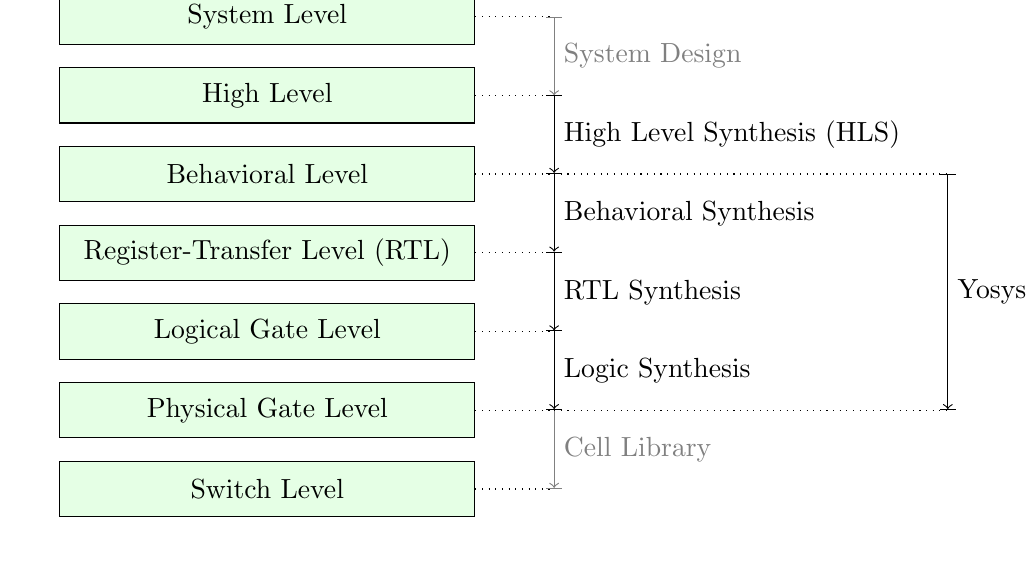
\begin{tikzpicture}
			\tikzstyle{lvl} = [draw, fill=green!10, rectangle, minimum height=2em, minimum width=15em]
			\node[lvl] (sys) {System Level};
			\node[lvl] (hl) [below of=sys] {High Level};
			\node[lvl] (beh) [below of=hl] {Behavioral Level};
			\node[lvl] (rtl) [below of=beh] {Register-Transfer Level (RTL)};
			\node[lvl] (lg) [below of=rtl] {Logical Gate Level};
			\node[lvl] (pg) [below of=lg] {Physical Gate Level};
			\node[lvl] (sw) [below of=pg] {Switch Level};

			\draw[dotted] (sys.east)  -- ++(1,0) coordinate (sysx);
			\draw[dotted] (hl.east)  -- ++(1,0) coordinate (hlx);
			\draw[dotted] (beh.east) -- ++(1,0) coordinate (behx);
			\draw[dotted] (rtl.east) -- ++(1,0) coordinate (rtlx);
			\draw[dotted] (lg.east)  -- ++(1,0) coordinate (lgx);
			\draw[dotted] (pg.east)  -- ++(1,0) coordinate (pgx);
			\draw[dotted] (sw.east)  -- ++(1,0) coordinate (swx);

			\draw[gray,|->] (sysx) -- node[right] {System Design} (hlx);
			\draw[|->|] (hlx) -- node[right] {High Level Synthesis (HLS)} (behx);
			\draw[->|] (behx) -- node[right] {Behavioral Synthesis} (rtlx);
			\draw[->|] (rtlx) -- node[right] {RTL Synthesis} (lgx);
			\draw[->|] (lgx) -- node[right] {Logic Synthesis} (pgx);
			\draw[gray,->|] (pgx) -- node[right] {Cell Library} (swx);

			\draw[dotted] (behx) -- ++(5,0) coordinate (a);
			\draw[dotted] (pgx) -- ++(5,0) coordinate (b);
			\draw[|->|] (a) -- node[right] {Yosys} (b);
	\end{tikzpicture}
	\caption{Different levels of abstraction and synthesis.}
	\label{fig:Basics_abstractions}
\end{figure}

Regardless of the way a lower level representation of a circuit is
obtained (synthesis or manual design), the lower level representation is usually
verified by comparing simulation results of the lower level and the higher level
representation \footnote{In recent years formal equivalence
checking also became an important verification method for validating RTL and
lower abstraction representation of the design.}.
Therefore even if no synthesis is used, there must still be a simulatable
representation of the circuit in all levels to allow for verification of the
design.

Note: The exact meaning of terminology such as ``High-Level'' is of course not
fixed over time. For example the HDL ``ABEL'' was first introduced in 1985 as ``A High-Level
Design Language for Programmable Logic Devices'' \cite{ABEL}, but would not
be considered a ``High-Level Language'' today.

\subsection{System Level}

The System Level abstraction of a system only looks at its biggest building
blocks like CPUs and computing cores. At this level the circuit is usually described
using traditional programming languages like C/C++ or Matlab. Sometimes special
software libraries are used that are aimed at simulation circuits on the system
level, such as SystemC.

Usually no synthesis tools are used to automatically transform a system level
representation of a circuit to a lower-level representation. But system level
design tools exist that can be used to connect system level building blocks.

The IEEE 1685-2009 standard defines the IP-XACT file format that can be used to
represent designs on the system level and building blocks that can be used in
such system level designs. \cite{IP-XACT}

\subsection{High Level}

The high-level abstraction of a system (sometimes referred to as {\it
algorithmic} level) is also often represented using traditional programming
languages, but with a reduced feature set. For example when representing a
design at the high level abstraction in C, pointers can only be used to mimic
concepts that can be found in hardware, such as memory interfaces. Full
featured dynamic memory management is not allowed as it has no corresponding
concept in digital circuits.

Tools exist to synthesize high level code (usually in the form of C/C++/SystemC
code with additional metadata) to behavioural HDL code (usually in the form of
Verilog or VHDL code). Aside from the many commercial tools for high level synthesis
there are also a number of FOSS tools for high level synthesis
\citeweblink{C_to_Verilog} \citeweblink{LegUp}.

\subsection{Behavioural Level}

At the behavioural abstraction level a language aimed at hardware description such
as Verilog or VHDL is used to describe the circuit, but so-called {\it behavioural
modelling} is used in at least part of the circuit description. In behavioural
modelling there must be a language feature that allows for imperative programming to be used to
describe data paths and registers. This is the {\tt always}-block in Verilog and
the {\tt process}-block in VHDL.

In behavioural modelling, code fragments are provided together with a {\it
sensitivity list}; a list of signals and conditions. In simulation, the code
fragment is executed whenever a signal in the sensitivity list changes its
value or a condition in the sensitivity list is triggered. A synthesis tool
must be able to transfer this representation into an appropriate datapath followed
by the appropriate types of register.

For example consider the following Verilog code fragment:

\begin{lstlisting}[numbers=left,frame=single,language=Verilog]
always @(posedge clk)
	y <= a + b;
\end{lstlisting}

In simulation the statement \lstinline[language=Verilog]{y <= a + b} is executed whenever
a positive edge on the signal \lstinline[language=Verilog]{clk} is detected. The synthesis
result however will contain an adder that calculates the sum \lstinline[language=Verilog]{a + b}
all the time, followed by a d-type flip-flop with the adder output on its D-input and the
signal \lstinline[language=Verilog]{y} on its Q-output.

Usually the imperative code fragments used in behavioural modelling can contain
statements for conditional execution (\lstinline[language=Verilog]{if}- and
\lstinline[language=Verilog]{case}-statements in Verilog) as well as loops,
as long as those loops can be completely unrolled.

Interestingly there seems to be no other FOSS Tool that is capable of
performing Verilog or VHDL behavioural syntheses besides Yosys (see
App.~\ref{chapter:sota}).

\subsection{Register-Transfer Level (RTL)}

On the Register-Transfer Level the design is represented by combinatorial data
paths and registers (usually d-type flip flops). The following Verilog code fragment
is equivalent to the previous Verilog example, but is in RTL representation:

\begin{lstlisting}[numbers=left,frame=single,language=Verilog]
assign tmp = a + b;       // combinatorial data path

always @(posedge clk)     // register
	y <= tmp;
\end{lstlisting}

A design in RTL representation is usually stored using HDLs like Verilog and VHDL. But only
a very limited subset of features is used, namely minimalistic {\tt always}-blocks (Verilog)
or {\tt process}-blocks (VHDL) that model the register type used and unconditional assignments
for the datapath logic. The use of HDLs on this level simplifies simulation as no additional
tools are required to simulate a design in RTL representation.

Many optimizations and analyses can be performed best at the RTL level. Examples include FSM
detection and optimization, identification of memories or other larger building blocks
and identification of shareable resources.

Note that RTL is the first abstraction level in which the circuit is represented as a
graph of circuit elements (registers and combinatorial cells) and signals. Such a graph,
when encoded as list of cells and connections, is called a netlist.

RTL synthesis is easy as each circuit node element in the netlist can simply be replaced
with an equivalent gate-level circuit. However, usually the term {\it RTL synthesis} does
not only refer to synthesizing an RTL netlist to a gate level netlist but also to performing
a number of highly sophisticated optimizations within the RTL representation, such as
the examples listed above.

A number of FOSS tools exist that can perform isolated tasks within the domain of RTL
synthesis steps. But there seems to be no FOSS tool that covers a wide range of RTL
synthesis operations.

\subsection{Logical Gate Level}

At the logical gate level the design is represented by a netlist that uses only
cells from a small number of single-bit cells, such as basic logic gates (AND,
OR, NOT, XOR, etc.) and registers (usually D-Type Flip-flops).

A number of netlist formats exists that can be used on this level, e.g.~the Electronic Design
Interchange Format (EDIF), but for ease of simulation often a HDL netlist is used. The latter
is a HDL file (Verilog or VHDL) that only uses the most basic language constructs for instantiation
and connecting of cells.

There are two challenges in logic synthesis: First finding opportunities for optimizations
within the gate level netlist and second the optimal (or at least good) mapping of the logic
gate netlist to an equivalent netlist of physically available gate types.

The simplest approach to logic synthesis is {\it two-level logic synthesis}, where a logic function
is converted into a sum-of-products representation, e.g.~using a Karnaugh map.
This is a simple approach, but has exponential worst-case effort and cannot make efficient use of
physical gates other than AND/NAND-, OR/NOR- and NOT-Gates.

Therefore modern logic synthesis tools utilize much more complicated {\it multi-level logic
synthesis} algorithms \cite{MultiLevelLogicSynth}. Most of these algorithms convert the
logic function to a Binary-Decision-Diagram (BDD) or And-Inverter-Graph (AIG) and work from that
representation. The former has the advantage that it has a unique normalized form. The latter has
much better worst case performance and is therefore better suited for the synthesis of large
logic functions.

Good FOSS tools exists for multi-level logic synthesis \citeweblink{ABC}
\citeweblink{AIGER} \citeweblink{MVSIS}.

Yosys contains basic logic synthesis functionality but can also use ABC
\citeweblink{ABC} for the logic synthesis step. Using ABC is recommended.

\subsection{Physical Gate Level}

On the physical gate level only gates are used that are physically available on
the target architecture. In some cases this may only be NAND, NOR and NOT gates as well as
D-Type registers. In other cases this might include cells that are more complex than the cells
used at the logical gate level (e.g.~complete half-adders). In the case of an FPGA-based
design the physical gate level representation is a netlist of LUTs with optional output
registers, as these are the basic building blocks of FPGA logic cells.

For the synthesis tool chain this abstraction is usually the lowest level. In
case of an ASIC-based design the cell library might contain further information on
how the physical cells map to individual switches (transistors).

\subsection{Switch Level}

A switch level representation of a circuit is a netlist utilizing single transistors as cells.
Switch level modelling is possible in Verilog and VHDL, but is seldom used in modern designs,
as in modern digital ASIC or FPGA flows the physical gates are considered the atomic build blocks
of the logic circuit.

\subsection{Yosys}

Yosys is a Verilog HDL synthesis tool. This means that it takes a behavioural
design description as input and generates an RTL, logical gate or physical gate
level description of the design as output.  Yosys' main strengths are behavioural
and RTL synthesis. A wide range of commands (synthesis passes) exist
within Yosys that can be used to perform a wide range of synthesis tasks within
the domain of behavioural, rtl and logic synthesis. Yosys is designed to be
extensible and therefore is a good basis for implementing custom synthesis
tools for specialised tasks.

\section{Features of Synthesizable Verilog}

The subset of Verilog \cite{Verilog2005} that is synthesizable is specified in
a separate IEEE standards document, the IEEE standard 1364.1-2002 \cite{VerilogSynth}.
This standard also describes how certain language constructs are to be interpreted in
the scope of synthesis.

This section provides a quick overview of the most important features of
synthesizable Verilog, structured in order of increasing complexity.

\subsection{Structural Verilog}

{\it Structural Verilog} (also known as {\it Verilog Netlists}) is a Netlist in
Verilog syntax. Only the following language constructs are used in this case:

\begin{itemize}
\item Constant values
\item Wire and port declarations
\item Static assignments of signals to other signals
\item Cell instantiations
\end{itemize}

Many tools (especially at the back end of the synthesis chain) only support
structural Verilog as input. ABC is an example of such a tool. Unfortunately
there is no standard specifying what {\it Structural Verilog} actually is,
leading to some confusion about what syntax constructs are supported in
structural Verilog when it comes to features such as attributes or multi-bit
signals.

\subsection{Expressions in Verilog}

In all situations where Verilog accepts a constant value or signal name,
expressions using arithmetic operations such as
\lstinline[language=Verilog]{+}, \lstinline[language=Verilog]{-} and \lstinline[language=Verilog]{*},
boolean operations such as
\lstinline[language=Verilog]{&} (AND), \lstinline[language=Verilog]{|} (OR) and \lstinline[language=Verilog]{^} (XOR)
and many others (comparison operations, unary operator, etc.) can also be used.

During synthesis these operators are replaced by cells that implement the respective function.

Many FOSS tools that claim to be able to process Verilog in fact only support
basic structural Verilog and simple expressions. Yosys can be used to convert
full featured synthesizable Verilog to this simpler subset, thus enabling such
applications to be used with a richer set of Verilog features.

\subsection{Behavioural Modelling}

Code that utilizes the Verilog {\tt always} statement is using {\it Behavioural
Modelling}. In behavioural modelling, a circuit is described by means of imperative
program code that is executed on certain events, namely any change, a rising
edge, or a falling edge of a signal. This is a very flexible construct during
simulation but is only synthesizable when one of the following is modelled:

\begin{itemize}
\item {\bf Asynchronous or latched logic} \\
In this case the sensitivity list must contain all expressions that are used within
the {\tt always} block. The syntax \lstinline[language=Verilog]{@*} can be used
for these cases. Examples of this kind include:

\begin{lstlisting}[numbers=left,frame=single,language=Verilog]
// asynchronous
always @* begin
	if (add_mode)
		y <= a + b;
	else
		y <= a - b;
end

// latched
always @* begin
	if (!hold)
		y <= a + b;
end
\end{lstlisting}

Note that latched logic is often considered bad style and in many cases just
the result of sloppy HDL design. Therefore many synthesis tools generate warnings
whenever latched logic is generated.

\item {\bf Synchronous logic (with optional synchronous reset)} \\
This is logic with d-type flip-flops on the output. In this case the sensitivity
list must only contain the respective clock edge. Example:
\begin{lstlisting}[numbers=left,frame=single,language=Verilog]
// counter with synchronous reset
always @(posedge clk) begin
	if (reset)
		y <= 0;
	else
		y <= y + 1;
end
\end{lstlisting}

\item {\bf Synchronous logic with asynchronous reset} \\
This is logic with d-type flip-flops with asynchronous resets on the output. In
this case the sensitivity list must only contain the respective clock and reset edges.
The values assigned in the reset branch must be constant. Example:
\begin{lstlisting}[numbers=left,frame=single,language=Verilog]
// counter with asynchronous reset
always @(posedge clk, posedge reset) begin
	if (reset)
		y <= 0;
	else
		y <= y + 1;
end
\end{lstlisting}
\end{itemize}

Many synthesis tools support a wider subset of flip-flops that can be modelled
using {\tt always}-statements (including Yosys). But only the ones listed above
are covered by the Verilog synthesis standard and when writing new designs one
should limit herself or himself to these cases.

In behavioural modelling, blocking assignments (=) and non-blocking assignments
(<=) can be used. The concept of blocking vs.~non-blocking assignment is one
of the most misunderstood constructs in Verilog \cite{Cummings00}.

The blocking assignment behaves exactly like an assignment in any imperative
programming language, while with the non-blocking assignment the right hand side
of the assignment is evaluated immediately but the actual update of the left
hand side register is delayed until the end of the time-step. For example the Verilog
code \lstinline[language=Verilog]{a <= b; b <= a;} exchanges the values of
the two registers. See Sec.~\ref{sec:blocking_nonblocking} for a more
detailed description of this behaviour.

\subsection{Functions and Tasks}

Verilog supports {\it Functions} and {\it Tasks} to bundle statements that are
used in multiple places (similar to {\it Procedures} in imperative programming).
Both constructs can be implemented easily by substituting the function/task-call
with the body of the function or task.

\subsection{Conditionals, Loops and Generate-Statements}

Verilog supports \lstinline[language=Verilog]{if-else}-statements and
\lstinline[language=Verilog]{for}-loops inside \lstinline[language=Verilog]{always}-statements.

It also supports both features in \lstinline[language=Verilog]{generate}-statements
on the module level. This can be used to selectively enable or disable parts of the
module based on the module parameters (\lstinline[language=Verilog]{if-else})
or to generate a set of similar subcircuits (\lstinline[language=Verilog]{for}).

While the \lstinline[language=Verilog]{if-else}-statement
inside an always-block is part of behavioural modelling, the three other cases
are (at least for a synthesis tool) part of a built-in macro processor. Therefore it must
be possible for the synthesis tool to completely unroll all loops and evaluate the
condition in all \lstinline[language=Verilog]{if-else}-statement in
\lstinline[language=Verilog]{generate}-statements using const-folding.

Examples for this can be found in Fig.~\ref{fig:StateOfTheArt_for} and
Fig.~\ref{fig:StateOfTheArt_gen} in App.~\ref{chapter:sota}.

\subsection{Arrays and Memories}

Verilog supports arrays. This is in general a synthesizable language feature.
In most cases arrays can be synthesized by generating addressable memories.
However, when complex or asynchronous access patterns are used, it is not
possible to model an array as memory. In these cases the array must
be modelled using individual signals for each word and all accesses to the array
must be implemented using large multiplexers.

In some cases it would be possible to model an array using memories, but it
is not desired. Consider the following delay circuit:
\begin{lstlisting}[numbers=left,frame=single,language=Verilog]
module (clk, in_data, out_data);

parameter BITS = 8;
parameter STAGES = 4;

input clk;
input [BITS-1:0] in_data;
output [BITS-1:0] out_data;
reg [BITS-1:0] ffs [STAGES-1:0];

integer i;
always @(posedge clk) begin
	ffs[0] <= in_data;
	for (i = 1; i < STAGES; i = i+1)
		ffs[i] <= ffs[i-1];
end

assign out_data = ffs[STAGES-1];

endmodule
\end{lstlisting}

This could be implemented using an addressable memory with {\tt STAGES} input
and output ports. A better implementation would be to use a simple chain of flip-flops
(a so-called shift register).
This better implementation can either be obtained by first creating a memory-based
implementation and then optimizing it based on the static address signals for all ports
or directly identifying such situations in the language front end and converting
all memory accesses to direct accesses to the correct signals.

\section{Challenges in Digital Circuit Synthesis}

This section summarizes the most important challenges in digital circuit
synthesis. Tools can be characterized by how well they address these topics.

\subsection{Standards Compliance}

The most important challenge is compliance with the HDL standards in question (in case
of Verilog the IEEE Standards 1364.1-2002 and 1364-2005). This can be broken down in two
items:

\begin{itemize}
\item Completeness of implementation of the standard
\item Correctness of implementation of the standard
\end{itemize}

Completeness is mostly important to guarantee compatibility
with existing HDL code. Once a design has been verified and tested, HDL designers
are very reluctant regarding changes to the design, even if it is only about
a few minor changes to work around a missing feature in a new synthesis tool.

Correctness is crucial. In some areas this is obvious (such as
correct synthesis of basic behavioural models). But it is also crucial for the
areas that concern minor details of the standard, such as the exact rules
for handling signed expressions, even when the HDL code does not target
different synthesis tools. This is because (unlike software source code that
is only processed by compilers), in most design flows HDL code is not only
processed by the synthesis tool but also by one or more simulators and sometimes
even a formal verification tool. It is key for this verification process
that all these tools use the same interpretation for the HDL code.

\subsection{Optimizations}

Generally it is hard to give a one-dimensional description of how well a synthesis tool
optimizes the design. First of all because not all optimizations are applicable to all
designs and all synthesis tasks. Some optimizations work (best) on a coarse-grained level
(with complex cells such as adders or multipliers) and others work (best) on a fine-grained
level (single bit gates). Some optimizations target area and others target speed.
Some work well on large designs while others don't scale well and can only be applied
to small designs.

A good tool is capable of applying a wide range of optimizations at different
levels of abstraction and gives the designer control over which optimizations
are performed (or skipped) and what the optimization goals are.

\subsection{Technology Mapping}

Technology mapping is the process of converting the design into a netlist of
cells that are available in the target architecture. In an ASIC flow this might
be the process-specific cell library provided by the fab. In an FPGA flow this
might be LUT cells as well as special function units such as dedicated multipliers.
In a coarse-grain flow this might even be more complex special function units.

An open and vendor independent tool is especially of interest if it supports
a wide range of different types of target architectures.

\section{Script-Based Synthesis Flows}

A digital design is usually started by implementing a high-level or
system-level simulation of the desired function. This description is then
manually transformed (or re-implemented) into a synthesizable lower-level
description (usually at the behavioural level) and the equivalence of the
two representations is verified by simulating both and comparing the simulation
results.

Then the synthesizable description is transformed to lower-level
representations using a series of tools and the results are again verified
using simulation. This process is illustrated in Fig.~\ref{fig:Basics_flow}.

\begin{figure}[t!]
	\hfil
	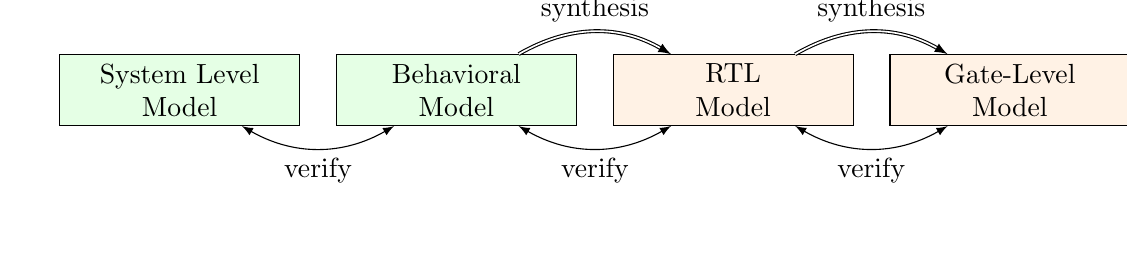
\begin{tikzpicture}
			\tikzstyle{manual} = [draw, fill=green!10, rectangle, minimum height=2em, minimum width=8em, node distance=10em]
			\tikzstyle{auto} = [draw, fill=orange!10, rectangle, minimum height=2em, minimum width=8em, node distance=10em]

			\node[manual] (sys) {\begin{minipage}{8em}
				\center
				System Level \\
				Model
			\end{minipage}};
			\node[manual] (beh) [right of=sys] {\begin{minipage}{8em}
				\center
				Behavioral \\
				Model
			\end{minipage}};
			\node[auto] (rtl) [right of=beh] {\begin{minipage}{8em}
				\center
				RTL \\
				Model
			\end{minipage}};
			\node[auto] (gates) [right of=rtl] {\begin{minipage}{8em}
				\center
				Gate-Level \\
				Model
			\end{minipage}};

			\draw[-latex] (beh) edge[double, bend left] node[above] {synthesis} (rtl);
			\draw[-latex] (rtl) edge[double, bend left] node[above] {synthesis} (gates);

			\draw[latex-latex] (sys) edge[bend right] node[below] {verify} (beh);
			\draw[latex-latex] (beh) edge[bend right] node[below] {verify} (rtl);
			\draw[latex-latex] (rtl) edge[bend right] node[below] {verify} (gates);
	\end{tikzpicture}
	\caption{Typical design flow. Green boxes represent manually created models. Orange boxes represent
	models generated by synthesis tools.}
	\label{fig:Basics_flow}
\end{figure}

In this example the System Level Model and the Behavioural Model are both
manually written design files. After the equivalence of system level model
and behavioural model has been verified, the lower level representations of the
design can be generated using synthesis tools. Finally the RTL Model and
the Gate-Level Model are verified and the design process is finished.

However, in any real-world design effort there will be multiple iterations for
this design process. The reason for this can be the late change of a design
requirement or the fact that the analysis of a low-abstraction model (e.g.~gate-level
timing analysis) revealed that a design change is required in order to meet
the design requirements (e.g.~maximum possible clock speed).

Whenever the behavioural model or the system level model is
changed their equivalence must be re-verified by re-running the simulations
and comparing the results. Whenever the behavioural model is changed the
synthesis must be re-run and the synthesis results must be re-verified.

In order to guarantee reproducibility it is important to be able to re-run all
automatic steps in a design project with a fixed set of settings easily.
Because of this, usually all programs used in a synthesis flow can be
controlled using scripts. This means that all functions are available via
text commands. When such a tool provides a GUI, this is complementary to,
and not instead of, a command line interface.

Usually a synthesis flow in an UNIX/Linux environment would be controlled by a
shell script that calls all required tools (synthesis and simulation/verification
in this example) in the correct order. Each of these tools would be called with
a script file containing commands for the respective tool. All settings required
for the tool would be provided by these script files so that no manual interaction
would be necessary. These script files are considered design sources and should
be kept under version control just like the source code of the system level and the
behavioural model.

\section{Methods from Compiler Design}

Some parts of synthesis tools involve problem domains that are traditionally known from
compiler design. This section addresses some of these domains.

\subsection{Lexing and Parsing}

The best known concepts from compiler design are probably {\it lexing} and {\it parsing}.
These are two methods that together can be used to process complex computer languages
easily. \cite{Dragonbook}

A {\it lexer} consumes single characters from the input and generates a stream of {\it lexical
tokens} that consist of a {\it type} and a {\it value}. For example the Verilog input
``\lstinline[language=Verilog]{assign foo = bar + 42;}'' might be translated by the lexer
to the list of lexical tokens given in Tab.~\ref{tab:Basics_tokens}.

\begin{table}[t]
\hfil
\begin{tabular}{ll}
Token-Type & Token-Value \\
\hline
\tt TOK\_ASSIGN & - \\
\tt TOK\_IDENTIFIER & ``{\tt foo}'' \\
\tt TOK\_EQ & - \\
\tt TOK\_IDENTIFIER & ``{\tt bar}'' \\
\tt TOK\_PLUS & - \\
\tt TOK\_NUMBER & 42 \\
\tt TOK\_SEMICOLON & - \\
\end{tabular}
\caption{Exemplary token list for the statement ``\lstinline[language=Verilog]{assign foo = bar + 42;}''.}
\label{tab:Basics_tokens}
\end{table}

The lexer is usually generated by a lexer generator (e.g.~{\tt flex} \citeweblink{flex}) from a
description file that is using regular expressions to specify the text pattern that should match
the individual tokens.

The lexer is also responsible for skipping ignored characters (such as whitespace outside string
constants and comments in the case of Verilog) and converting the original text snippet to a token
value.

Note that individual keywords use different token types (instead of a keyword type with different
token values). This is because the parser usually can only use the Token-Type to make a decision on
the grammatical role of a token.

The parser then transforms the list of tokens into a parse tree that closely resembles the productions
from the computer languages grammar. As the lexer, the parser is also typically generated by a code
generator (e.g.~{\tt bison} \citeweblink{bison}) from a grammar description in Backus-Naur Form (BNF).

Let's consider the following BNF (in Bison syntax):

\begin{lstlisting}[numbers=left,frame=single]
assign_stmt: TOK_ASSIGN TOK_IDENTIFIER TOK_EQ expr TOK_SEMICOLON;
expr: TOK_IDENTIFIER | TOK_NUMBER | expr TOK_PLUS expr;
\end{lstlisting}

\begin{figure}[b!]
	\hfil
	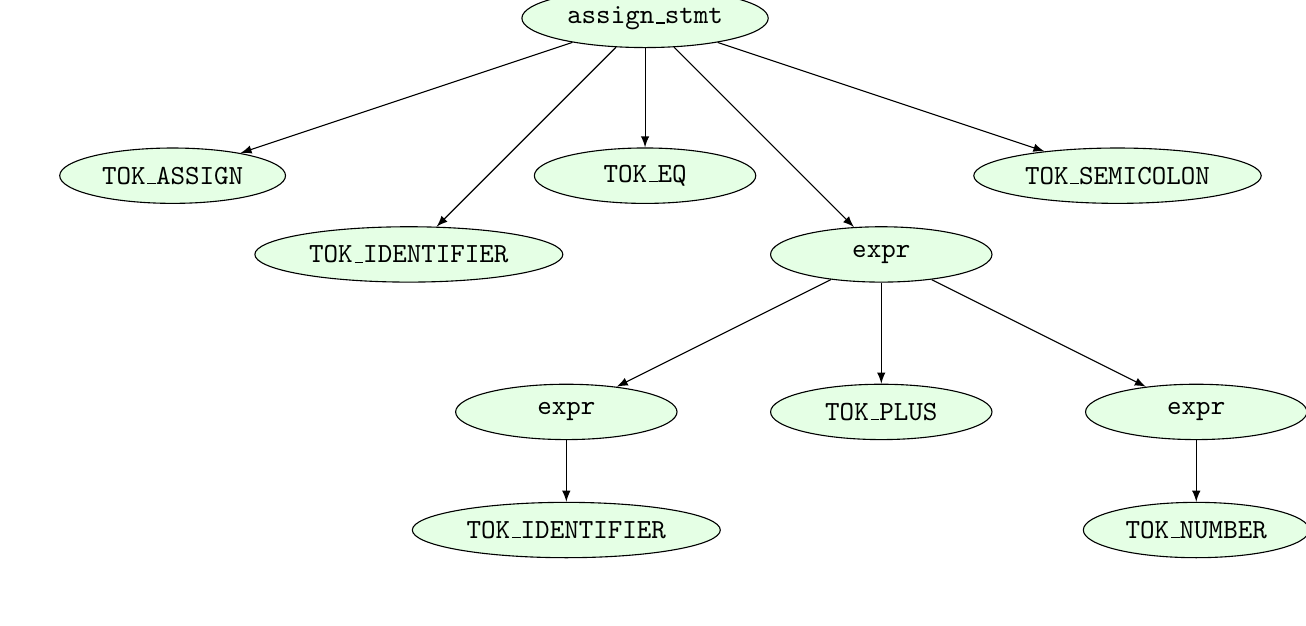
\begin{tikzpicture}
			\tikzstyle{node} = [draw, fill=green!10, ellipse, minimum height=2em, minimum width=8em, node distance=10em]

			\draw (+0,+1) node[node] (n1) {\tt assign\_stmt};

			\draw (-6,-1) node[node] (n11) {\tt TOK\_ASSIGN};
			\draw (-3,-2) node[node] (n12) {\tt TOK\_IDENTIFIER};
			\draw (+0,-1) node[node] (n13) {\tt TOK\_EQ};
			\draw (+3,-2) node[node] (n14) {\tt expr};
			\draw (+6,-1) node[node] (n15) {\tt TOK\_SEMICOLON};

			\draw (-1,-4) node[node] (n141) {\tt expr};
			\draw (+3,-4) node[node] (n142) {\tt TOK\_PLUS};
			\draw (+7,-4) node[node] (n143) {\tt expr};

			\draw (-1,-5.5) node[node] (n1411) {\tt TOK\_IDENTIFIER};
			\draw (+7,-5.5) node[node] (n1431) {\tt TOK\_NUMBER};

			\draw[-latex] (n1) -- (n11);
			\draw[-latex] (n1) -- (n12);
			\draw[-latex] (n1) -- (n13);
			\draw[-latex] (n1) -- (n14);
			\draw[-latex] (n1) -- (n15);

			\draw[-latex] (n14) -- (n141);
			\draw[-latex] (n14) -- (n142);
			\draw[-latex] (n14) -- (n143);

			\draw[-latex] (n141) -- (n1411);
			\draw[-latex] (n143) -- (n1431);
	\end{tikzpicture}
	\caption{Example parse tree for the Verilog expression ``\lstinline[language=Verilog]{assign foo = bar + 42;}''.}
	\label{fig:Basics_parsetree}
\end{figure}

The parser converts the token list to the parse tree in Fig.~\ref{fig:Basics_parsetree}. Note that the parse
tree never actually exists as a whole as data structure in memory. Instead the parser calls user-specified
code snippets (so-called {\it reduce-functions}) for all inner nodes of the parse tree in depth-first order.

In some very simple applications (e.g.~code generation for stack machines) it is possible to perform the
task at hand directly in the reduce functions. But usually the reduce functions are only used to build an in-memory
data structure with the relevant information from the parse tree. This data structure is called an {\it abstract
syntax tree} (AST).

The exact format for the abstract syntax tree is application specific (while the format of the parse tree and token
list are mostly dictated by the grammar of the language at hand). Figure~\ref{fig:Basics_ast} illustrates what an
AST for the parse tree in Fig.~\ref{fig:Basics_parsetree} could look like.

Usually the AST is then converted into yet another representation that is more suitable for further processing.
In compilers this is often an assembler-like three-address-code intermediate representation. \cite{Dragonbook}

\begin{figure}[t]
	\hfil
	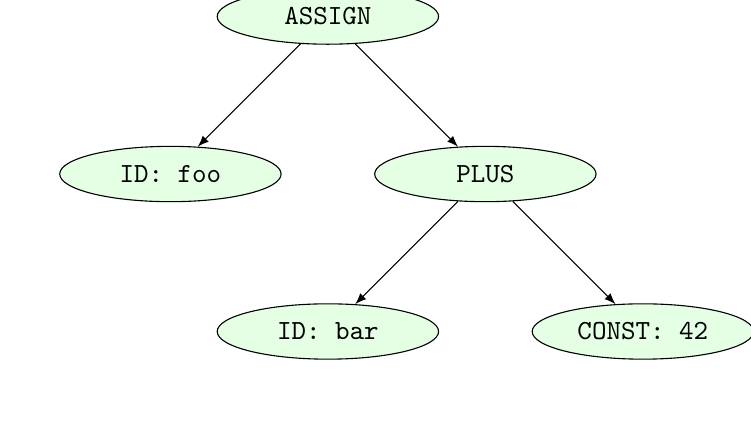
\begin{tikzpicture}
			\tikzstyle{node} = [draw, fill=green!10, ellipse, minimum height=2em, minimum width=8em, node distance=10em]

			\draw (+0,+0) node[node] (n1) {\tt ASSIGN};

			\draw (-2,-2) node[node] (n11) {\tt ID: foo};
			\draw (+2,-2) node[node] (n12) {\tt PLUS};

			\draw (+0,-4) node[node] (n121) {\tt ID: bar};
			\draw (+4,-4) node[node] (n122) {\tt CONST: 42};

			\draw[-latex] (n1) -- (n11);
			\draw[-latex] (n1) -- (n12);

			\draw[-latex] (n12) -- (n121);
			\draw[-latex] (n12) -- (n122);
	\end{tikzpicture}
	\caption{Example abstract syntax tree for the Verilog expression ``\lstinline[language=Verilog]{assign foo = bar + 42;}''.}
	\label{fig:Basics_ast}
\end{figure}

\subsection{Multi-Pass Compilation}

Complex problems are often best solved when split up into smaller problems. This is certainly true
for compilers as well as for synthesis tools. The components responsible for solving the smaller problems can
be connected in two different ways: through {\it Single-Pass Pipelining} and by using {\it Multiple Passes}.

Traditionally a parser and lexer are connected using the pipelined approach: The lexer provides a function that
is called by the parser. This function reads data from the input until a complete lexical token has been read. Then
this token is returned to the parser. So the lexer does not first generate a complete list of lexical tokens
and then pass it to the parser. Instead they run concurrently and the parser can consume tokens as
the lexer produces them.

The single-pass pipelining approach has the advantage of lower memory footprint (at no time must the complete design
be kept in memory) but has the disadvantage of tighter coupling between the interacting components.

Therefore single-pass pipelining should only be used when the lower memory footprint is required or the
components are also conceptually tightly coupled. The latter certainly is the case for a parser and its lexer.
But when data is passed between two conceptually loosely coupled components it is often
beneficial to use a multi-pass approach.

In the multi-pass approach the first component processes all the data and the result is stored in a in-memory
data structure. Then the second component is called with this data. This reduces complexity, as only one
component is running at a time. It also improves flexibility as components can be exchanged easier.

Most modern compilers are multi-pass compilers.

\iffalse
\subsection{Static Single Assignment Form}

In imperative programming (and behavioural HDL design) it is possible to assign the same variable multiple times.
This can either mean that the variable is independently used in two different contexts or that the final value
of the variable depends on a condition.

The following examples show C code in which one variable is used independently in two different contexts:

\begin{minipage}{7.7cm}
\begin{lstlisting}[numbers=left,frame=single,language=C++]
void demo1()
{
	int a = 1;
	printf("%d\n", a);

	a = 2;
	printf("%d\n", a);
}
\end{lstlisting}
\end{minipage}
\hfil
\begin{minipage}{7.7cm}
\begin{lstlisting}[frame=single,language=C++]
void demo1()
{
	int a = 1;
	printf("%d\n", a);

	int b = 2;
	printf("%d\n", b);
}
\end{lstlisting}
\end{minipage}

\begin{minipage}{7.7cm}
\begin{lstlisting}[numbers=left,frame=single,language=C++]
void demo2(bool foo)
{
	int a;
	if (foo) {
		a = 23;
		printf("%d\n", a);
	} else {
		a = 42;
		printf("%d\n", a);
	}
}
\end{lstlisting}
\end{minipage}
\hfil
\begin{minipage}{7.7cm}
\begin{lstlisting}[frame=single,language=C++]
void demo2(bool foo)
{
	int a, b;
	if (foo) {
		a = 23;
		printf("%d\n", a);
	} else {
		b = 42;
		printf("%d\n", b);
	}
}
\end{lstlisting}
\end{minipage}

In both examples the left version (only variable \lstinline[language=C++]{a}) and the right version (variables
\lstinline[language=Verilog]{a} and \lstinline[language=Verilog]{b}) are equivalent. Therefore it is
desired for further processing to bring the code in an equivalent form for both cases.

In the following example the variable is assigned twice but it cannot be easily replaced by two variables:

\begin{lstlisting}[frame=single,language=C++]
void demo3(bool foo)
{
	int a = 23
	if (foo)
		a = 42;
	printf("%d\n", a);
}
\end{lstlisting}

Static single assignment (SSA) form is a representation of imperative code that uses identical representations
for the left and right version of demos 1 and 2, but can still represent demo 3. In SSA form each assignment
assigns a new variable (usually written with an index). But it also introduces a special $\Phi$-function to
merge the different instances of a variable when needed. In C-pseudo-code the demo 3 would be written as follows
using SSA from:

\begin{lstlisting}[frame=single,language=C++]
void demo3(bool foo)
{
	int a_1, a_2, a_3;
	a_1 = 23
	if (foo)
		a_2 = 42;
	a_3 = phi(a_1, a_2);
	printf("%d\n", a_3);
}
\end{lstlisting}

The $\Phi$-function is usually interpreted as ``these variables must be stored
in the same memory location'' during code generation. Most modern compilers for imperative languages
such as C/C++ use SSA form for at least some of its passes as it is very easy to manipulate and analyse.
\fi



\chapter{Approach}
\label{chapter:approach}

Yosys is a tool for synthesising (behavioural) Verilog HDL code to target architecture netlists. Yosys aims at a wide
range of application domains and thus must be flexible and easy to adapt to new tasks. This chapter covers the general
approach followed in the effort to implement this tool.

\section{Data- and Control-Flow}

The data- and control-flow of a typical synthesis tool is very similar to the data- and control-flow of a typical
compiler: different subsystems are called in a predetermined order, each consuming the data generated by the
last subsystem and generating the data for the next subsystem (see Fig.~\ref{fig:approach_flow}).

\begin{figure}[b]
	\hfil
	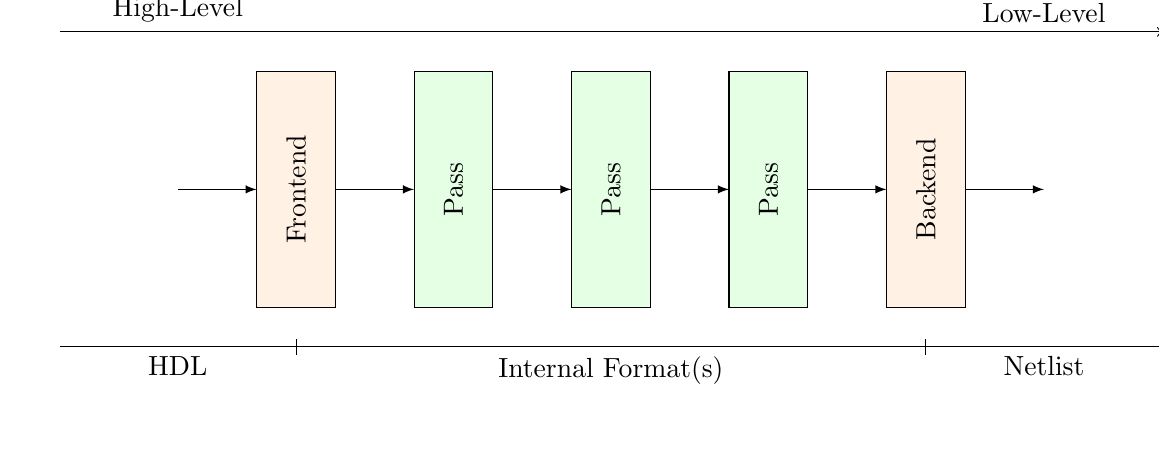
\begin{tikzpicture}
		\path (-1.5,3) coordinate (cursor);
		\draw[-latex] ($ (cursor) + (0,-1.5) $) -- ++(1,0);
		\draw[fill=orange!10] ($ (cursor) + (1,-3) $) rectangle node[rotate=90] {Frontend} ++(1,3) coordinate (cursor);
		\draw[-latex] ($ (cursor) + (0,-1.5) $) -- ++(1,0);
		\draw[fill=green!10] ($ (cursor) + (1,-3) $) rectangle node[rotate=90] {Pass} ++(1,3) coordinate (cursor);
		\draw[-latex] ($ (cursor) + (0,-1.5) $) -- ++(1,0);
		\draw[fill=green!10] ($ (cursor) + (1,-3) $) rectangle node[rotate=90] {Pass} ++(1,3) coordinate (cursor);
		\draw[-latex] ($ (cursor) + (0,-1.5) $) -- ++(1,0);
		\draw[fill=green!10] ($ (cursor) + (1,-3) $) rectangle node[rotate=90] {Pass} ++(1,3) coordinate (cursor);
		\draw[-latex] ($ (cursor) + (0,-1.5) $) -- ++(1,0);
		\draw[fill=orange!10] ($ (cursor) + (1,-3) $) rectangle node[rotate=90] {Backend} ++(1,3) coordinate (cursor);
		\draw[-latex] ($ (cursor) + (0,-1.5) $) -- ++(1,0);

		\path (-3,-0.5) coordinate (cursor);
		\draw (cursor) -- node[below] {HDL} ++(3,0) coordinate (cursor);
		\draw[|-|] (cursor) -- node[below] {Internal Format(s)} ++(8,0) coordinate (cursor);
		\draw (cursor) -- node[below] {Netlist} ++(3,0);

		\path (-3,3.5) coordinate (cursor);
		\draw[-] (cursor) -- node[above] {High-Level} ++(3,0) coordinate (cursor);
		\draw[-] (cursor) -- ++(8,0) coordinate (cursor);
		\draw[->] (cursor) -- node[above] {Low-Level} ++(3,0);

	\end{tikzpicture}
	\caption{General data- and control-flow of a synthesis tool}
	\label{fig:approach_flow}
\end{figure}

The first subsystem to be called is usually called a {\it frontend}. It does not process the data generated by
another subsystem but instead reads the user input---in the case of a HDL synthesis tool, the behavioural
HDL code.

The subsystems that consume data from previous subsystems and produce data for the next subsystems (usually in the
same or a similar format) are called {\it passes}.

The last subsystem that is executed transforms the data generated by the last pass into a suitable output
format and writes it to a disk file. This subsystem is usually called the {\it backend}.

In Yosys all frontends, passes and backends are directly available as commands in the synthesis script. Thus
the user can easily create a custom synthesis flow just by calling passes in the right order in a synthesis
script.

\section{Internal Formats in Yosys}

Yosys uses two different internal formats. The first is used to store an abstract syntax tree (AST) of a Verilog
input file. This format is simply called {\it AST} and is generated by the Verilog Frontend. This data structure
is consumed by a subsystem called {\it AST Frontend}\footnote{In Yosys the term {\it pass} is only used to
refer to commands that operate on the RTLIL data structure.}. This AST Frontend then generates a design in Yosys'
main internal format, the Register-Transfer-Level-Intermediate-Language (RTLIL) representation. It does that
by first performing a number of simplifications within the AST representation and then generating RTLIL from
the simplified AST data structure.

The RTLIL representation is used by all passes as input and outputs. This has the following advantages over
using different representational formats between different passes:

\begin{itemize}
\item The passes can be rearranged in a different order and passes can be removed or inserted.
\item Passes can simply pass-thru the parts of the design they don't change without the need
      to convert between formats. In fact Yosys passes output the same data structure they received
      as input and performs all changes in place.
\item All passes use the same interface, thus reducing the effort required to understand a pass
      when reading the Yosys source code, e.g.~when adding additional features.
\end{itemize}

The RTLIL representation is basically a netlist representation with the following additional features:

\begin{itemize}
\item An internal cell library with fixed-function cells to represent RTL datapath and register cells as well
as logical gate-level cells (single-bit gates and registers).
\item Support for multi-bit values that can use individual bits from wires as well as constant bits to
represent coarse-grain netlists.
\item Support for basic behavioural constructs (if-then-else structures and multi-case switches with
a sensitivity list for updating the outputs).
\item Support for multi-port memories.
\end{itemize}

The use of RTLIL also has the disadvantage of having a very powerful format
between all passes, even when doing gate-level synthesis where the more
advanced features are not needed. In order to reduce complexity for passes that
operate on a low-level representation, these passes check the features used in
the input RTLIL and fail to run when unsupported high-level constructs are
used. In such cases a pass that transforms the higher-level constructs to
lower-level constructs must be called from the synthesis script first.

\section{Typical Use Case}
\label{sec:typusecase}

The following example script may be used in a synthesis flow to convert the behavioural Verilog code
from the input file {\tt design.v} to a gate-level netlist {\tt synth.v} using the cell library
described by the Liberty file \citeweblink{LibertyFormat} {\tt cells.lib}:

\begin{lstlisting}[language=sh,numbers=left,frame=single]
# read input file to internal representation
read_verilog design.v

# convert high-level behavioral parts ("processes") to d-type flip-flops and muxes
proc

# perform some simple optimizations
opt

# convert high-level memory constructs to d-type flip-flops and multiplexers
memory

# perform some simple optimizations
opt

# convert design to (logical) gate-level netlists
techmap

# perform some simple optimizations
opt

# map internal register types to the ones from the cell library
dfflibmap -liberty cells.lib

# use ABC to map remaining logic to cells from the cell library
abc -liberty cells.lib

# cleanup
opt

# write results to output file
write_verilog synth.v
\end{lstlisting}

A detailed description of the commands available in Yosys can be found in App.~\ref{commandref}.



\chapter{Implementation Overview}
\label{chapter:overview}

Yosys is an extensible open source hardware synthesis tool. It is aimed at
designers who are looking for an easily accessible, universal, and
vendor-independent synthesis tool, as well as scientists who do research in
electronic design automation (EDA) and are looking for an open synthesis
framework that can be used to test algorithms on complex real-world designs.

Yosys can synthesize a large subset of Verilog 2005 and has been tested with a
wide range of real-world designs, including the OpenRISC 1200 CPU
\citeweblink{OR1200}, the openMSP430 CPU \citeweblink{openMSP430}, the
OpenCores I$^2$C master \citeweblink{i2cmaster} and the k68 CPU \citeweblink{k68}.

As of this writing a Yosys VHDL frontend is in development.

Yosys is written in C++ (using some features from the new C++11 standard). This
chapter describes some of the fundamental Yosys data structures. For the sake
of simplicity the C++ type names used in the Yosys implementation are used in
this chapter, even though the chapter only explains the conceptual idea behind
it and can be used as reference to implement a similar system in any language.

\section{Simplified Data Flow}

Figure~\ref{fig:Overview_flow} shows the simplified data flow within Yosys.
Rectangles in the figure represent program modules and ellipses internal
data structures that are used to exchange design data between the program
modules.

Design data is read in using one of the frontend modules. The high-level HDL
frontends for Verilog and VHDL code generate an abstract syntax tree (AST) that
is then passed to the AST frontend. Note that both HDL frontends use the same
AST representation that is powerful enough to cover the Verilog HDL and VHDL
language.

The AST Frontend then compiles the AST to Yosys's main internal data format,
the RTL Intermediate Language (RTLIL). A more detailed description of this format
is given in the next section.

There is also a text representation of the RTLIL data structure that can be
parsed using the ILANG Frontend.

The design data may then be transformed using a series of passes that all
operate on the RTLIL representation of the design.

Finally the design in RTLIL representation is converted back to text by one
of the backends, namely the Verilog Backend for generating Verilog netlists
and the ILANG Backend for writing the RTLIL data in the same format that is
understood by the ILANG Frontend.

With the exception of the AST Frontend, which is called by the high-level HDL
frontends and can't be called directly by the user, all program modules are
called by the user (usually using a synthesis script that contains text
commands for Yosys).

By combining passes in different ways and/or adding additional passes to Yosys
it is possible to adapt Yosys to a wide range of applications. For this to be
possible it is key that (1) all passes operate on the same data structure
(RTLIL) and (2) that this data structure is powerful enough to represent the design
in different stages of the synthesis.

\begin{figure}[t]
	\hfil
	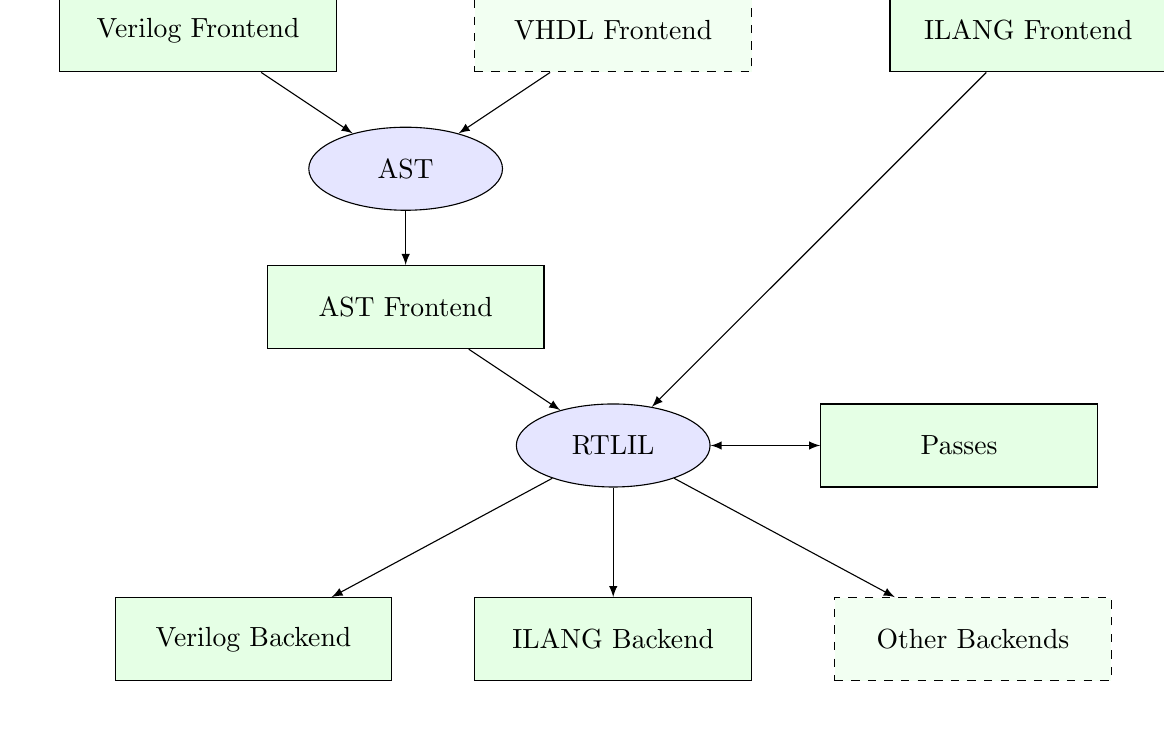
\begin{tikzpicture}
		\tikzstyle{process} = [draw, fill=green!10, rectangle, minimum height=3em, minimum width=10em, node distance=15em]
		\tikzstyle{data} = [draw, fill=blue!10, ellipse, minimum height=3em, minimum width=7em, node distance=15em]
		\node[process] (vlog) {Verilog Frontend};
		\node[process, dashed, fill=green!5] (vhdl) [right of=vlog] {VHDL Frontend};
		\node[process] (ilang) [right of=vhdl] {ILANG Frontend};
		\node[data] (ast) [below of=vlog, node distance=5em, xshift=7.5em] {AST};
		\node[process] (astfe) [below of=ast, node distance=5em] {AST Frontend};
		\node[data] (rtlil) [below of=astfe, node distance=5em, xshift=7.5em] {RTLIL};
		\node[process] (pass) [right of=rtlil, node distance=5em, xshift=7.5em] {Passes};
		\node[process] (vlbe) [below of=rtlil, node distance=7em, xshift=-13em] {Verilog Backend};
		\node[process] (ilangbe) [below of=rtlil, node distance=7em, xshift=0em] {ILANG Backend};
		\node[process, dashed, fill=green!5] (otherbe) [below of=rtlil, node distance=7em, xshift=+13em] {Other Backends};

		\draw[-latex] (vlog) -- (ast);
		\draw[-latex] (vhdl) -- (ast);
		\draw[-latex] (ast) -- (astfe);
		\draw[-latex] (astfe) -- (rtlil);
		\draw[-latex] (ilang) -- (rtlil);
		\draw[latex-latex] (rtlil) -- (pass);
		\draw[-latex] (rtlil) -- (vlbe);
		\draw[-latex] (rtlil) -- (ilangbe);
		\draw[-latex] (rtlil) -- (otherbe);
	\end{tikzpicture}
	\caption{Yosys simplified data flow (ellipses: data structures, rectangles: program modules)}
	\label{fig:Overview_flow}
\end{figure}

\section{The RTL Intermediate Language}

All frontends, passes and backends in Yosys operate on a design in RTLIL\footnote{The {\it Language} in {\it RTL Intermediate Language}
refers to the fact, that RTLIL also has a text representation, usually referred to as {\it Intermediate Language} (ILANG).} representation.
The only exception are the high-level frontends that use the AST representation as an intermediate step before generating RTLIL
data.

In order to avoid reinventing names for the RTLIL classes, they are simply referred to by their full C++ name, i.e.~including
the {\tt RTLIL::} namespace prefix, in this document.

Figure~\ref{fig:Overview_RTLIL} shows a simplified Entity-Relationship Diagram (ER Diagram) of RTLIL. In $1:N$ relationships the arrow
points from the $N$ side to the $1$. For example one RTLIL::Design contains $N$ (zero to many) instances of RTLIL::Module.
A two-pointed arrow indicates a $1:1$ relationship.

The RTLIL::Design is the root object of the RTLIL data structure. There is always one ``current design'' in memory
which passes operate on, frontends add data to and backends convert to exportable formats. But in some cases passes
internally generate additional RTLIL::Design objects. For example when a pass is reading an auxiliary Verilog file such
as a cell library, it might create an additional RTLIL::Design object and call the Verilog frontend with this
other object to parse the cell library.

\begin{figure}[t]
	\hfil
	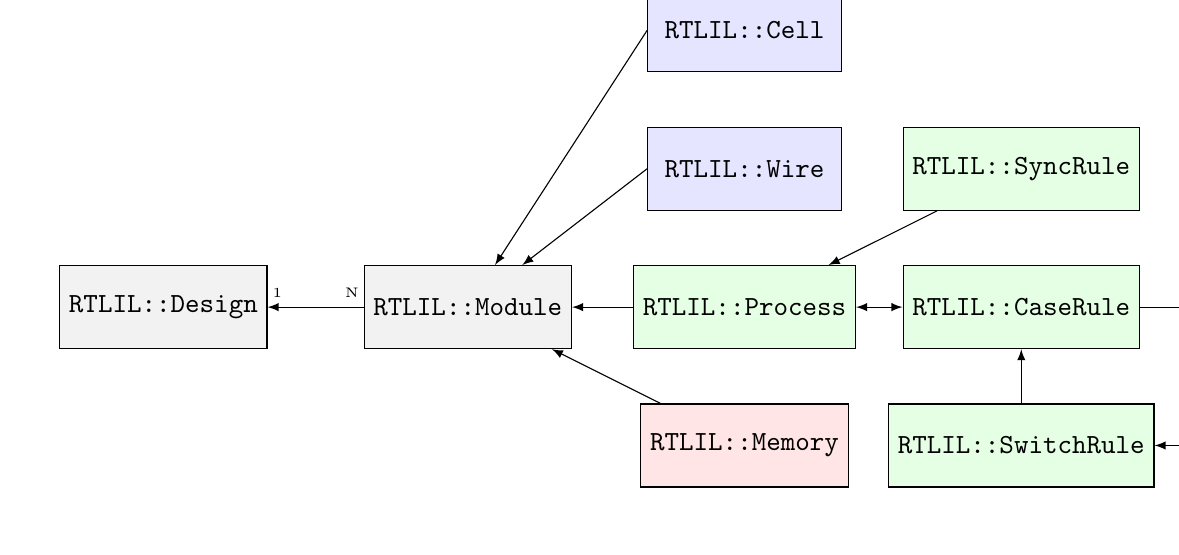
\begin{tikzpicture}
		\tikzstyle{entity} = [draw, fill=gray!10, rectangle, minimum height=3em, minimum width=7em, node distance=5em, font={\ttfamily}]
		\node[entity] (design) {RTLIL::Design};
		\node[entity] (module) [right of=design, node distance=11em] {RTLIL::Module} edge [-latex] node[above] {\tiny 1 \hskip3em N} (design);

		\node[entity] (process) [fill=green!10, right of=module, node distance=10em] {RTLIL::Process} (process.west) edge [-latex] (module);
		\node[entity] (memory) [fill=red!10, below of=process] {RTLIL::Memory} edge [-latex] (module);
		\node[entity] (wire) [fill=blue!10, above of=process] {RTLIL::Wire} (wire.west) edge [-latex] (module);
		\node[entity] (cell) [fill=blue!10, above of=wire] {RTLIL::Cell} (cell.west) edge [-latex] (module);

		\node[entity] (case) [fill=green!10, right of=process, node distance=10em] {RTLIL::CaseRule} edge [latex-latex] (process);
		\node[entity] (sync) [fill=green!10, above of=case] {RTLIL::SyncRule} edge [-latex] (process);
		\node[entity] (switch) [fill=green!10, below of=case] {RTLIL::SwitchRule} edge [-latex] (case);
		\draw[latex-] (switch.east) -- ++(1em,0) |- (case.east);
	\end{tikzpicture}
	\caption{Simplified RTLIL Entity-Relationship Diagram}
	\label{fig:Overview_RTLIL}
\end{figure}

There is only one active RTLIL::Design object that is used by all frontends,
passes and backends called by the user, e.g.~using a synthesis script. The RTLIL::Design then contains
zero to many RTLIL::Module objects. This corresponds to modules in Verilog or entities in VHDL. Each
module in turn contains objects from three different categories:

\begin{itemize}
\item RTLIL::Cell and RTLIL::Wire objects represent classical netlist data.
\item RTLIL::Process objects represent the decision trees (if-then-else statements, etc.) and synchronization
declarations (clock signals and sensitivity) from Verilog {\tt always} and VHDL {\tt process} blocks.
\item RTLIL::Memory objects represent addressable memories (arrays).
\end{itemize}

\begin{sloppypar}
Usually the output of the synthesis procedure is a netlist, i.e. all
RTLIL::Process and RTLIL::Memory objects must be replaced by RTLIL::Cell and
RTLIL::Wire objects by synthesis passes.
\end{sloppypar}

All features of the HDL that cannot be mapped directly to these RTLIL classes must be
transformed to an RTLIL-compatible representation by the HDL frontend. This includes
Verilog-features such as generate-blocks, loops and parameters.

The following sections contain a more detailed description of the different
parts of RTLIL and rationale behind some of the design decisions.

\subsection{RTLIL Identifiers}

All identifiers in RTLIL (such as module names, port names, signal names, cell
types, etc.) follow the following naming convention: they must either start with
a backslash (\textbackslash) or a dollar sign (\$).

Identifiers starting with a backslash are public visible identifiers. Usually
they originate from one of the HDL input files. For example the signal name ``{\tt \textbackslash sig42}''
is most likely a signal that was declared using the name ``{\tt sig42}'' in an HDL input file.
On the other hand the signal name ``{\tt \$sig42}'' is an auto-generated signal name. The backends
convert all identifiers that start with a dollar sign to identifiers that do not collide with
identifiers that start with a backslash.

This has three advantages:

\begin{itemize}
\item First, it is impossible that an auto-generated identifier collides with
an identifier that was provided by the user.
\item Second, the information about which identifiers were originally
provided by the user is always available which can help guide some optimizations. For example the ``opt\_rmunused''
tries to preserve signals with a user-provided name but doesn't hesitate to delete signals that have
auto-generated names when they just duplicate other signals.
\item Third, the delicate job of finding suitable auto-generated public visible
names is deferred to one central location. Internally auto-generated names that
may hold important information for Yosys developers can be used without
disturbing external tools. For example the Verilog backend assigns names in the form {\tt \_{\it integer}\_}.
\end{itemize}

In order to avoid programming errors, the RTLIL data structures check if all
identifiers start with either a backslash or a dollar sign and generate a
runtime error if this rule is violated.

All RTLIL identifiers are case sensitive.

\subsection{RTLIL::Design and RTLIL::Module}

The RTLIL::Design object is basically just a container for RTLIL::Module objects. In addition to
a list of RTLIL::Module objects the RTLIL::Design also keeps a list of {\it selected objects}, i.e.
the objects that passes should operate on. In most cases the whole design is selected and therefore
passes operate on the whole design. But this mechanism can be useful for more complex synthesis jobs
in which only parts of the design should be affected by certain passes.

Besides the objects shown in the ER diagram in Fig.~\ref{fig:Overview_RTLIL} an RTLIL::Module object
contains the following additional properties:

\begin{itemize}
\item The module name
\item A list of attributes
\item A list of connections between wires
\item An optional frontend callback used to derive parametrized variations of the module
\end{itemize}

The attributes can be Verilog attributes imported by the Verilog frontend or attributes assigned
by passes. They can be used to store additional metadata about modules or just mark them to be
used by certain part of the synthesis script but not by others.

Verilog and VHDL both support parametric modules (known as ``generic entities'' in VHDL). The RTLIL
format does not support parametric modules itself. Instead each module contains a callback function
into the AST frontend to generate a parametrized variation of the RTLIL::Module as needed. This
callback then returns the auto-generated name of the parametrized variation of the module. (A hash
over the parameters and the module name is used to prohibit the same parametrized variation from being
generated twice. For modules with only a few parameters, a name directly containing all parameters
is generated instead of a hash string.)

\subsection{RTLIL::Cell and RTLIL::Wire}

A module contains zero to many RTLIL::Cell and RTLIL::Wire objects. Objects of
these types are used to model netlists. Usually the goal of all synthesis efforts is to convert
all modules to a state where the functionality of the module is implemented only by cells
from a given cell library and wires to connect these cells with each other. Note that module
ports are just wires with a special property.

An RTLIL::Wire object has the following properties:

\begin{itemize}
\item The wire name
\item A list of attributes
\item A width (buses are just wires with a width > 1)
\item If the wire is a port: port number and direction (input/output/inout)
\end{itemize}

As with modules, the attributes can be Verilog attributes imported by the
Verilog frontend or attributes assigned by passes.

In Yosys, busses (signal vectors) are represented using a single wire object
with a width > 1. So Yosys does not convert signal vectors to individual signals.
This makes some aspects of RTLIL more complex but enables Yosys to be used for
coarse grain synthesis where the cells of the target architecture operate on
entire signal vectors instead of single bit wires.

An RTLIL::Cell object has the following properties:

\begin{itemize}
\item The cell name and type
\item A list of attributes
\item A list of parameters (for parametric cells)
\item Cell ports and the connections of ports to wires and constants
\end{itemize}

The connections of ports to wires are coded by assigning an RTLIL::SigSpec
to each cell port. The RTLIL::SigSpec data type is described in the next section.

\subsection{RTLIL::SigSpec}

A ``signal'' is everything that can be applied to a cell port. I.e.

\begin{itemize}
\item Any constant value of arbitrary bit-width \\
\null\hskip1em For example: \lstinline[language=Verilog]{1337, 16'b0000010100111001, 1'b1, 1'bx}
\item All bits of a wire or a selection of bits from a wire \\
\null\hskip1em For example: \lstinline[language=Verilog]{mywire, mywire[24], mywire[15:8]}
\item Concatenations of the above \\
\null\hskip1em For example: \lstinline[language=Verilog]|{16'd1337, mywire[15:8]}|
\end{itemize}

The RTLIL::SigSpec data type is used to represent signals. The RTLIL::Cell
object contains one RTLIL::SigSpec for each cell port.

In addition, connections between wires are represented using a pair of
RTLIL::SigSpec objects. Such pairs are needed in different locations. Therefore
the type name RTLIL::SigSig was defined for such a pair.

\subsection{RTLIL::Process}

When a high-level HDL frontend processes behavioural code it splits it up into
data path logic (e.g.~the expression {\tt a + b} is replaced by the output of an
adder that takes {\tt a} and {\tt b} as inputs) and an RTLIL::Process that models
the control logic of the behavioural code. Let's consider a simple example:

\begin{lstlisting}[numbers=left,frame=single,language=Verilog]
module ff_with_en_and_async_reset(clock, reset, enable, d, q);
input clock, reset, enable, d;
output reg q;
always @(posedge clock, posedge reset)
	if (reset)
		q <= 0;
	else if (enable)
		q <= d;
endmodule
\end{lstlisting}

In this example there is no data path and therefore the RTLIL::Module generated by
the frontend only contains a few RTLIL::Wire objects and an RTLIL::Process.
The RTLIL::Process in ILANG syntax:

\begin{lstlisting}[numbers=left,frame=single,language=rtlil]
process $proc$ff_with_en_and_async_reset.v:4$1
	assign $0\q[0:0] \q
	switch \reset
		case 1'1
			assign $0\q[0:0] 1'0
		case
			switch \enable
				case 1'1
					assign $0\q[0:0] \d
				case
			end
	end
	sync posedge \clock
		update \q $0\q[0:0]
	sync posedge \reset
		update \q $0\q[0:0]
end
\end{lstlisting}

This RTLIL::Process contains two RTLIL::SyncRule objects, two RTLIL::SwitchRule
objects and five RTLIL::CaseRule objects. The wire {\tt \$0\textbackslash{}q[0:0]}
is an automatically created wire that holds the next value of {\tt \textbackslash{}q}. The lines
$2 \dots 12$ describe how {\tt \$0\textbackslash{}q[0:0]} should be calculated. The
lines $13 \dots 16$ describe how the value of {\tt \$0\textbackslash{}q[0:0]} is used
to update {\tt \textbackslash{}q}.

An RTLIL::Process is a container for zero or more RTLIL::SyncRule objects and
exactly one RTLIL::CaseRule object, which is called the {\it root case}.

An RTLIL::SyncRule object contains an (optional) synchronization condition (signal and edge-type) and zero or
more assignments (RTLIL::SigSig). The {\tt always} synchronization condition is used to break combinatorial
loops when a latch should be inferred instead.

An RTLIL::CaseRule is a container for zero or more assignments (RTLIL::SigSig)
and zero or more RTLIL::SwitchRule objects. An RTLIL::SwitchRule objects is a
container for zero or more RTLIL::CaseRule objects.

In the above example the lines $2 \dots 12$ are the root case. Here {\tt \$0\textbackslash{}q[0:0]} is first
assigned the old value {\tt \textbackslash{}q} as default value (line 2). The root case
also contains an RTLIL::SwitchRule object (lines $3 \dots 12$). Such an object is very similar to the C {\tt switch}
statement as it uses a control signal ({\tt \textbackslash{}reset} in this case) to determine
which of its cases should be active. The RTLIL::SwitchRule object then contains one RTLIL::CaseRule
object per case. In this example there is a case\footnote{The
syntax {\tt 1'1} in the ILANG code specifies a constant with a length of one bit (the first ``1''),
and this bit is a one (the second ``1'').} for {\tt \textbackslash{}reset == 1} that causes
{\tt \$0\textbackslash{}q[0:0]} to be set (lines 4 and 5) and a default case that in turn contains a switch that
sets {\tt \$0\textbackslash{}q[0:0]} to the value of {\tt \textbackslash{}d} if {\tt
\textbackslash{}enable} is active (lines $6 \dots 11$).

A case can specify zero or more compare values that will determine whether it matches. Each of the compare values
must be the exact same width as the control signal. When more than one compare value is specified, the case matches
if any of them matches the control signal; when zero compare values are specified, the case always matches (i.e.
it is the default case).

A switch prioritizes cases from first to last: multiple cases can match, but only the first matched case becomes
active. This normally synthesizes to a priority encoder. The {\tt parallel\_case} attribute allows passes to assume
that no more than one case will match, and {\tt full\_case} attribute allows passes to assume that exactly one
case will match; if these invariants are ever dynamically violated, the behavior is undefined. These attributes
are useful when an invariant invisible to the synthesizer causes the control signal to never take certain
bit patterns.

The lines $13 \dots 16$  then cause {\tt \textbackslash{}q} to be updated whenever there is
a positive clock edge on {\tt \textbackslash{}clock} or {\tt \textbackslash{}reset}.

In order to generate such a representation, the language frontend must be able to handle blocking
and nonblocking assignments correctly. However, the language frontend does not need to identify
the correct type of storage element for the output signal or generate multiplexers for the
decision tree. This is done by passes that work on the RTLIL representation. Therefore it is
relatively easy to substitute these steps with other algorithms that target different target
architectures or perform optimizations or other transformations on the decision trees before
further processing them.

One of the first actions performed on a design in RTLIL representation in most
synthesis scripts is identifying asynchronous resets. This is usually done using the {\tt proc\_arst}
pass. This pass transforms the above example to the following RTLIL::Process:

\begin{lstlisting}[numbers=left,frame=single,language=rtlil]
process $proc$ff_with_en_and_async_reset.v:4$1
	assign $0\q[0:0] \q
	switch \enable
		case 1'1
			assign $0\q[0:0] \d
		case
	end
	sync posedge \clock
		update \q $0\q[0:0]
	sync high \reset
		update \q 1'0
end
\end{lstlisting}

This pass has transformed the outer RTLIL::SwitchRule into a modified RTLIL::SyncRule object
for the {\tt \textbackslash{}reset} signal. Further processing converts the RTLIL::Process
into e.g.~a d-type flip-flop with asynchronous reset and a multiplexer for the enable signal:

\begin{lstlisting}[numbers=left,frame=single,language=rtlil]
cell $adff $procdff$6
	parameter \ARST_POLARITY 1'1
	parameter \ARST_VALUE 1'0
	parameter \CLK_POLARITY 1'1
	parameter \WIDTH 1
	connect \ARST \reset
	connect \CLK \clock
	connect \D $0\q[0:0]
	connect \Q \q
end
cell $mux $procmux$3
	parameter \WIDTH 1
	connect \A \q
	connect \B \d
	connect \S \enable
	connect \Y $0\q[0:0]
end
\end{lstlisting}

Different combinations of passes may yield different results. Note that {\tt \$adff} and {\tt
\$mux} are internal cell types that still need to be mapped to cell types from the
target cell library.

Some passes refuse to operate on modules that still contain RTLIL::Process objects as the
presence of these objects in a module increases the complexity. Therefore the passes to translate
processes to a netlist of cells are usually called early in a synthesis script. The {\tt proc}
pass calls a series of other passes that together perform this conversion in a way that is suitable
for most synthesis tasks.

\subsection{RTLIL::Memory}

For every array (memory) in the HDL code an RTLIL::Memory object is created. A
memory object has the following properties:

\begin{itemize}
\item The memory name
\item A list of attributes
\item The width of an addressable word
\item The size of the memory in number of words
\end{itemize}

All read accesses to the memory are transformed to {\tt \$memrd} cells and all write accesses to
{\tt \$memwr} cells by the language frontend. These cells consist of independent read- and write-ports
to the memory. Memory initialization is transformed to {\tt \$meminit} cells by the language frontend.
The \B{MEMID} parameter on these cells is used to link them together and to the RTLIL::Memory object they belong to.

The rationale behind using separate cells for the individual ports versus
creating a large multiport memory cell right in the language frontend is that
the separate {\tt \$memrd} and {\tt \$memwr} cells can be consolidated using resource sharing.
As resource sharing is a non-trivial optimization problem where different synthesis tasks
can have different requirements it lends itself to do the optimisation in separate passes and merge
the RTLIL::Memory objects and {\tt \$memrd} and {\tt \$memwr} cells to multiport memory blocks after resource sharing is completed.

The {\tt memory} pass performs this conversion and can (depending on the options passed
to it) transform the memories directly to d-type flip-flops and address logic or yield
multiport memory blocks (represented using {\tt \$mem} cells).

See Sec.~\ref{sec:memcells} for details about the memory cell types.

\section{Command Interface and Synthesis Scripts}

Yosys reads and processes commands from synthesis scripts, command line arguments and
an interactive command prompt. Yosys commands consist of a command name and an optional
whitespace separated list of arguments. Commands are terminated using the newline character
or a semicolon ({\tt ;}). Empty lines and lines starting with the hash sign ({\tt \#}) are ignored.
See Sec.~\ref{sec:typusecase} for an example synthesis script.

The command {\tt help} can be used to access the command reference manual.

Most commands can operate not only on the entire design but also specifically on {\it selected}
parts of the design. For example the command {\tt dump} will print all selected objects
in the current design while {\tt dump foobar} will only print the module {\tt foobar}
and {\tt dump *} will print the entire design regardless of the current selection.

The selection mechanism is very powerful. For example the command {\tt dump */t:\$add
\%x:+[A] */w:* \%i} will print all wires that are connected to the \B{A} port of
a {\tt \$add} cell.  Detailed documentation of the select framework can be
found in the command reference for the {\tt select} command.

\section{Source Tree and Build System}

The Yosys source tree is organized into the following top-level directories:

\begin{itemize}

\item {\tt backends/} \\
This directory contains a subdirectory for each of the backend modules.

\item {\tt frontends/} \\
This directory contains a subdirectory for each of the frontend modules.

\item {\tt kernel/} \\
This directory contains all the core functionality of Yosys. This includes the
functions and definitions for working with the RTLIL data structures ({\tt
rtlil.h} and {\tt rtlil.cc}), the main() function ({\tt driver.cc}), the
internal framework for generating log messages ({\tt log.h} and {\tt log.cc}),
the internal framework for registering and calling passes ({\tt register.h} and
{\tt register.cc}), some core commands that are not really passes ({\tt
select.cc}, {\tt show.cc}, \dots) and a couple of other small utility libraries.

\item {\tt passes/} \\
This directory contains a subdirectory for each pass or group of passes. For example as
of this writing the directory {\tt passes/opt/} contains the code for seven
passes: {\tt opt}, {\tt opt\_expr}, {\tt opt\_muxtree}, {\tt opt\_reduce},
{\tt opt\_rmdff}, {\tt opt\_rmunused} and {\tt opt\_merge}.

\item {\tt techlibs/} \\
This directory contains simulation models and standard implementations for the
cells from the internal cell library.

\item {\tt tests/} \\
This directory contains a couple of test cases. Most of the smaller tests are executed
automatically when {\tt make test} is called. The larger tests must be executed
manually. Most of the larger tests require downloading external HDL source code
and/or external tools. The tests range from comparing simulation results of the synthesized
design to the original sources to logic equivalence checking of entire CPU cores.

\end{itemize}

\begin{sloppypar}
The top-level Makefile includes {\tt frontends/*/Makefile.inc}, {\tt passes/*/Makefile.inc}
and {\tt backends/*/Makefile.inc}. So when extending Yosys it is enough to create
a new directory in {\tt frontends/}, {\tt passes/} or {\tt backends/} with your sources
and a {\tt Makefile.inc}. The Yosys kernel automatically detects all commands linked with
Yosys. So it is not needed to add additional commands to a central list of commands.
\end{sloppypar}

Good starting points for reading example source code to learn how to write passes
are {\tt passes/opt/opt\_rmdff.cc} and {\tt passes/opt/opt\_merge.cc}.

See the top-level README file for a quick {\it Getting Started} guide and build
instructions. The Yosys build is based solely on Makefiles.

Users of the Qt Creator IDE can generate a QT Creator project file using {\tt
make qtcreator}. Users of the Eclipse IDE can use the ``Makefile Project with
Existing Code'' project type in the Eclipse ``New Project'' dialog (only
available after the CDT plugin has been installed) to create an Eclipse project
in order to programming extensions to Yosys or just browse the Yosys code base.



\chapter{Internal Cell Library}
\label{chapter:celllib}

Most of the passes in Yosys operate on netlists, i.e.~they only care about the RTLIL::Wire and RTLIL::Cell
objects in an RTLIL::Module. This chapter discusses the cell types used by Yosys to represent a behavioural
design internally.

This chapter is split in two parts. In the first part the internal RTL cells are covered. These cells
are used to represent the design on a coarse grain level. Like in the original HDL code on this level the
cells operate on vectors of signals and complex cells like adders exist. In the second part the internal
gate cells are covered. These cells are used to represent the design on a fine-grain gate-level. All cells
from this category operate on single bit signals.

\section{RTL Cells}

Most of the RTL cells closely resemble the operators available in HDLs such as
Verilog or VHDL. Therefore Verilog operators are used in the following sections
to define the behaviour of the RTL cells.

Note that all RTL cells have parameters indicating the size of inputs and outputs. When
passes modify RTL cells they must always keep the values of these parameters in sync with
the size of the signals connected to the inputs and outputs.

Simulation models for the RTL cells can be found in the file {\tt techlibs/common/simlib.v} in the Yosys
source tree.

\subsection{Unary Operators}

All unary RTL cells have one input port \B{A} and one output port \B{Y}. They also
have the following parameters:

\begin{itemize}
\item \B{A\_SIGNED} \\
Set to a non-zero value if the input \B{A} is signed and therefore should be sign-extended
when needed.

\item \B{A\_WIDTH} \\
The width of the input port \B{A}.

\item \B{Y\_WIDTH} \\
The width of the output port \B{Y}.
\end{itemize}

Table~\ref{tab:CellLib_unary} lists all cells for unary RTL operators.

\begin{table}[t!]
\hfil
\begin{tabular}{ll}
Verilog & Cell Type \\
\hline
\lstinline[language=Verilog]; Y =  ~A ; & {\tt \$not} \\
\lstinline[language=Verilog]; Y =  +A ; & {\tt \$pos} \\
\lstinline[language=Verilog]; Y =  -A ; & {\tt \$neg} \\
\hline
\lstinline[language=Verilog]; Y =  &A ; & {\tt \$reduce\_and} \\
\lstinline[language=Verilog]; Y =  |A ; & {\tt \$reduce\_or} \\
\lstinline[language=Verilog]; Y =  ^A ; & {\tt \$reduce\_xor} \\
\lstinline[language=Verilog]; Y = ~^A ; & {\tt \$reduce\_xnor} \\
\hline
\lstinline[language=Verilog]; Y =  |A ; & {\tt \$reduce\_bool} \\
\lstinline[language=Verilog]; Y =  !A ; & {\tt \$logic\_not}
\end{tabular}
\caption{Cell types for unary operators with their corresponding Verilog expressions.}
\label{tab:CellLib_unary}
\end{table}

Note that {\tt \$reduce\_or} and {\tt \$reduce\_bool} actually represent the same
logic function. But the HDL frontends generate them in different situations. A
{\tt \$reduce\_or} cell is generated when the prefix {\tt |} operator is being used. A
{\tt \$reduce\_bool} cell is generated when a bit vector is used as a condition in
an {\tt if}-statement or {\tt ?:}-expression.

\subsection{Binary Operators}

All binary RTL cells have two input ports \B{A} and \B{B} and one output port \B{Y}. They
also have the following parameters:

\begin{itemize}
\item \B{A\_SIGNED} \\
Set to a non-zero value if the input \B{A} is signed and therefore should be sign-extended
when needed.

\item \B{A\_WIDTH} \\
The width of the input port \B{A}.

\item \B{B\_SIGNED} \\
Set to a non-zero value if the input \B{B} is signed and therefore should be sign-extended
when needed.

\item \B{B\_WIDTH} \\
The width of the input port \B{B}.

\item \B{Y\_WIDTH} \\
The width of the output port \B{Y}.
\end{itemize}

Table~\ref{tab:CellLib_binary} lists all cells for binary RTL operators.

\subsection{Multiplexers}

Multiplexers are generated by the Verilog HDL frontend for {\tt
?:}-expressions. Multiplexers are also generated by the {\tt proc} pass to map the decision trees
from RTLIL::Process objects to logic.

The simplest multiplexer cell type is {\tt \$mux}. Cells of this type have a \B{WIDTH} parameter
and data inputs \B{A} and \B{B} and a data output \B{Y}, all of the specified width. This cell also
has a single bit control input \B{S}. If \B{S} is 0 the value from the \B{A} input is sent to
the output, if it is 1 the value from the \B{B} input is sent to the output. So the {\tt \$mux}
cell implements the function \lstinline[language=Verilog]; Y = S ? B : A;.

The {\tt \$pmux} cell is used to multiplex between many inputs using a one-hot select signal. Cells
of this type have a \B{WIDTH} and a \B{S\_WIDTH} parameter and inputs \B{A}, \B{B}, and \B{S} and
an output \B{Y}. The \B{S} input is \B{S\_WIDTH} bits wide. The \B{A} input and the output are both
\B{WIDTH} bits wide and the \B{B} input is \B{WIDTH}*\B{S\_WIDTH} bits wide. When all bits of
\B{S} are zero, the value from \B{A} input is sent to the output. If the $n$'th bit from \B{S} is
set, the value $n$'th \B{WIDTH} bits wide slice of the \B{B} input is sent to the output. When more
than one bit from \B{S} is set the output is undefined. Cells of this type are used to model
``parallel cases'' (defined by using the {\tt parallel\_case} attribute or detected by
an optimization).

The {\tt \$tribuf} cell is used to implement tristate logic. Cells of this type have a \B{WIDTH}
parameter and inputs \B{A} and \B{EN} and an output \B{Y}. The \B{A} input and \B{Y} output are
\B{WIDTH} bits wide, and the \B{EN} input is one bit wide. When \B{EN} is 0, the output \B{Y}
is not driven. When \B{EN} is 1, the value from \B{A} input is sent to the \B{Y} output. Therefore,
the {\tt \$tribuf} cell implements the function \lstinline[language=Verilog]; Y = EN ? A : 'bz;.

Behavioural code with cascaded {\tt if-then-else}- and {\tt case}-statements
usually results in trees of multiplexer cells. Many passes (from various
optimizations to FSM extraction) heavily depend on these multiplexer trees to
understand dependencies between signals. Therefore optimizations should not
break these multiplexer trees (e.g.~by replacing a multiplexer between a
calculated signal and a constant zero with an {\tt \$and} gate).

\begin{table}[t!]
\hfil
\begin{tabular}[t]{ll}
Verilog & Cell Type \\
\hline
\lstinline[language=Verilog]; Y = A  & B; & {\tt \$and} \\
\lstinline[language=Verilog]; Y = A  | B; & {\tt \$or} \\
\lstinline[language=Verilog]; Y = A  ^ B; & {\tt \$xor} \\
\lstinline[language=Verilog]; Y = A ~^ B; & {\tt \$xnor} \\
\hline
\lstinline[language=Verilog]; Y = A << B; & {\tt \$shl} \\
\lstinline[language=Verilog]; Y = A >> B; & {\tt \$shr} \\
\lstinline[language=Verilog]; Y = A <<< B; & {\tt \$sshl} \\
\lstinline[language=Verilog]; Y = A >>> B; & {\tt \$sshr} \\
\hline
\lstinline[language=Verilog]; Y = A && B; & {\tt \$logic\_and} \\
\lstinline[language=Verilog]; Y = A || B; & {\tt \$logic\_or} \\
\hline
\lstinline[language=Verilog]; Y = A === B; & {\tt \$eqx} \\
\lstinline[language=Verilog]; Y = A !== B; & {\tt \$nex} \\
\end{tabular}
\hfil
\begin{tabular}[t]{ll}
Verilog & Cell Type \\
\hline
\lstinline[language=Verilog]; Y = A <  B; & {\tt \$lt} \\
\lstinline[language=Verilog]; Y = A <= B; & {\tt \$le} \\
\lstinline[language=Verilog]; Y = A == B; & {\tt \$eq} \\
\lstinline[language=Verilog]; Y = A != B; & {\tt \$ne} \\
\lstinline[language=Verilog]; Y = A >= B; & {\tt \$ge} \\
\lstinline[language=Verilog]; Y = A >  B; & {\tt \$gt} \\
\hline
\lstinline[language=Verilog]; Y = A  + B; & {\tt \$add} \\
\lstinline[language=Verilog]; Y = A  - B; & {\tt \$sub} \\
\lstinline[language=Verilog]; Y = A  * B; & {\tt \$mul} \\
\lstinline[language=Verilog]; Y = A  / B; & {\tt \$div} \\
\lstinline[language=Verilog]; Y = A  % B; & {\tt \$mod} \\
\lstinline[language=Verilog]; Y = A ** B; & {\tt \$pow} \\
\end{tabular}
\caption{Cell types for binary operators with their corresponding Verilog expressions.}
\label{tab:CellLib_binary}
\end{table}

\subsection{Registers}

D-Type Flip-Flops are represented by {\tt \$dff} cells. These cells have a clock port \B{CLK},
an input port \B{D} and an output port \B{Q}. The following parameters are available for \$dff
cells:

\begin{itemize}
\item \B{WIDTH} \\
The width of input \B{D} and output \B{Q}.

\item \B{CLK\_POLARITY} \\
Clock is active on the positive edge if this parameter has the value {\tt 1'b1} and on the negative
edge if this parameter is {\tt 1'b0}.
\end{itemize}

D-Type Flip-Flops with asynchronous resets are represented by {\tt \$adff} cells. As the {\tt \$dff}
cells they have \B{CLK}, \B{D} and \B{Q} ports. In addition they also have a single-bit \B{ARST}
input port for the reset pin and the following additional two parameters:

\begin{itemize}
\item \B{ARST\_POLARITY} \\
The asynchronous reset is high-active if this parameter has the value {\tt 1'b1} and low-active
if this parameter is {\tt 1'b0}.

\item \B{ARST\_VALUE} \\
The state of \B{Q} will be set to this value when the reset is active.
\end{itemize}

Note that the {\tt \$adff} cell can only be used when the reset value is constant.

\begin{sloppypar}
Usually these cells are generated by the {\tt proc} pass using the information
in the designs RTLIL::Process objects.
\end{sloppypar}

\begin{fixme}
Add information about {\tt \$sr} cells (set-reset flip-flops) and d-type latches.
\end{fixme}

\subsection{Memories}
\label{sec:memcells}

Memories are either represented using RTLIL::Memory objects, {\tt \$memrd}, {\tt \$memwr}, and {\tt \$meminit}
cells, or by {\tt \$mem} cells alone.

In the first alternative the RTLIL::Memory objects hold the general metadata for the memory (bit width,
size in number of words, etc.) and for each port a {\tt \$memrd} (read port) or {\tt \$memwr} (write port)
cell is created. Having individual cells for read and write ports has the advantage that they can be
consolidated using resource sharing passes. In some cases this drastically reduces the number of required
ports on the memory cell. In this alternative, memory initialization data is represented by {\tt \$meminit} cells,
which allow delaying constant folding for initialization addresses and data until after the frontend finishes.

The {\tt \$memrd} cells have a clock input \B{CLK}, an enable input \B{EN}, an
address input \B{ADDR}, and a data output \B{DATA}. They also have the
following parameters:

\begin{itemize}
\item \B{MEMID} \\
The name of the RTLIL::Memory object that is associated with this read port.

\item \B{ABITS} \\
The number of address bits (width of the \B{ADDR} input port).

\item \B{WIDTH} \\
The number of data bits (width of the \B{DATA} output port).

\item \B{CLK\_ENABLE} \\
When this parameter is non-zero, the clock is used. Otherwise this read port is asynchronous and
the \B{CLK} input is not used.

\item \B{CLK\_POLARITY} \\
Clock is active on the positive edge if this parameter has the value {\tt 1'b1} and on the negative
edge if this parameter is {\tt 1'b0}.

\item \B{TRANSPARENT} \\
If this parameter is set to {\tt 1'b1}, a read and write to the same address in the same cycle will
return the new value. Otherwise the old value is returned.
\end{itemize}

The {\tt \$memwr} cells have a clock input \B{CLK}, an enable input \B{EN} (one
enable bit for each data bit), an address input \B{ADDR} and a data input
\B{DATA}. They also have the following parameters:

\begin{itemize}
\item \B{MEMID} \\
The name of the RTLIL::Memory object that is associated with this write port.

\item \B{ABITS} \\
The number of address bits (width of the \B{ADDR} input port).

\item \B{WIDTH} \\
The number of data bits (width of the \B{DATA} output port).

\item \B{CLK\_ENABLE} \\
When this parameter is non-zero, the clock is used. Otherwise this write port is asynchronous and
the \B{CLK} input is not used.

\item \B{CLK\_POLARITY} \\
Clock is active on positive edge if this parameter has the value {\tt 1'b1} and on the negative
edge if this parameter is {\tt 1'b0}.

\item \B{PRIORITY} \\
The cell with the higher integer value in this parameter wins a write conflict.
\end{itemize}

The {\tt \$meminit} cells have an address input \B{ADDR} and a data input \B{DATA}, with the width
of the \B{DATA} port equal to \B{WIDTH} parameter times \B{WORDS} parameter. Both of the inputs
must resolve to a constant for synthesis to succeed.

\begin{itemize}
\item \B{MEMID} \\
The name of the RTLIL::Memory object that is associated with this initialization cell.

\item \B{ABITS} \\
The number of address bits (width of the \B{ADDR} input port).

\item \B{WIDTH} \\
The number of data bits per memory location.

\item \B{WORDS} \\
The number of consecutive memory locations initialized by this cell.

\item \B{PRIORITY} \\
The cell with the higher integer value in this parameter wins an initialization conflict.
\end{itemize}

The HDL frontend models a memory using RTLIL::Memory objects and asynchronous
{\tt \$memrd} and {\tt \$memwr} cells. The {\tt memory} pass (i.e.~its various sub-passes) migrates
{\tt \$dff} cells into the {\tt \$memrd} and {\tt \$memwr} cells making them synchronous, then
converts them to a single {\tt \$mem} cell and (optionally) maps this cell type
to {\tt \$dff} cells for the individual words and multiplexer-based address decoders for the read and
write interfaces. When the last step is disabled or not possible, a {\tt \$mem} cell is left in the design.

The {\tt \$mem} cell provides the following parameters:

\begin{itemize}
\item \B{MEMID} \\
The name of the original RTLIL::Memory object that became this {\tt \$mem} cell.

\item \B{SIZE} \\
The number of words in the memory.

\item \B{ABITS} \\
The number of address bits.

\item \B{WIDTH} \\
The number of data bits per word.

\item \B{INIT} \\
The initial memory contents.

\item \B{RD\_PORTS} \\
The number of read ports on this memory cell.

\item \B{RD\_CLK\_ENABLE} \\
This parameter is \B{RD\_PORTS} bits wide, containing a clock enable bit for each read port.

\item \B{RD\_CLK\_POLARITY} \\
This parameter is \B{RD\_PORTS} bits wide, containing a clock polarity bit for each read port.

\item \B{RD\_TRANSPARENT} \\
This parameter is \B{RD\_PORTS} bits wide, containing a transparent bit for each read port.

\item \B{WR\_PORTS} \\
The number of write ports on this memory cell.

\item \B{WR\_CLK\_ENABLE} \\
This parameter is \B{WR\_PORTS} bits wide, containing a clock enable bit for each write port.

\item \B{WR\_CLK\_POLARITY} \\
This parameter is \B{WR\_PORTS} bits wide, containing a clock polarity bit for each write port.
\end{itemize}

The {\tt \$mem} cell has the following ports:

\begin{itemize}
\item \B{RD\_CLK} \\
This input is \B{RD\_PORTS} bits wide, containing all clock signals for the read ports.

\item \B{RD\_EN} \\
This input is \B{RD\_PORTS} bits wide, containing all enable signals for the read ports.

\item \B{RD\_ADDR} \\
This input is \B{RD\_PORTS}*\B{ABITS} bits wide, containing all address signals for the read ports.

\item \B{RD\_DATA} \\
This input is \B{RD\_PORTS}*\B{WIDTH} bits wide, containing all data signals for the read ports.

\item \B{WR\_CLK} \\
This input is \B{WR\_PORTS} bits wide, containing all clock signals for the write ports.

\item \B{WR\_EN} \\
This input is \B{WR\_PORTS}*\B{WIDTH} bits wide, containing all enable signals for the write ports.

\item \B{WR\_ADDR} \\
This input is \B{WR\_PORTS}*\B{ABITS} bits wide, containing all address signals for the write ports.

\item \B{WR\_DATA} \\
This input is \B{WR\_PORTS}*\B{WIDTH} bits wide, containing all data signals for the write ports.
\end{itemize}

The {\tt memory\_collect} pass can be used to convert discrete {\tt \$memrd}, {\tt \$memwr}, and {\tt \$meminit} cells
belonging to the same memory to a single {\tt \$mem} cell, whereas the {\tt memory\_unpack} pass performs the inverse operation.
The {\tt memory\_dff} pass can combine asynchronous memory ports that are fed by or feeding registers into synchronous memory ports.
The {\tt memory\_bram} pass can be used to recognize {\tt \$mem} cells that can be implemented with a block RAM resource on an FPGA.
The {\tt memory\_map} pass can be used to implement {\tt \$mem} cells as basic logic: word-wide DFFs and address decoders.

\subsection{Finite State Machines}

\begin{fixme}
Add a brief description of the {\tt \$fsm} cell type.
\end{fixme}

\section{Gates}
\label{sec:celllib_gates}

For gate level logic networks, fixed function single bit cells are used that do
not provide any parameters.

Simulation models for these cells can be found in the file {\tt techlibs/common/simcells.v} in the Yosys
source tree.

\begin{table}[t]
\hfil
\begin{tabular}[t]{ll}
Verilog & Cell Type \\
\hline
\lstinline[language=Verilog]; Y = ~A;    & {\tt \$\_NOT\_} \\
\lstinline[language=Verilog]; Y = A & B; & {\tt \$\_AND\_} \\
\lstinline[language=Verilog]; Y = ~(A & B); & {\tt \$\_NAND\_} \\
\lstinline[language=Verilog]; Y = A & ~B; & {\tt \$\_ANDNOT\_} \\
\lstinline[language=Verilog]; Y = A | B; & {\tt \$\_OR\_} \\
\lstinline[language=Verilog]; Y = ~(A | B); & {\tt \$\_NOR\_} \\
\lstinline[language=Verilog]; Y = A | ~B; & {\tt \$\_ORNOT\_} \\
\lstinline[language=Verilog]; Y = A ^ B; & {\tt \$\_XOR\_} \\
\lstinline[language=Verilog]; Y = ~(A ^ B); & {\tt \$\_XNOR\_} \\
\lstinline[language=Verilog]; Y = S ? B : A; & {\tt \$\_MUX\_} \\
\lstinline[language=Verilog]; Y = EN ? A : 'bz; & {\tt \$\_TBUF\_} \\
\hline
\lstinline[language=Verilog]; always @(negedge C) Q <= D; & {\tt \$\_DFF\_N\_} \\
\lstinline[language=Verilog]; always @(posedge C) Q <= D; & {\tt \$\_DFF\_P\_} \\
\end{tabular}
\hfil
\begin{tabular}[t]{llll}
$ClkEdge$ & $RstLvl$ & $RstVal$ & Cell Type \\
\hline
\lstinline[language=Verilog];negedge; & \lstinline[language=Verilog];0; & \lstinline[language=Verilog];0; & {\tt \$\_DFF\_NN0\_} \\
\lstinline[language=Verilog];negedge; & \lstinline[language=Verilog];0; & \lstinline[language=Verilog];1; & {\tt \$\_DFF\_NN1\_} \\
\lstinline[language=Verilog];negedge; & \lstinline[language=Verilog];1; & \lstinline[language=Verilog];0; & {\tt \$\_DFF\_NP0\_} \\
\lstinline[language=Verilog];negedge; & \lstinline[language=Verilog];1; & \lstinline[language=Verilog];1; & {\tt \$\_DFF\_NP1\_} \\
\lstinline[language=Verilog];posedge; & \lstinline[language=Verilog];0; & \lstinline[language=Verilog];0; & {\tt \$\_DFF\_PN0\_} \\
\lstinline[language=Verilog];posedge; & \lstinline[language=Verilog];0; & \lstinline[language=Verilog];1; & {\tt \$\_DFF\_PN1\_} \\
\lstinline[language=Verilog];posedge; & \lstinline[language=Verilog];1; & \lstinline[language=Verilog];0; & {\tt \$\_DFF\_PP0\_} \\
\lstinline[language=Verilog];posedge; & \lstinline[language=Verilog];1; & \lstinline[language=Verilog];1; & {\tt \$\_DFF\_PP1\_} \\
\end{tabular}
\caption{Cell types for gate level logic networks}
\label{tab:CellLib_gates}
\end{table}

Table~\ref{tab:CellLib_gates} lists all cell types used for gate level logic. The cell types
{\tt \$\_NOT\_}, {\tt \$\_AND\_}, {\tt \$\_NAND\_}, {\tt \$\_ANDNOT\_}, {\tt \$\_OR\_}, {\tt \$\_NOR\_},
{\tt \$\_ORNOT\_}, {\tt \$\_XOR\_}, {\tt \$\_XNOR\_} and {\tt \$\_MUX\_} are used to model combinatorial logic.
The cell type {\tt \$\_TBUF\_} is used to model tristate logic.
The cell types {\tt \$\_DFF\_N\_} and {\tt \$\_DFF\_P\_} represent d-type flip-flops.

The cell types {\tt \$\_DFF\_NN0\_}, {\tt \$\_DFF\_NN1\_}, {\tt \$\_DFF\_NP0\_}, {\tt \$\_DFF\_NP1\_},
{\tt \$\_DFF\_PN0\_}, {\tt \$\_DFF\_PN1\_}, {\tt \$\_DFF\_PP0\_} and {\tt \$\_DFF\_PP1\_} implement
d-type flip-flops with asynchronous resets. The values in the table for these cell types relate to the
following Verilog code template, where \lstinline[mathescape,language=Verilog];$RstEdge$; is \lstinline[language=Verilog];posedge;
if \lstinline[mathescape,language=Verilog];$RstLvl$; if \lstinline[language=Verilog];1;, and \lstinline[language=Verilog];negedge;
otherwise.

\begin{lstlisting}[mathescape,language=Verilog]
	always @($ClkEdge$ C, $RstEdge$ R)
		if (R == $RstLvl$)
			Q <= $RstVal$;
		else
			Q <= D;
\end{lstlisting}

In most cases gate level logic networks are created from RTL networks using the {\tt techmap} pass. The flip-flop cells
from the gate level logic network can be mapped to physical flip-flop cells from a Liberty file using the {\tt dfflibmap}
pass. The combinatorial logic cells can be mapped to physical cells from a Liberty file via ABC \citeweblink{ABC}
using the {\tt abc} pass.

\begin{fixme}
Add information about {\tt \$assert}, {\tt \$assume}, {\tt \$live}, {\tt \$fair}, {\tt \$cover}, {\tt \$equiv},
{\tt \$initstate}, {\tt \$anyconst}, {\tt \$anyseq}, {\tt \$allconst}, {\tt \$allseq} cells.
\end{fixme}

\begin{fixme}
Add information about {\tt \$specify2}, {\tt \$specify3}, and {\tt \$specrule} cells.
\end{fixme}

\begin{fixme}
Add information about {\tt \$slice} and {\tt \$concat} cells.
\end{fixme}

\begin{fixme}
Add information about {\tt \$lut} and {\tt \$sop} cells.
\end{fixme}

\begin{fixme}
Add information about {\tt \$alu}, {\tt \$macc}, {\tt \$fa}, and {\tt \$lcu} cells.
\end{fixme}

\begin{fixme}
Add information about {\tt \$ff} and {\tt \$\_FF\_} cells.
\end{fixme}

\begin{fixme}
Add information about {\tt \$dffe}, {\tt \$dffsr}, {\tt \$dlatch}, and {\tt \$dlatchsr} cells.
\end{fixme}

\begin{fixme}
Add information about {\tt \$\_DFFE\_??\_}, {\tt \$\_DFFSR\_???\_}, {\tt \$\_DLATCH\_?\_}, and {\tt \$\_DLATCHSR\_???\_} cells.
\end{fixme}

\begin{fixme}
Add information about {\tt \$\_AOI3\_}, {\tt \$\_OAI3\_}, {\tt \$\_AOI4\_}, {\tt \$\_OAI4\_}, and {\tt \$\_NMUX\_} cells.
\end{fixme}



\chapter{Programming Yosys Extensions}
\label{chapter:prog}

This chapter contains some bits and pieces of information about programming
yosys extensions. Also consult the section on programming in the ``Yosys
Presentation'' (can be downloaded from the Yosys website as PDF) and don't
be afraid to ask questions on the Yosys Subreddit.

\section{The ``CodingReadme'' File}

The following is an excerpt of the {\tt CodingReadme} file from the Yosys source tree.

\lstinputlisting[title=CodingReadme,rangeprefix=--,rangesuffix=--,includerangemarker=false,linerange=snip-snap,numbers=left,frame=single]{../CodingReadme}

\section{The ``stubsnets'' Example Module}

The following is the complete code of the ``stubsnets'' example module. It is included in the Yosys source distribution as {\tt manual/CHAPTER\_Prog/stubnets.cc}.


\lstinputlisting[title=stubnets.cc,numbers=left,frame=single,language=C++]{CHAPTER_Prog/stubnets.cc}

\lstinputlisting[title=Makefile,numbers=left,frame=single,language=make]{CHAPTER_Prog/Makefile}

\lstinputlisting[title=test.v,numbers=left,frame=single,language=Verilog]{CHAPTER_Prog/test.v}




\chapter{The Verilog and AST Frontends}
\label{chapter:verilog}

This chapter provides an overview of the implementation of the Yosys Verilog
and AST frontends. The Verilog frontend reads Verilog-2005 code and creates
an abstract syntax tree (AST) representation of the input. This AST representation
is then passed to the AST frontend that converts it to RTLIL data, as illustrated
in Fig.~\ref{fig:Verilog_flow}.

\begin{figure}[b!]
	\hfil
	\begin{tikzpicture}
		\tikzstyle{process} = [draw, fill=green!10, rectangle, minimum height=3em, minimum width=10em, node distance=5em, font={\ttfamily}]
		\tikzstyle{data} = [draw, fill=blue!10, ellipse, minimum height=3em, minimum width=7em, node distance=5em, font={\ttfamily}]

		\node[data]    (n1)               {Verilog Source};
		\node[process] (n2) [below of=n1] {Verilog Frontend};
		\node[data]    (n3) [below of=n2] {AST};
		\node[process] (n4) [below of=n3] {AST Frontend};
		\node[data]    (n5) [below of=n4] {RTLIL};

		\draw[-latex] (n1) -- (n2);
		\draw[-latex] (n2) -- (n3);
		\draw[-latex] (n3) -- (n4);
		\draw[-latex] (n4) -- (n5);

		\tikzstyle{details} = [draw, fill=yellow!5, rectangle, node distance=6cm, font={\ttfamily}]

		\node[details] (d1) [right of=n2] {\begin{minipage}{5cm}
			\hfil
			\begin{tikzpicture}
				\tikzstyle{subproc} = [draw, fill=green!10, rectangle, minimum height=2em, minimum width=10em, node distance=3em, font={\ttfamily}]
				\node (s0) {};
				\node[subproc] (s1) [below of=s0] {Preprocessor};
				\node[subproc] (s2) [below of=s1] {Lexer};
				\node[subproc] (s3) [below of=s2] {Parser};
				\node[node distance=3em] (s4) [below of=s3] {};
				\draw[-latex] (s0) -- (s1);
				\draw[-latex] (s1) -- (s2);
				\draw[-latex] (s2) -- (s3);
				\draw[-latex] (s3) -- (s4);
			\end{tikzpicture}
		\end{minipage}};

		\draw[dashed] (n2.north east) -- (d1.north west);
		\draw[dashed] (n2.south east) -- (d1.south west);

		\node[details] (d2) [right of=n4] {\begin{minipage}{5cm}
			\hfil
			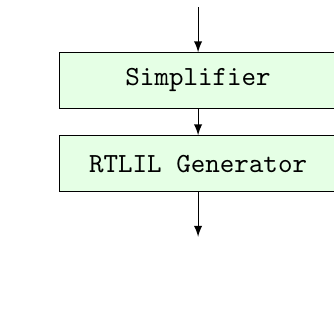
\begin{tikzpicture}
				\tikzstyle{subproc} = [draw, fill=green!10, rectangle, minimum height=2em, minimum width=10em, node distance=3em, font={\ttfamily}]
				\node (s0) {};
				\node[subproc] (s1) [below of=s0] {Simplifier};
				\node[subproc] (s2) [below of=s1] {RTLIL Generator};
				\node[node distance=3em] (s3) [below of=s2] {};
				\draw[-latex] (s0) -- (s1);
				\draw[-latex] (s1) -- (s2);
				\draw[-latex] (s2) -- (s3);
			\end{tikzpicture}
		\end{minipage}};

		\draw[dashed] (n4.north east) -- (d2.north west);
		\draw[dashed] (n4.south east) -- (d2.south west);

	\end{tikzpicture}
	\caption{Simplified Verilog to RTLIL data flow}
	\label{fig:Verilog_flow}
\end{figure}


\section{Transforming Verilog to AST}

The {\it Verilog frontend} converts the Verilog sources to an internal AST representation that closely resembles
the structure of the original Verilog code. The Verilog frontend consists of three components, the
{\it Preprocessor}, the {\it Lexer} and the {\it Parser}.

The source code to the Verilog frontend can be found in {\tt frontends/verilog/} in the Yosys source tree.

\subsection{The Verilog Preprocessor}

The Verilog preprocessor scans over the Verilog source code and interprets some of the Verilog compiler
directives such as \lstinline[language=Verilog]{`include}, \lstinline[language=Verilog]{`define} and
\lstinline[language=Verilog]{`ifdef}.

It is implemented as a C++ function that is passed a file descriptor as input and returns the
pre-processed Verilog code as a \lstinline[language=C++]{std::string}.

The source code to the Verilog Preprocessor can be found in {\tt
frontends/verilog/preproc.cc} in the Yosys source tree.

\subsection{The Verilog Lexer}

\begin{sloppypar}
The Verilog Lexer is written using the lexer generator {\it flex} \citeweblink{flex}. Its source code
can be found in {\tt frontends/verilog/lexer.l} in the Yosys source tree.
The lexer does little more than identifying all keywords and literals
recognised by the Yosys Verilog frontend.
\end{sloppypar}

The lexer keeps track of the current location in the Verilog source code using
some global variables. These variables are used by the constructor of AST nodes
to annotate each node with the source code location it originated from.

\begin{sloppypar}
Finally the lexer identifies and handles special comments such as
``\lstinline[language=Verilog]{// synopsys translate_off}'' and
``\lstinline[language=Verilog]{// synopsys full_case}''. (It is recommended to
use \lstinline[language=Verilog]{`ifdef} constructs instead of the Synsopsys
translate\_on/off comments and attributes such as
\lstinline[language=Verilog]{(* full_case *)} over ``\lstinline[language=Verilog]{// synopsys full_case}''
whenever possible.)
\end{sloppypar}

\subsection{The Verilog Parser}

The Verilog Parser is written using the parser generator {\it bison} \citeweblink{bison}. Its source code
can be found in {\tt frontends/verilog/parser.y} in the Yosys source tree.

It generates an AST using the \lstinline[language=C++]{AST::AstNode} data structure
defined in {\tt frontends/ast/ast.h}. An \lstinline[language=C++]{AST::AstNode} object has
the following properties:

%%%%%%%%%%%%%%%%%%%%%%%%%%%%%%%%%%%%%%%%%%%%%%%%%%%%%%%%%%%%%%%%%%

\begin{table}[b!]
\hfil
\begin{tabular}{>{\raggedright\arraybackslash}p{7cm}>{\raggedright\arraybackslash}p{8cm}}
AST Node Type & Corresponding Verilog Construct \\
\hline
\hline
\arrayrulecolor{gray}
{\tt AST\_NONE} & This Node type should never be used. \\
\hline
%
{\tt AST\_DESIGN} & This node type is used for the top node of the AST tree. It
has no corresponding Verilog construct. \\
\hline
%
{\tt AST\_MODULE},
{\tt AST\_TASK},
{\tt AST\_FUNCTION} &
\lstinline[language=Verilog];module;,
\lstinline[language=Verilog];task; and
\lstinline[language=Verilog];function; \\
\hline
%
{\tt AST\_WIRE} &
\lstinline[language=Verilog];input;,
\lstinline[language=Verilog];output;,
\lstinline[language=Verilog];wire;,
\lstinline[language=Verilog];reg; and
\lstinline[language=Verilog];integer; \\
\hline
%
{\tt AST\_MEMORY}  &
Verilog Arrays \\
\hline
%
{\tt AST\_AUTOWIRE} &
Created by the simplifier when an undeclared signal name is used. \\
\hline
%
{\tt AST\_PARAMETER},
{\tt AST\_LOCALPARAM} &
\lstinline[language=Verilog];parameter; and
\lstinline[language=Verilog];localparam; \\
\hline
%
{\tt AST\_PARASET} &
Parameter set in cell instantiation \\
\hline
%
{\tt AST\_ARGUMENT} &
Port connection in cell instantiation \\
\hline
%
{\tt AST\_RANGE} &
Bit-Index in a signal or element index in array \\
\hline
%
{\tt AST\_CONSTANT} &
A literal value \\
\hline
%
{\tt AST\_CELLTYPE} &
The type of cell in cell instantiation \\
\hline
%
{\tt AST\_IDENTIFIER} &
An Identifier (signal name in expression or cell/task/etc. name in other contexts) \\
\hline
%
{\tt AST\_PREFIX} &
Construct an identifier in the form {\tt <prefix>[<index>].<suffix>} (used only in
advanced generate constructs) \\
\hline
%
{\tt AST\_FCALL},
{\tt AST\_TCALL} &
Call to function or task \\
\hline
%
{\tt AST\_TO\_SIGNED},
{\tt AST\_TO\_UNSIGNED} &
The \lstinline[language=Verilog];$signed(); and
\lstinline[language=Verilog];$unsigned(); functions \\
\hline
\end{tabular}
\caption{AST node types with their corresponding Verilog constructs. \\ (continued on next page)}
\label{tab:Verilog_AstNodeType}
\end{table}

\begin{table}[t!]
\ContinuedFloat
\hfil
\begin{tabular}{>{\raggedright\arraybackslash}p{7cm}>{\raggedright\arraybackslash}p{8cm}}
AST Node Type & Corresponding Verilog Construct \\
\hline
\hline
\arrayrulecolor{gray}
{\tt AST\_CONCAT}
{\tt AST\_REPLICATE} &
The \lstinline[language=Verilog];{...}; and
\lstinline[language=Verilog];{...{...}}; operators \\
\hline
%
{\tt AST\_BIT\_NOT},
{\tt AST\_BIT\_AND},
{\tt AST\_BIT\_OR},
{\tt AST\_BIT\_XOR},
{\tt AST\_BIT\_XNOR} &
The bitwise operators \break
\lstinline[language=Verilog];~;,
\lstinline[language=Verilog];&;,
\lstinline[language=Verilog];|;,
\lstinline[language=Verilog];^; and
\lstinline[language=Verilog];~^; \\
\hline
%
{\tt AST\_REDUCE\_AND},
{\tt AST\_REDUCE\_OR},
{\tt AST\_REDUCE\_XOR},
{\tt AST\_REDUCE\_XNOR} &
The unary reduction operators \break
\lstinline[language=Verilog];~;,
\lstinline[language=Verilog];&;,
\lstinline[language=Verilog];|;,
\lstinline[language=Verilog];^; and
\lstinline[language=Verilog];~^; \\
\hline
%
{\tt AST\_REDUCE\_BOOL} &
Conversion from multi-bit value to boolean value
(equivalent to {\tt AST\_REDUCE\_OR}) \\
\hline
%
{\tt AST\_SHIFT\_LEFT},
{\tt AST\_SHIFT\_RIGHT},
{\tt AST\_SHIFT\_SLEFT},
{\tt AST\_SHIFT\_SRIGHT} &
The shift operators \break
\lstinline[language=Verilog];<<;,
\lstinline[language=Verilog];>>;,
\lstinline[language=Verilog];<<<; and
\lstinline[language=Verilog];>>>; \\
\hline
%
{\tt AST\_LT},
{\tt AST\_LE},
{\tt AST\_EQ},
{\tt AST\_NE},
{\tt AST\_GE},
{\tt AST\_GT} &
The relational operators \break
\lstinline[language=Verilog];<;,
\lstinline[language=Verilog];<=;,
\lstinline[language=Verilog];==;,
\lstinline[language=Verilog];!=;,
\lstinline[language=Verilog];>=; and
\lstinline[language=Verilog];>; \\
\hline
%
{\tt AST\_ADD},
{\tt AST\_SUB},
{\tt AST\_MUL},
{\tt AST\_DIV},
{\tt AST\_MOD},
{\tt AST\_POW} &
The binary operators \break
\lstinline[language=Verilog];+;,
\lstinline[language=Verilog];-;,
\lstinline[language=Verilog];*;,
\lstinline[language=Verilog];/;,
\lstinline[language=Verilog];%; and
\lstinline[language=Verilog];**; \\
\hline
%
{\tt AST\_POS},
{\tt AST\_NEG} &
The prefix operators
\lstinline[language=Verilog];+; and
\lstinline[language=Verilog];-; \\
\hline
%
{\tt AST\_LOGIC\_AND},
{\tt AST\_LOGIC\_OR},
{\tt AST\_LOGIC\_NOT} &
The logic operators
\lstinline[language=Verilog];&&;,
\lstinline[language=Verilog];||; and
\lstinline[language=Verilog];!; \\
\hline
%
{\tt AST\_TERNARY} &
The ternary \lstinline[language=Verilog];?:;-operator \\
\hline
%
{\tt AST\_MEMRD}
{\tt AST\_MEMWR} &
Read and write memories. These nodes are generated by
the AST simplifier for writes/reads to/from Verilog arrays. \\
\hline
%
{\tt AST\_ASSIGN} &
An \lstinline[language=Verilog];assign; statement \\
\hline
%
{\tt AST\_CELL} &
A cell instantiation \\
\hline
%
{\tt AST\_PRIMITIVE} &
A primitive cell (\lstinline[language=Verilog];and;,
\lstinline[language=Verilog];nand;,
\lstinline[language=Verilog];or;, etc.) \\
\hline
%
{\tt AST\_ALWAYS},
{\tt AST\_INITIAL} &
Verilog \lstinline[language=Verilog];always;- and \lstinline[language=Verilog];initial;-blocks \\
\hline
%
{\tt AST\_BLOCK} &
A \lstinline[language=Verilog];begin;-\lstinline[language=Verilog];end;-block \\
\hline
%
{\tt AST\_ASSIGN\_EQ}.
{\tt AST\_ASSIGN\_LE} &
Blocking (\lstinline[language=Verilog];=;) and nonblocking (\lstinline[language=Verilog];<=;)
assignments within an \lstinline[language=Verilog];always;- or \lstinline[language=Verilog];initial;-block \\
\hline
%
{\tt AST\_CASE}.
{\tt AST\_COND},
{\tt AST\_DEFAULT} &
The \lstinline[language=Verilog];case; (\lstinline[language=Verilog];if;) statements, conditions within a case
and the default case respectively \\
\hline
%
{\tt AST\_FOR} &
A \lstinline[language=Verilog];for;-loop with an
\lstinline[language=Verilog];always;- or
\lstinline[language=Verilog];initial;-block \\
\hline
%
{\tt AST\_GENVAR},
{\tt AST\_GENBLOCK},
{\tt AST\_GENFOR},
{\tt AST\_GENIF} &
The \lstinline[language=Verilog];genvar; and
\lstinline[language=Verilog];generate; keywords and
\lstinline[language=Verilog];for; and \lstinline[language=Verilog];if; within a
generate block. \\
\hline
%
{\tt AST\_POSEDGE},
{\tt AST\_NEGEDGE},
{\tt AST\_EDGE} &
Event conditions for \lstinline[language=Verilog];always; blocks. \\
\hline
\end{tabular}
\caption{AST node types with their corresponding Verilog constructs. \\ (continuation from previous page)}
\label{tab:Verilog_AstNodeTypeCont}
\end{table}

%%%%%%%%%%%%%%%%%%%%%%%%%%%%%%%%%%%%%%%%%%%%%%%%%%%%%%%%%%%%%%%%%%

\begin{itemize}
\item {\bf The node type} \\
This enum (\lstinline[language=C++]{AST::AstNodeType}) specifies the role of the node.
Table~\ref{tab:Verilog_AstNodeType} contains a list of all node types.
\item {\bf The child nodes} \\
This is a list of pointers to all children in the abstract syntax tree.
\item {\bf Attributes} \\
As almost every AST node might have Verilog attributes assigned to it, the
\lstinline[language=C++]{AST::AstNode} has direct support for attributes. Note that the
attribute values are again AST nodes.
\item {\bf Node content} \\
Each node might have additional content data. A series of member variables exist to hold such data.
For example the member \lstinline[language=C++]{std::string str} can hold a string value and is
used e.g.~in the {\tt AST\_IDENTIFIER} node type to store the identifier name.
\item {\bf Source code location} \\
Each \lstinline[language=C++]{AST::AstNode} is automatically annotated with the current
source code location by the \lstinline[language=C++]{AST::AstNode} constructor. It is
stored in the \lstinline[language=C++]{std::string filename} and \lstinline[language=C++]{int linenum}
member variables.
\end{itemize}

The \lstinline[language=C++]{AST::AstNode} constructor can be called with up to
two child nodes that are automatically added to the list of child nodes for the new object.
This simplifies the creation of AST nodes for simple expressions a bit. For example the bison
code for parsing multiplications:

\begin{lstlisting}[numbers=left,frame=single]
        basic_expr '*' attr basic_expr {
                $$ = new AstNode(AST_MUL, $1, $4);
                append_attr($$, $3);
        } |
\end{lstlisting}

The generated AST data structure is then passed directly to the AST frontend
that performs the actual conversion to RTLIL.

Note that the Yosys command {\tt read\_verilog} provides the options {\tt -yydebug}
and {\tt -dump\_ast} that can be used to print the parse tree or abstract syntax tree
respectively.

\section{Transforming AST to RTLIL}

The {\it AST Frontend} converts a set of modules in AST representation to
modules in RTLIL representation and adds them to the current design. This is done
in two steps: {\it simplification} and {\it RTLIL generation}.

The source code to the AST frontend can be found in {\tt frontends/ast/} in the Yosys source tree.

\subsection{AST Simplification}

A full-featured AST is too complex to be transformed into RTLIL directly. Therefore it must
first be brought into a simpler form. This is done by calling the \lstinline[language=C++]{AST::AstNode::simplify()}
method of all {\tt AST\_MODULE} nodes in the AST. This initiates a recursive process that performs the following transformations
on the AST data structure:

\begin{itemize}
\item Inline all task and function calls.
\item Evaluate all \lstinline[language=Verilog]{generate}-statements and unroll all \lstinline[language=Verilog]{for}-loops.
\item Perform const folding where it is necessary (e.g.~in the value part of {\tt AST\_PARAMETER}, {\tt AST\_LOCALPARAM},
{\tt AST\_PARASET} and {\tt AST\_RANGE} nodes).
\item Replace {\tt AST\_PRIMITIVE} nodes with appropriate {\tt AST\_ASSIGN} nodes.
\item Replace dynamic bit ranges in the left-hand-side of assignments with {\tt AST\_CASE} nodes with {\tt AST\_COND} children
for each possible case.
\item Detect array access patterns that are too complicated for the {\tt RTLIL::Memory} abstraction and replace them
with a set of signals and cases for all reads and/or writes.
\item Otherwise replace array accesses with {\tt AST\_MEMRD} and {\tt AST\_MEMWR} nodes.
\end{itemize}

In addition to these transformations, the simplifier also annotates the AST with additional information that is needed
for the RTLIL generator, namely:

\begin{itemize}
\item All ranges (width of signals and bit selections) are not only const folded but (when a constant value
is found) are also written to member variables in the {\tt AST\_RANGE} node.
\item All identifiers are resolved and all {\tt AST\_IDENTIFIER} nodes are annotated with a pointer to the AST node
that contains the declaration of the identifier. If no declaration has been found, an {\tt AST\_AUTOWIRE} node
is created and used for the annotation.
\end{itemize}

This produces an AST that is fairly easy to convert to the RTLIL format.

\subsection{Generating RTLIL}

After AST simplification, the \lstinline[language=C++]{AST::AstNode::genRTLIL()} method of each {\tt AST\_MODULE} node
in the AST is called. This initiates a recursive process that generates equivalent RTLIL data for the AST data.

The \lstinline[language=C++]{AST::AstNode::genRTLIL()} method returns an \lstinline[language=C++]{RTLIL::SigSpec} structure.
For nodes that represent expressions (operators, constants, signals, etc.), the cells needed to implement the calculation
described by the expression are created and the resulting signal is returned. That way it is easy to generate the circuits
for large expressions using depth-first recursion. For nodes that do not represent an expression (such as {\tt
AST\_CELL}), the corresponding circuit is generated and an empty \lstinline[language=C++]{RTLIL::SigSpec} is returned.

\section{Synthesizing Verilog always Blocks}

For behavioural Verilog code (code utilizing \lstinline[language=Verilog]{always}- and
\lstinline[language=Verilog]{initial}-blocks) it is necessary to also generate \lstinline[language=C++]{RTLIL::Process}
objects. This is done in the following way:

\begin{itemize}
\item Whenever \lstinline[language=C++]{AST::AstNode::genRTLIL()} encounters an \lstinline[language=Verilog]{always}-
or \lstinline[language=Verilog]{initial}-block, it creates an instance of
\lstinline[language=Verilog]{AST_INTERNAL::ProcessGenerator}. This object then generates the
\lstinline[language=C++]{RTLIL::Process} object for the block. It also calls \lstinline[language=C++]{AST::AstNode::genRTLIL()}
for all right-hand-side expressions contained within the block.
%
\begin{sloppypar}
\item First the  \lstinline[language=Verilog]{AST_INTERNAL::ProcessGenerator} creates a list of all signals assigned
within the block. It then creates a set of temporary signals using the naming scheme {\tt \$\it<number>\tt
\textbackslash\it <original\_name>} for each of the assigned signals.
\end{sloppypar}
%
\item Then an \lstinline[language=C++]{RTLIL::Process} is created that assigns all intermediate values for each left-hand-side
signal to the temporary signal in its \lstinline[language=C++]{RTLIL::CaseRule}/\lstinline[language=C++]{RTLIL::SwitchRule} tree.
%
\item Finally a \lstinline[language=C++]{RTLIL::SyncRule} is created for the \lstinline[language=C++]{RTLIL::Process} that
assigns the temporary signals for the final values to the actual signals.
%
\item Calls to \lstinline[language=C++]{AST::AstNode::genRTLIL()} are generated for right hand sides as needed. When blocking
assignments are used, \lstinline[language=C++]{AST::AstNode::genRTLIL()} is configured using global variables to use
the temporary signals that hold the correct intermediate values whenever one of the previously assigned signals is used
in an expression.
\end{itemize}

Unfortunately the generation of a correct \lstinline[language=C++]{RTLIL::CaseRule}/\lstinline[language=C++]{RTLIL::SwitchRule}
tree for behavioural code is a non-trivial task. The AST frontend solves the problem using the approach described on the following
pages. The following example illustrates what the algorithm is supposed to do. Consider the following Verilog code:

\begin{lstlisting}[numbers=left,frame=single,language=Verilog]
always @(posedge clock) begin
	out1 = in1;
	if (in2)
		out1 = !out1;
	out2 <= out1;
	if (in3)
		out2 <= out2;
	if (in4)
		if (in5)
			out3 <= in6;
		else
			out3 <= in7;
	out1 = out1 ^ out2;
end
\end{lstlisting}

This is translated by the Verilog and AST frontends into the following RTLIL code (attributes, cell parameters
and wire declarations not included):

\begin{lstlisting}[numbers=left,frame=single,language=rtlil]
cell $logic_not $logic_not$<input>:4$2
  connect \A \in1
  connect \Y $logic_not$<input>:4$2_Y
end
cell $xor $xor$<input>:13$3
  connect \A $1\out1[0:0]
  connect \B \out2
  connect \Y $xor$<input>:13$3_Y
end
process $proc$<input>:1$1
  assign $0\out3[0:0] \out3
  assign $0\out2[0:0] $1\out1[0:0]
  assign $0\out1[0:0] $xor$<input>:13$3_Y
  switch \in2
    case 1'1
      assign $1\out1[0:0] $logic_not$<input>:4$2_Y
    case
      assign $1\out1[0:0] \in1
  end
  switch \in3
    case 1'1
      assign $0\out2[0:0] \out2
    case
  end
  switch \in4
    case 1'1
      switch \in5
        case 1'1
          assign $0\out3[0:0] \in6
        case
          assign $0\out3[0:0] \in7
      end
    case
  end
  sync posedge \clock
    update \out1 $0\out1[0:0]
    update \out2 $0\out2[0:0]
    update \out3 $0\out3[0:0]
end
\end{lstlisting}

Note that the two operators are translated into separate cells outside the generated process. The signal
\lstinline[language=Verilog]{out1} is assigned using blocking assignments and therefore \lstinline[language=Verilog]{out1}
has been replaced with a different signal in all expressions after the initial assignment. The signal
\lstinline[language=Verilog]{out2} is assigned using nonblocking assignments and therefore is not substituted
on the right-hand-side expressions.

The \lstinline[language=C++]{RTLIL::CaseRule}/\lstinline[language=C++]{RTLIL::SwitchRule}
tree must be interpreted the following way:

\begin{itemize}
\item On each case level (the body of the process is the {\it root case}), first the actions on this level are
evaluated and then the switches within the case are evaluated. (Note that the last assignment on line 13 of the
Verilog code has been moved to the beginning of the RTLIL process to line 13 of the RTLIL listing.)

I.e.~the special cases deeper in the switch hierarchy override the defaults on the upper levels. The assignments
in lines 12 and 22 of the RTLIL code serve as an example for this.

Note that in contrast to this, the order within the \lstinline[language=C++]{RTLIL::SwitchRule} objects
within a \lstinline[language=C++]{RTLIL::CaseRule} is preserved with respect to the original AST and
Verilog code.
%
\item \begin{sloppypar}
The whole \lstinline[language=C++]{RTLIL::CaseRule}/\lstinline[language=C++]{RTLIL::SwitchRule} tree
describes an asynchronous circuit. I.e.~the decision tree formed by the switches can be seen independently for
each assigned signal. Whenever one assigned signal changes, all signals that depend on the changed signals
are to be updated. For example the assignments in lines 16 and 18 in the RTLIL code in fact influence the assignment
in line 12, even though they are in the ``wrong order''.
\end{sloppypar}
\end{itemize}

The only synchronous part of the process is in the \lstinline[language=C++]{RTLIL::SyncRule} object generated at line
35 in the RTLIL code. The sync rule is the only part of the process where the original signals are assigned. The
synchronization event from the original Verilog code has been translated into the synchronization type ({\tt posedge})
and signal ({\tt \textbackslash clock}) for the \lstinline[language=C++]{RTLIL::SyncRule} object. In the case of
this simple example the \lstinline[language=C++]{RTLIL::SyncRule} object is later simply transformed into a set of
d-type flip-flops and the \lstinline[language=C++]{RTLIL::CaseRule}/\lstinline[language=C++]{RTLIL::SwitchRule} tree
to a decision tree using multiplexers.

\begin{sloppypar}
In more complex examples (e.g.~asynchronous resets) the part of the
\lstinline[language=C++]{RTLIL::CaseRule}/\lstinline[language=C++]{RTLIL::SwitchRule}
tree that describes the asynchronous reset must first be transformed to the
correct \lstinline[language=C++]{RTLIL::SyncRule} objects. This is done by the {\tt proc\_adff} pass.
\end{sloppypar}

\subsection{The ProcessGenerator Algorithm}

The \lstinline[language=C++]{AST_INTERNAL::ProcessGenerator} uses the following internal state variables:

\begin{itemize}
\item \begin{sloppypar}
\lstinline[language=C++]{subst_rvalue_from} and \lstinline[language=C++]{subst_rvalue_to} \\
These two variables hold the replacement pattern that should be used by \lstinline[language=C++]{AST::AstNode::genRTLIL()}
for signals with blocking assignments. After initialization of \lstinline[language=C++]{AST_INTERNAL::ProcessGenerator}
these two variables are empty.
\end{sloppypar}
%
\item \lstinline[language=C++]{subst_lvalue_from} and \lstinline[language=C++]{subst_lvalue_to} \\
These two variables contain the mapping from left-hand-side signals ({\tt \textbackslash \it <name>}) to the current
temporary signal for the same thing (initially {\tt \$0\textbackslash \it <name>}).
%
\item \lstinline[language=C++]{current_case} \\
A pointer to a \lstinline[language=C++]{RTLIL::CaseRule} object. Initially this is the root case of the
generated \lstinline[language=C++]{RTLIL::Process}.
\end{itemize}

As the algorithm runs these variables are continuously modified as well as pushed
to the stack and later restored to their earlier values by popping from the stack.

On startup the ProcessGenerator generates a new
\lstinline[language=C++]{RTLIL::Process} object with an empty root case and
initializes its state variables as described above. Then the \lstinline[language=C++]{RTLIL::SyncRule} objects
are created using the synchronization events from the {\tt AST\_ALWAYS} node and the initial values of
\lstinline[language=C++]{subst_lvalue_from} and \lstinline[language=C++]{subst_lvalue_to}. Then the
AST for this process is evaluated recursively.

During this recursive evaluation, three different relevant types of AST nodes can be discovered:
{\tt AST\_ASSIGN\_LE} (nonblocking assignments), {\tt AST\_ASSIGN\_EQ} (blocking assignments) and
{\tt AST\_CASE} (\lstinline[language=Verilog]{if} or \lstinline[language=Verilog]{case} statement).

\subsubsection{Handling of Nonblocking Assignments}

When an {\tt AST\_ASSIGN\_LE} node is discovered, the following actions are performed by the
ProcessGenerator:

\begin{itemize}
\item The left-hand-side is evaluated using \lstinline[language=C++]{AST::AstNode::genRTLIL()} and mapped to
a temporary signal name using \lstinline[language=C++]{subst_lvalue_from} and \lstinline[language=C++]{subst_lvalue_to}.
%
\item The right-hand-side is evaluated using \lstinline[language=C++]{AST::AstNode::genRTLIL()}. For this call,
the values of \lstinline[language=C++]{subst_rvalue_from} and \lstinline[language=C++]{subst_rvalue_to} are used to
map blocking-assigned signals correctly.
%
\item Remove all assignments to the same left-hand-side as this assignment from the \lstinline[language=C++]{current_case}
and all cases within it.
%
\item Add the new assignment to the \lstinline[language=C++]{current_case}.
\end{itemize}

\subsubsection{Handling of Blocking Assignments}

When an {\tt AST\_ASSIGN\_EQ} node is discovered, the following actions are performed by
the ProcessGenerator:

\begin{itemize}
\item Perform all the steps that would be performed for a nonblocking assignment (see above).
%
\item Remove the found left-hand-side (before lvalue mapping) from
\lstinline[language=C++]{subst_rvalue_from} and also remove the respective
bits from \lstinline[language=C++]{subst_rvalue_to}.
%
\item Append the found left-hand-side (before lvalue mapping) to \lstinline[language=C++]{subst_rvalue_from}
and append the found right-hand-side to \lstinline[language=C++]{subst_rvalue_to}.
\end{itemize}

\subsubsection{Handling of Cases and if-Statements}

\begin{sloppypar}
When an {\tt AST\_CASE} node is discovered, the following actions are performed by
the ProcessGenerator:

\begin{itemize}
\item The values of \lstinline[language=C++]{subst_rvalue_from}, \lstinline[language=C++]{subst_rvalue_to},
\lstinline[language=C++]{subst_lvalue_from} and \lstinline[language=C++]{subst_lvalue_to} are pushed to the stack.
%
\item A new \lstinline[language=C++]{RTLIL::SwitchRule} object is generated, the selection expression is evaluated using
\lstinline[language=C++]{AST::AstNode::genRTLIL()} (with the use of \lstinline[language=C++]{subst_rvalue_from} and
\lstinline[language=C++]{subst_rvalue_to}) and added to the \lstinline[language=C++]{RTLIL::SwitchRule} object and the
object is added to the \lstinline[language=C++]{current_case}.
%
\item All lvalues assigned to within the {\tt AST\_CASE} node using blocking assignments are collected and
saved in the local variable \lstinline[language=C++]{this_case_eq_lvalue}.
%
\item New temporary signals are generated for all signals in \lstinline[language=C++]{this_case_eq_lvalue} and stored
in \lstinline[language=C++]{this_case_eq_ltemp}.
%
\item The signals in \lstinline[language=C++]{this_case_eq_lvalue} are mapped using \lstinline[language=C++]{subst_rvalue_from}
and \lstinline[language=C++]{subst_rvalue_to} and the resulting set of signals is stored in
\lstinline[language=C++]{this_case_eq_rvalue}.
\end{itemize}

Then the following steps are performed for each {\tt AST\_COND} node within the {\tt AST\_CASE} node:

\begin{itemize}
\item Set \lstinline[language=C++]{subst_rvalue_from}, \lstinline[language=C++]{subst_rvalue_to},
\lstinline[language=C++]{subst_lvalue_from} and \lstinline[language=C++]{subst_lvalue_to} to the values
that have been pushed to the stack.
%
\item Remove \lstinline[language=C++]{this_case_eq_lvalue} from
\lstinline[language=C++]{subst_lvalue_from}/\lstinline[language=C++]{subst_lvalue_to}.
%
\item Append \lstinline[language=C++]{this_case_eq_lvalue} to \lstinline[language=C++]{subst_lvalue_from} and append
\lstinline[language=C++]{this_case_eq_ltemp} to \lstinline[language=C++]{subst_lvalue_to}.
%
\item Push the value of \lstinline[language=C++]{current_case}.
%
\item Create a new \lstinline[language=C++]{RTLIL::CaseRule}. Set \lstinline[language=C++]{current_case} to the
new object and add the new object to the \lstinline[language=C++]{RTLIL::SwitchRule} created above.
%
\item Add an assignment from \lstinline[language=C++]{this_case_eq_rvalue} to \lstinline[language=C++]{this_case_eq_ltemp}
to the new \lstinline[language=C++]{current_case}.
%
\item Evaluate the compare value for this case using \lstinline[language=C++]{AST::AstNode::genRTLIL()} (with the use of
\lstinline[language=C++]{subst_rvalue_from} and \lstinline[language=C++]{subst_rvalue_to}) modify the new
\lstinline[language=C++]{current_case} accordingly.
%
\item Recursion into the children of the {\tt AST\_COND} node.
%
\item Restore \lstinline[language=C++]{current_case} by popping the old value from the stack.
\end{itemize}

Finally the following steps are performed:

\begin{itemize}
\item The values of \lstinline[language=C++]{subst_rvalue_from}, \lstinline[language=C++]{subst_rvalue_to},
\lstinline[language=C++]{subst_lvalue_from} and \lstinline[language=C++]{subst_lvalue_to} are popped from the stack.
%
\item The signals from \lstinline[language=C++]{this_case_eq_lvalue} are removed from the
\lstinline[language=C++]{subst_rvalue_from}/\lstinline[language=C++]{subst_rvalue_to}-pair.
%
\item The value of \lstinline[language=C++]{this_case_eq_lvalue} is appended to \lstinline[language=C++]{subst_rvalue_from}
and the value of \lstinline[language=C++]{this_case_eq_ltemp} is appended to \lstinline[language=C++]{subst_rvalue_to}.
%
\item Map the signals in \lstinline[language=C++]{this_case_eq_lvalue} using
\lstinline[language=C++]{subst_lvalue_from}/\lstinline[language=C++]{subst_lvalue_to}.
%
\item Remove all assignments to signals in \lstinline[language=C++]{this_case_eq_lvalue} in \lstinline[language=C++]{current_case}
and all cases within it.
%
\item Add an assignment from \lstinline[language=C++]{this_case_eq_ltemp} to \lstinline[language=C++]{this_case_eq_lvalue}
to \lstinline[language=C++]{current_case}.
\end{itemize}
\end{sloppypar}

\subsubsection{Further Analysis of the Algorithm for Cases and if-Statements}

With respect to nonblocking assignments the algorithm is easy: later assignments invalidate earlier assignments.
For each signal assigned using nonblocking assignments exactly one temporary variable is generated (with the
{\tt \$0}-prefix) and this variable is used for all assignments of the variable.

Note how all the \lstinline[language=C++]{_eq_}-variables become empty when no blocking assignments are used
and many of the steps in the algorithm can then be ignored as a result of this.

For a variable with blocking assignments the algorithm shows the following behaviour: First a new temporary variable
is created. This new temporary variable is then registered as the assignment target for all assignments for this
variable within the cases for this {\tt AST\_CASE} node. Then for each case the new temporary variable is first
assigned the old temporary variable. This assignment is overwritten if the variable is actually assigned in this
case and is kept as a default value otherwise.

This yields an \lstinline[language=C++]{RTLIL::CaseRule} that assigns the new temporary variable in all branches.
So when all cases have been processed a final assignment is added to the containing block that assigns the new
temporary variable to the old one. Note how this step always overrides a previous assignment to the old temporary
variable. Other than nonblocking assignments, the old assignment could still have an effect somewhere
in the design, as there have been calls to \lstinline[language=C++]{AST::AstNode::genRTLIL()} with a
\lstinline[language=C++]{subst_rvalue_from}/\lstinline[language=C++]{subst_rvalue_to}-tuple that contained
the right-hand-side of the old assignment.

\subsection{The proc pass}

The ProcessGenerator converts a behavioural model in AST representation to a behavioural model in
\lstinline[language=C++]{RTLIL::Process} representation. The actual conversion from a behavioural
model to an RTL representation is performed by the {\tt proc} pass and the passes it launches:

\begin{itemize}
\item {\tt proc\_clean} and {\tt proc\_rmdead} \\
These two passes just clean up the \lstinline[language=C++]{RTLIL::Process} structure. The {\tt proc\_clean}
pass removes empty parts (eg. empty assignments) from the process and {\tt proc\_rmdead} detects and removes
unreachable branches from the process's decision trees.
%
\item {\tt proc\_arst} \\
This pass detects processes that describe d-type flip-flops with asynchronous
resets and rewrites the process to better reflect what they are modelling:
Before this pass, an asynchronous reset has two edge-sensitive sync rules and
one top-level \C{RTLIL::SwitchRule} for the reset path. After this pass the
sync rule for the reset is level-sensitive and the top-level
\C{RTLIL::SwitchRule} has been removed.
%
\item {\tt proc\_mux} \\
This pass converts the \C{RTLIL::CaseRule}/\C{RTLIL::SwitchRule}-tree to a tree
of multiplexers per written signal. After this, the \C{RTLIL::Process} structure only contains
the \C{RTLIL::SyncRule}s that describe the output registers.
%
\item {\tt proc\_dff} \\
This pass replaces the \C{RTLIL::SyncRule}s to d-type flip-flops (with
asynchronous resets if necessary).
%
\item {\tt proc\_clean} \\
A final call to {\tt proc\_clean} removes the now empty \C{RTLIL::Process} objects.
\end{itemize}

Performing these last processing steps in passes instead of in the Verilog frontend has two important benefits:

First it improves the transparency of the process. Everything that happens in a separate pass is easier to debug,
as the RTLIL data structures can be easily investigated before and after each of the steps.

Second it improves flexibility. This scheme can easily be extended to support other types of storage-elements, such
as sr-latches or d-latches, without having to extend the actual Verilog frontend.

\section{Synthesizing Verilog Arrays}

\begin{fixme}
Add some information on the generation of {\tt \$memrd} and {\tt \$memwr} cells
and how they are processed in the {\tt memory} pass.
\end{fixme}

\section{Synthesizing Parametric Designs}

\begin{fixme}
Add some information on the \lstinline[language=C++]{RTLIL::Module::derive()} method and how it
is used to synthesize parametric modules via the {\tt hierarchy} pass.
\end{fixme}



\chapter{Optimizations}
\label{chapter:opt}

Yosys employs a number of optimizations to generate better and cleaner results.
This chapter outlines these optimizations.

\section{Simple Optimizations}

The Yosys pass {\tt opt} runs a number of simple optimizations. This includes removing unused
signals and cells and const folding. It is recommended to run this pass after each major step
in the synthesis script. At the time of this writing the {\tt opt} pass executes the following
passes that each perform a simple optimization:

\begin{itemize}
\item Once at the beginning of {\tt opt}:
\begin{itemize}
\item {\tt opt\_expr}
\item {\tt opt\_merge -nomux}
\end{itemize}
\item Repeat until result is stable:
\begin{itemize}
\item {\tt opt\_muxtree}
\item {\tt opt\_reduce}
\item {\tt opt\_merge}
\item {\tt opt\_rmdff}
\item {\tt opt\_clean}
\item {\tt opt\_expr}
\end{itemize}
\end{itemize}

The following section describes each of the {\tt opt\_*} passes.

\subsection{The opt\_expr pass}

This pass performs const folding on the internal combinational cell types
described in Chap.~\ref{chapter:celllib}. This means a cell with all constant
inputs is replaced with the constant value this cell drives. In some cases
this pass can also optimize cells with some constant inputs.

\begin{table}
	\hfil
	\begin{tabular}{cc|c}
		A-Input & B-Input & Replacement \\
		\hline
		any &   0 &   0 \\
		  0 & any &   0 \\
		  1 &   1 &   1 \\
		\hline
		X/Z & X/Z &   X \\
		  1 & X/Z &   X \\
		X/Z &   1 &   X \\
		\hline
		any & X/Z &   0 \\
		X/Z & any &   0 \\
		\hline
		$a$ &   1 & $a$ \\
		  1 & $b$ & $b$ \\
	\end{tabular}
	\caption{Const folding rules for {\tt\$\_AND\_} cells as used in {\tt opt\_expr}.}
	\label{tab:opt_expr_and}
\end{table}

Table~\ref{tab:opt_expr_and} shows the replacement rules used for optimizing
an {\tt\$\_AND\_} gate. The first three rules implement the obvious const folding
rules. Note that `any' might include dynamic values calculated by other parts
of the circuit. The following three lines propagate undef (X) states.
These are the only three cases in which it is allowed to propagate an undef
according to Sec.~5.1.10 of IEEE Std. 1364-2005 \cite{Verilog2005}.

The next two lines assume the value 0 for undef states. These two rules are only
used if no other substitutions are possible in the current module. If other substitutions
are possible they are performed first, in the hope that the `any' will change to
an undef value or a 1 and therefore the output can be set to undef.

The last two lines simply replace an {\tt\$\_AND\_} gate with one constant-1
input with a buffer.

Besides this basic const folding the {\tt opt\_expr} pass can replace 1-bit wide
{\tt \$eq} and {\tt \$ne} cells with buffers or not-gates if one input is constant.

The {\tt opt\_expr} pass is very conservative regarding optimizing {\tt \$mux} cells,
as these cells are often used to model decision-trees and breaking these trees can
interfere with other optimizations.

\subsection{The opt\_muxtree pass}

This pass optimizes trees of multiplexer cells by analyzing the select inputs.
Consider the following simple example:

\begin{lstlisting}[numbers=left,frame=single,language=Verilog]
module uut(a, y);
input a;
output [1:0] y = a ? (a ? 1 : 2) : 3;
endmodule
\end{lstlisting}

The output can never be 2, as this would require \lstinline[language=Verilog];a;
to be 1 for the outer multiplexer and 0 for the inner multiplexer. The {\tt
opt\_muxtree} pass detects this contradiction and replaces the inner multiplexer
with a constant 1, yielding the logic for \lstinline[language=Verilog];y = a ? 1 : 3;.

\subsection{The opt\_reduce pass}

\begin{sloppypar}
This is a simple optimization pass that identifies and consolidates identical input
bits to {\tt \$reduce\_and} and {\tt \$reduce\_or} cells. It also sorts the input
bits to ease identification of shareable {\tt \$reduce\_and} and {\tt \$reduce\_or} cells
in other passes.
\end{sloppypar}

This pass also identifies and consolidates identical inputs to multiplexer cells. In this
case the new shared select bit is driven using a {\tt \$reduce\_or} cell that combines
the original select bits.

Lastly this pass consolidates trees of {\tt \$reduce\_and} cells and trees of
{\tt \$reduce\_or} cells to single large {\tt \$reduce\_and} or {\tt \$reduce\_or} cells.

These three simple optimizations are performed in a loop until a stable result is
produced.

\subsection{The opt\_rmdff pass}

This pass identifies single-bit d-type flip-flops ({\tt \$\_DFF\_*}, {\tt \$dff}, and {\tt
\$adff} cells) with a constant data input and replaces them with a constant driver.

\subsection{The opt\_clean pass}

This pass identifies unused signals and cells and removes them from the design. It also
creates an \B{unused\_bits} attribute on wires with unused bits. This attribute can be
used for debugging or by other optimization passes.

\subsection{The opt\_merge pass}

This pass performs trivial resource sharing. This means that this pass identifies cells
with identical inputs and replaces them with a single instance of the cell.

The option {\tt -nomux} can be used to disable resource sharing for multiplexer
cells ({\tt \$mux} and {\tt \$pmux}. This can be useful as
it prevents multiplexer trees to be merged, which might prevent {\tt opt\_muxtree}
to identify possible optimizations.

\section{FSM Extraction and Encoding}

The {\tt fsm} pass performs finite-state-machine (FSM) extraction and recoding. The {\tt fsm}
pass simply executes the following other passes:

\begin{itemize}
\item Identify and extract FSMs:
\begin{itemize}
\item {\tt fsm\_detect}
\item {\tt fsm\_extract}
\end{itemize}

\item Basic optimizations:
\begin{itemize}
\item {\tt fsm\_opt}
\item {\tt opt\_clean}
\item {\tt fsm\_opt}
\end{itemize}

\item Expanding to nearby gate-logic (if called with {\tt -expand}):
\begin{itemize}
\item {\tt fsm\_expand}
\item {\tt opt\_clean}
\item {\tt fsm\_opt}
\end{itemize}

\item Re-code FSM states (unless called with {\tt -norecode}):
\begin{itemize}
\item {\tt fsm\_recode}
\end{itemize}

\item Print information about FSMs:
\begin{itemize}
\item {\tt fsm\_info}
\end{itemize}

\item Export FSMs in KISS2 file format (if called with {\tt -export}):
\begin{itemize}
\item {\tt fsm\_export}
\end{itemize}

\item Map FSMs to RTL cells (unless called with {\tt -nomap}):
\begin{itemize}
\item {\tt fsm\_map}
\end{itemize}
\end{itemize}

The {\tt fsm\_detect} pass identifies FSM state registers and marks them using the
\B{fsm\_encoding}{\tt = "auto"} attribute. The {\tt fsm\_extract} extracts all
FSMs marked using the \B{fsm\_encoding} attribute (unless \B{fsm\_encoding} is
set to {\tt "none"}) and replaces the corresponding RTL cells with a {\tt \$fsm}
cell. All other {\tt fsm\_*} passes operate on these {\tt \$fsm} cells. The
{\tt fsm\_map} call finally replaces the {\tt \$fsm} cells with RTL cells.

Note that these optimizations operate on an RTL netlist. I.e.~the {\tt fsm} pass
should be executed after the {\tt proc} pass has transformed all
{\tt RTLIL::Process} objects to RTL cells.

The algorithms used for FSM detection and extraction are influenced by a more
general reported technique \cite{fsmextract}.

\subsection{FSM Detection}

The {\tt fsm\_detect} pass identifies FSM state registers. It sets the
\B{fsm\_encoding}{\tt = "auto"} attribute on any (multi-bit) wire that matches
the following description:

\begin{itemize}
\item Does not already have the \B{fsm\_encoding} attribute.
\item Is not an output of the containing module.
\item Is driven by single {\tt \$dff} or {\tt \$adff} cell.
\item The \B{D}-Input of this {\tt \$dff} or {\tt \$adff} cell is driven by a multiplexer
tree that only has constants or the old state value on its leaves.
\item The state value is only used in the said multiplexer tree or by simple relational
cells that compare the state value to a constant (usually {\tt \$eq} cells).
\end{itemize}

This heuristic has proven to work very well. It is possible to overwrite it by setting
\B{fsm\_encoding}{\tt = "auto"} on registers that should be considered FSM state registers
and setting \B{fsm\_encoding}{\tt = "none"} on registers that match the above criteria
but should not be considered FSM state registers.

Note however that marking state registers with \B{fsm\_encoding} that are not
suitable for FSM recoding can cause synthesis to fail or produce invalid
results.

\subsection{FSM Extraction}

The {\tt fsm\_extract} pass operates on all state signals marked with the
\B{fsm\_encoding} ({\tt != "none"}) attribute. For each state signal the following
information is determined:

\begin{itemize}
\item The state registers
\item The asynchronous reset state if the state registers use asynchronous reset
\item All states and the control input signals used in the state transition functions
\item The control output signals calculated from the state signals and control inputs
\item A table of all state transitions and corresponding control inputs- and outputs
\end{itemize}

The state registers (and asynchronous reset state, if applicable) is simply determined
by identifying the driver for the state signal.

From there the {\tt \$mux}-tree driving the state register inputs is
recursively traversed. All select inputs are control signals and the leaves of the
{\tt \$mux}-tree are the states. The algorithm fails if a non-constant leaf
that is not the state signal itself is found.

The list of control outputs is initialized with the bits from the state signal.
It is then extended by adding all values that are calculated by cells that
compare the state signal with a constant value.

In most cases this will cover all uses of the state register, thus rendering the
state encoding arbitrary. If however a design uses e.g.~a single bit of the state
value to drive a control output directly, this bit of the state signal will be
transformed to a control output of the same value.

Finally, a transition table for the FSM is generated. This is done by using the
{\tt ConstEval} C++ helper class (defined in {\tt kernel/consteval.h}) that can
be used to evaluate parts of the design. The {\tt ConstEval} class can be asked
to calculate a given set of result signals using a set of signal-value
assignments. It can also be passed a list of stop-signals that abort the {\tt
ConstEval} algorithm if the value of a stop-signal is needed in order to
calculate the result signals.

The {\tt fsm\_extract} pass uses the {\tt ConstEval} class in the following way
to create a transition table. For each state:

\begin{enumerate}
\item Create a {\tt ConstEval} object for the module containing the FSM
\item Add all control inputs to the list of stop signals
\item Set the state signal to the current state
\item Try to evaluate the next state and control output \label{enum:fsm_extract_cealg_try}
\item If step~\ref{enum:fsm_extract_cealg_try} was not successful:
\begin{itemize}
\item Recursively goto step~\ref{enum:fsm_extract_cealg_try} with the offending stop-signal set to 0.
\item Recursively goto step~\ref{enum:fsm_extract_cealg_try} with the offending stop-signal set to 1.
\end{itemize}
\item If step~\ref{enum:fsm_extract_cealg_try} was successful: Emit transition
\end{enumerate}

Finally a {\tt \$fsm} cell is created with the generated transition table and added to the
module. This new cell is connected to the control signals and the old drivers for the
control outputs are disconnected.

\subsection{FSM Optimization}

The {\tt fsm\_opt} pass performs basic optimizations on {\tt \$fsm} cells (not including state
recoding). The following optimizations are performed (in this order):

\begin{itemize}
\item Unused control outputs are removed from the {\tt \$fsm} cell. The attribute \B{unused\_bits}
(that is usually set by the {\tt opt\_clean} pass) is used to determine which control
outputs are unused.
\item Control inputs that are connected to the same driver are merged.
\item When a control input is driven by a control output, the control input is removed and the transition
table altered to give the same performance without the external feedback path.
\item Entries in the transition table that yield the same output and only
differ in the value of a single control input bit are merged and the different bit is removed
from the sensitivity list (turned into a don't-care bit).
\item Constant inputs are removed and the transition table is altered to give an unchanged behaviour.
\item Unused inputs are removed.
\end{itemize}

\subsection{FSM Recoding}

The {\tt fsm\_recode} pass assigns new bit pattern to the states. Usually this
also implies a change in the width of the state signal. At the moment of this
writing only one-hot encoding with all-zero for the reset state is supported.

The {\tt fsm\_recode} pass can also write a text file with the changes performed
by it that can be used when verifying designs synthesized by Yosys using Synopsys
Formality \citeweblink{Formality}.

\section{Logic Optimization}

Yosys can perform multi-level combinational logic optimization on gate-level netlists using the
external program ABC \citeweblink{ABC}. The {\tt abc} pass extracts the combinational gate-level
parts of the design, passes it through ABC, and re-integrates the results. The {\tt abc} pass
can also be used to perform other operations using ABC, such as technology mapping (see
Sec.~\ref{sec:techmap_extern} for details).



\chapter{Technology Mapping}
\label{chapter:techmap}

Previous chapters outlined how HDL code is transformed into an RTL netlist. The
RTL netlist is still based on abstract coarse-grain cell types like arbitrary
width adders and even multipliers. This chapter covers how an RTL netlist is
transformed into a functionally equivalent netlist utilizing the cell types
available in the target architecture.

Technology mapping is often performed in two phases. In the first phase RTL cells
are mapped to an internal library of single-bit cells (see Sec.~\ref{sec:celllib_gates}).
In the second phase this netlist of internal gate types is transformed to a netlist
of gates from the target technology library.

When the target architecture provides coarse-grain cells (such as block ram
or ALUs), these must be mapped to directly form the RTL netlist, as information
on the coarse-grain structure of the design is lost when it is mapped to
bit-width gate types.

\section{Cell Substitution}

The simplest form of technology mapping is cell substitution, as performed by
the {\tt techmap} pass. This pass, when provided with a Verilog file that
implements the RTL cell types using simpler cells, simply replaces the RTL
cells with the provided implementation.

When no map file is provided, {\tt techmap} uses a built-in map file that
maps the Yosys RTL cell types to the internal gate library used by Yosys.
The curious reader may find this map file as {\tt techlibs/common/techmap.v} in
the Yosys source tree.

Additional features have been added to {\tt techmap} to allow for conditional
mapping of cells (see {\tt help techmap} or Sec.~\ref{cmd:techmap}). This can
for example be useful if the target architecture supports hardware multipliers for
certain bit-widths but not for others.

A usual synthesis flow would first use the {\tt techmap} pass to directly map
some RTL cells to coarse-grain cells provided by the target architecture (if
any) and then use techmap with the built-in default file to map the remaining
RTL cells to gate logic.

\section{Subcircuit Substitution}

Sometimes the target architecture provides cells that are more powerful than
the RTL cells used by Yosys. For example a cell in the target architecture that can
calculate the absolute-difference of two numbers does not match any single
RTL cell type but only combinations of cells.

For these cases Yosys provides the {\tt extract} pass that can match a given set
of modules against a design and identify the portions of the design that are
identical (i.e.~isomorphic subcircuits) to any of the given modules. These
matched subcircuits are then replaced by instances of the given modules.

The {\tt extract} pass also finds basic variations of the given modules,
such as swapped inputs on commutative cell types.

In addition to this the {\tt extract} pass also has limited support for
frequent subcircuit mining, i.e.~the process of finding recurring subcircuits
in the design. This has a few applications, including the design of new
coarse-grain architectures \cite{intersynthFdlBookChapter}.

The hard algorithmic work done by the {\tt extract} pass (solving the
isomorphic subcircuit problem and frequent subcircuit mining) is performed
using the SubCircuit library that can also be used stand-alone without Yosys
(see Sec.~\ref{sec:SubCircuit}).

\section{Gate-Level Technology Mapping}
\label{sec:techmap_extern}

On the gate-level the target architecture is usually described by a ``Liberty
file''. The Liberty file format is an industry standard format that can be
used to describe the behaviour and other properties of standard library cells
\citeweblink{LibertyFormat}.

Mapping a design utilizing the Yosys internal gate library (e.g.~as a result
of mapping it to this representation using the {\tt techmap} pass) is
performed in two phases.

First the register cells must be mapped to the registers that are available
on the target architectures. The target architecture might not provide all
variations of d-type flip-flops with positive and negative clock edge,
high-active and low-active asynchronous set and/or reset, etc. Therefore the
process of mapping the registers might add additional inverters to the design
and thus it is important to map the register cells first.

Mapping of the register cells may be performed by using the {\tt dfflibmap}
pass. This pass expects a Liberty file as argument (using the {\tt -liberty}
option) and only uses the register cells from the Liberty file.

Secondly the combinational logic must be mapped to the target architecture.
This is done using the external program ABC \citeweblink{ABC} via the
{\tt abc} pass by using the {\tt -liberty} option to the pass. Note that
in this case only the combinatorial cells are used from the cell library.

Occasionally Liberty files contain trade secrets (such as sensitive timing
information) that cannot be shared freely. This complicates processes such as
reporting bugs in the tools involved. When the information in the Liberty file
used by Yosys and ABC are not part of the sensitive information, the additional
tool {\tt yosys-filterlib} (see Sec.~\ref{sec:filterlib}) can be used to strip
the sensitive information from the Liberty file.


% 
\chapter{Evaluation, Conclusion, Future Work}
\label{chapter:eval}

The Yosys source tree contains over 200 test cases\footnote{Most of this test
cases are copied from HANA \citeweblink{HANA} or the ASIC-WORLD website
\citeweblink{ASIC-WORLD}.} which are used in the {\tt make test} make-target.
Besides these there is an external Yosys benchmark and test case package that
contains a few larger designs \citeweblink{YosysTestsGit}. This package
contains the designs listed in Tab.~\ref{tab:yosys-test-designs}.

\begin{table}
	\hfil
	\begin{tabular}{lrrp{8.5cm}}
		Test-Design & Source & Gates\footnotemark & Description / Comments \\
		\hline
		{\tt aes\_core}   &  IWLS2005 & $ 41{,}837 $ & \footnotesize AES Cipher written by Rudolf Usselmann \\
		{\tt i2c}         &  IWLS2005 & $  1{,}072 $ & \footnotesize WISHBONE compliant I2C Master by Richard Herveille \\
		{\tt openmsp430}  & OpenCores & $  7{,}173 $ & \footnotesize MSP430 compatible CPU by Olivier Girard \\
		{\tt or1200}      & OpenCores & $ 42{,}675 $ & \footnotesize The OpenRISC 1200 CPU by Damjan Lampret \\
		{\tt sasc}        &  IWLS2005 & $      456 $ & \footnotesize Simple Async. Serial Comm. Device by Rudolf Usselmann \\
		{\tt simple\_spi} &  IWLS2005 & $      690 $ & \footnotesize MC68HC11E based SPI interface by Richard Herveille \\
		{\tt spi}         &  IWLS2005 & $  2{,}478 $ & \footnotesize SPI IP core by Simon Srot \\
		{\tt ss\_pcm}     &  IWLS2005 & $      279 $ & \footnotesize PCM IO Slave by Rudolf Usselmann \\
		{\tt systemcaes}  &  IWLS2005 & $  6{,}893 $ & \footnotesize AES core (using SystemC to Verilog) by Javier Castillo \\
		{\tt usb\_phy}    &  IWLS2005 & $      515 $ & \footnotesize USB 1.1 PHY by Rudolf Usselmann \\
	\end{tabular}
	\caption{Tests included in the yosys-tests package.}
	\label{tab:yosys-test-designs}
\end{table}

\footnotetext{
Number of gates determined using the Yosys synthesis script ``{\tt hierarchy -top \$top; proc; opt; memory; opt; techmap; opt; abc; opt; flatten \$top; hierarchy -top \$top; abc; opt; select -count */c:*}''.
}

\section{Correctness of Synthesis Results}

The following measures were taken to increase the confidence in the correctness of the Yosys synthesis results:

\begin{itemize}
\item Yosys comes with a large selection\footnote{At the time of this writing
269 test cases.} of small test cases that are evaluated when the command {\tt
make test} is executed. During development of Yosys it was shown that this
collection of test cases is sufficient to catch most bugs. The following more
sophisticated test procedures only caught a few additional bugs. Whenever this
happened, an appropriate test case was added to the collection of small test
cases for {\tt make test} to ensure better testability of the feature in
question in the future.

\item The designs listed in Tab.~\ref{tab:yosys-test-designs} where validated
using the formal verification tool Synopsys Formality\citeweblink{Formality}.
The Yosys synthesis scripts used to synthesize the individual designs for this
test are slightly different per design in order to broaden the coverage of
Yosys features. The large majority of all errors encountered using these tests
are false-negatives, mostly related to FSM encoding or signal naming in large
array logic (such as in memory blocks). Therefore the {\tt fsm\_recode} pass
was extended so it can be used to generate TCL commands for Synopsys Formality
that describe the relationship between old and new state encodings. Also the
method used to generate signal and cell names in the Verilog backend was
slightly modified in order to improve the automatic matching of net names in
Synopsys Formality. With these changes in place all designs in Tab.~\ref{tab:yosys-test-designs}
validate successfully using Formality.

\item VlogHammer \citeweblink{VlogHammer} is a set of scripts that
auto-generate a large collection of test cases\footnote{At the time of this
writing over 6600 test cases.} and synthesize them using Yosys and the
following freely available proprietary synthesis tools.
\begin{itemize}
\item Xilinx Vivado WebPack (2013.2) \citeweblink{XilinxWebPACK}
\item Xilinx ISE (XST) WebPack (14.5) \citeweblink{XilinxWebPACK}
\item Altera Quartus II Web Edition (13.0) \citeweblink{QuartusWeb}
\end{itemize}
The built-in SAT solver of Yosys is used to formally
verify the Yosys RTL- and Gate-Level netlists against the netlists generated by
this other tools.\footnote{A SAT solver is a program that can solve the boolean
satisfiability problem. The built-in SAT solver in Yosys can be used for formal
equivalence checking, amongst other things. See Sec.~\ref{cmd:sat} for details.}
When differences are found, the input pattern that result in
different outputs are used for simulating the original Verilog code as well as
the synthesis results using the following Verilog simulators.
\begin{itemize}
\item Xilinx ISIM (from Xilinx ISE 14.5 \citeweblink{XilinxWebPACK})
\item Modelsim 10.1d (from Quartus II 13.0 \citeweblink{QuartusWeb})
\item Icarus Verilog (no specific version)
\end{itemize}
The set of tests performed by VlogHammer systematically verify the correct
behaviour of
\begin{itemize}
\item Yosys Verilog Frontend and RTL generation
\item Yosys Gate-Level Technology Mapping
\item Yosys SAT Models for RTL- and Gate-Level cells
\item Yosys Constant Evaluator Models for RTL- and Gate-Level cells
\end{itemize}
against the reference provided by the other tools. A few bugs related to sign
extensions and bit-width extensions where found (and have been fixed meanwhile)
using this approach. This test also revealed a small number of bugs in the
other tools (i.e.~Vivado, XST, Quartus, ISIM and Icarus Verilog; no bugs where
found in Modelsim using vlogHammer so far).
\end{itemize}

Although complex software can never be expected to be fully bug-free
\cite{MURPHY}, it has been shown that Yosys is mature and feature-complete
enough to handle most real-world cases correctly.

\section{Quality of synthesis results}

In this section an attempt to evaluate the quality of Yosys synthesis results is made. To this end the
synthesis results of a commercial FPGA synthesis tool when presented with the original HDL code vs.~when
presented with the Yosys synthesis result are compared.

The OpenMSP430 and the OpenRISC 1200 test cases were synthesized using the following Yosys synthesis script:

\begin{lstlisting}[numbers=left,frame=single,mathescape]
hierarchy -check
proc; opt; fsm; opt; memory; opt
techmap; opt; abc; opt
\end{lstlisting}

The original RTL and the Yosys output where both passed to the Xilinx XST 14.5
FPGA synthesis tool. The following setting where used for XST:

\begin{lstlisting}[numbers=left,frame=single,mathescape]
-p artix7
-use_dsp48 NO
-iobuf NO
-ram_extract NO
-rom_extract NO
-fsm_extract YES
-fsm_encoding Auto
\end{lstlisting}

The results of this comparison is summarized in Tab.~\ref{tab:synth-test}. The
used FPGA resources (registers and LUTs) and performance (maximum frequency as
reported by XST) are given per module (indentation indicates module hierarchy,
the numbers are including all contained modules).

For most modules the results are very similar between XST and Yosys. XST is
used in both cases for the final mapping of logic to LUTs. So this comparison
only compares the high-level synthesis functions (such as FSM extraction and
encoding) of Yosys and XST.

\begin{table}
	\def\nomhz{--- \phantom{MHz}}
	\def\P#1 {(#1\hbox to 0px{)\hss}}
	\hfil
	\begin{tabular}{l|rrr|rrr}
		& \multicolumn{3}{c|}{Without Yosys} & \multicolumn{3}{c}{With Yosys} \\
		Module & Regs & LUTs & Max. Freq. & Regs & LUTs & Max. Freq. \\
		\hline
		{\tt openMSP430}                                    &    689 &   2210 &   71 MHz &    719 &   2779 &   53 MHz \\
		{\tt \hskip1em omsp\_clock\_module}                 &     21 &     30 &  645 MHz &     21 &     30 &  644 MHz \\
		{\tt \hskip1em \hskip1em omsp\_sync\_cell}          &      2 &    --- & 1542 MHz &      2 &    --- & 1542 MHz \\
		{\tt \hskip1em \hskip1em omsp\_sync\_reset}         &      2 &    --- & 1542 MHz &      2 &    --- & 1542 MHz \\
		{\tt \hskip1em omsp\_dbg}                           &    143 &    344 &  292 MHz &    149 &    430 &  353 MHz \\
		{\tt \hskip1em \hskip1em omsp\_dbg\_uart}           &     76 &    135 &  377 MHz &     79 &    139 &  389 MHz \\
		{\tt \hskip1em omsp\_execution\_unit}               &    266 &    911 &   80 MHz &    266 &   1034 &  137 MHz \\
		{\tt \hskip1em \hskip1em omsp\_alu}                 &    --- &    202 &   \nomhz &    --- &    263 &   \nomhz \\
		{\tt \hskip1em \hskip1em omsp\_register\_file}      &    231 &    478 &  285 MHz &    231 &    506 &  293 MHz \\
		{\tt \hskip1em omsp\_frontend}                      &    115 &    340 &  178 MHz &    118 &    527 &  206 MHz \\
		{\tt \hskip1em omsp\_mem\_backbone}                 &     38 &    141 & 1087 MHz &     38 &    144 & 1087 MHz \\
		{\tt \hskip1em omsp\_multiplier}                    &     73 &    397 &  129 MHz &    102 &   1053 &   55 MHz \\
		{\tt \hskip1em omsp\_sfr}                           &      6 &     18 & 1023 MHz &      6 &     20 & 1023 MHz \\
		{\tt \hskip1em omsp\_watchdog}                      &     24 &     53 &  362 MHz &     24 &     70 &  360 MHz \\
		\hline
		{\tt or1200\_top}                                   &   7148 &   9969 &  135 MHz &   7173 &  10238 &  108 MHz \\
		{\tt \hskip1em or1200\_alu}                         &    --- &    681 &   \nomhz &    --- &    641 &   \nomhz \\
		{\tt \hskip1em or1200\_cfgr}                        &    --- &     11 &   \nomhz &    --- &     11 &   \nomhz \\
		{\tt \hskip1em or1200\_ctrl}                        &    175 &    186 &  464 MHz &    174 &    279 &  377 MHz \\
		{\tt \hskip1em or1200\_except}                      &    241 &    451 &  313 MHz &    241 &    353 &  301 MHz \\
		{\tt \hskip1em or1200\_freeze}                      &      6 &     18 &  507 MHz &      6 &     16 &  515 MHz \\
		{\tt \hskip1em or1200\_if}                          &     68 &    143 &  806 MHz &     68 &    139 &  790 MHz \\
		{\tt \hskip1em or1200\_lsu}                         &      8 &    138 &   \nomhz &     12 &    205 & 1306 MHz \\
		{\tt \hskip1em \hskip1em or1200\_mem2reg}           &    --- &     60 &   \nomhz &    --- &     66 &   \nomhz \\
		{\tt \hskip1em \hskip1em or1200\_reg2mem}           &    --- &     29 &   \nomhz &    --- &     29 &   \nomhz \\
		{\tt \hskip1em or1200\_mult\_mac}                   &    394 &   2209 &  240 MHz &    394 &   2230 &  241 MHz \\
		{\tt \hskip1em \hskip1em or1200\_amultp2\_32x32}    &    256 &   1783 &  240 MHz &    256 &   1770 &  241 MHz \\
		{\tt \hskip1em or1200\_operandmuxes}                &     65 &    129 & 1145 MHz &     65 &    129 & 1145 MHz \\
		{\tt \hskip1em or1200\_rf}                          &   1041 &   1722 &  822 MHz &   1042 &   1722 &  581 MHz \\
		{\tt \hskip1em or1200\_sprs}                        &     18 &    432 &  724 MHz &     18 &    469 &  722 MHz \\
		{\tt \hskip1em or1200\_wbmux}                       &     33 &     93 &   \nomhz &     33 &     78 &   \nomhz \\
		{\tt \hskip1em or1200\_dc\_top}                     &    --- &      5 &   \nomhz &    --- &      5 &   \nomhz \\
		{\tt \hskip1em or1200\_dmmu\_top}                   &   2445 &   1004 &   \nomhz &   2445 &   1043 &   \nomhz \\
		{\tt \hskip1em \hskip1em or1200\_dmmu\_tlb}         &   2444 &    975 &   \nomhz &   2444 &   1013 &   \nomhz \\
		{\tt \hskip1em or1200\_du}                          &     67 &     56 &  859 MHz &     67 &     56 &  859 MHz \\
		{\tt \hskip1em or1200\_ic\_top}                     &     39 &    100 &  527 MHz &     41 &    136 &  514 MHz \\
		{\tt \hskip1em \hskip1em or1200\_ic\_fsm}           &     40 &     42 &  408 MHz &     40 &     75 &  484 MHz \\
		{\tt \hskip1em or1200\_pic}                         &     38 &     50 & 1169 MHz &     38 &     50 & 1177 MHz \\
		{\tt \hskip1em or1200\_tt}                          &     64 &    112 &  370 MHz &     64 &    186 &  437 MHz \\
	\end{tabular}
	\caption{Synthesis results (as reported by XST) for OpenMSP430 and OpenRISC 1200}
	\label{tab:synth-test}
\end{table}

\section{Conclusion and Future Work}

Yosys is capable of correctly synthesizing real-world Verilog designs. The
generated netlists are of a decent quality. However, in cases where dedicated
hardware resources should be used for certain functions it is of course
necessary to implement proper technology mapping for these functions in
Yosys. This can be as easy as calling the {\tt techmap} pass with an
architecture-specific mapping file in the synthesis script. As no such thing
has been done in the above tests, it is only natural that the resulting designs
cannot benefit from these dedicated hardware resources.

Therefore future work includes the implementation of architecture-specific
technology mappings besides additional frontends (VHDL), backends (EDIF),
and above all else, application specific passes. After all, this was
the main motivation for the development of Yosys in the first place.



\appendix


\chapter{Auxiliary Libraries}

The Yosys source distribution contains some auxiliary libraries that are bundled
with Yosys.

\section{SHA1}

The files in {\tt libs/sha1/} provide a public domain SHA1 implementation written
by Steve Reid, Bruce Guenter, and Volker Grabsch. It is used for generating
unique names when specializing parameterized modules.

\section{BigInt}

The files in {\tt libs/bigint/} provide a library for performing arithmetic with
arbitrary length integers. It is written by Matt McCutchen \citeweblink{bigint}.

The BigInt library is used for evaluating constant expressions, e.g.~using the {\tt
ConstEval} class provided in {\tt kernel/consteval.h}.

\section{SubCircuit}
\label{sec:SubCircuit}

The files in {\tt libs/subcircuit} provide a library for solving the subcircuit
isomorphism problem. It is written by Clifford Wolf and based on the Ullmann
Subgraph Isomorphism Algorithm \cite{UllmannSubgraphIsomorphism}. It is used by
the {\tt extract} pass (see {\tt help extract} or Sec.~\ref{cmd:extract}).

\section{ezSAT}

The files in {\tt libs/ezsat} provide a library for simplifying generating CNF
formulas for SAT solvers. It also contains bindings of MiniSAT. The ezSAT
library is written by Clifford Wolf. It is used by the {\tt sat} pass (see
{\tt help sat} or Sec.~\ref{cmd:sat}).



\chapter{Auxiliary Programs}

Besides the main {\tt yosys} executable, the Yosys distribution contains a set
of additional helper programs.

\section{yosys-config}

The {\tt yosys-config} tool (an auto-generated shell-script) can be used to
query compiler options and other information needed for building loadable
modules for Yosys. FIXME: See Sec.~\ref{chapter:prog} for details.

\section{yosys-filterlib}
\label{sec:filterlib}

The {\tt yosys-filterlib} tool is a small utility that can be used to strip
or extract information from a Liberty file. See Sec.~\ref{sec:techmap_extern}
for details.

\section{yosys-abc}

This is a unmodified copy of ABC \citeweblink{ABC}. Not all versions of Yosys
work with all versions of ABC. So Yosys comes with its own yosys-abc to avoid
compatibility issues between the two.



\chapter{Command Reference Manual}
\label{commandref}
% Generated using the yosys 'help -write-tex-command-reference-manual' command.

\section{abc -- use ABC for technology mapping}
\label{cmd:abc}
\begin{lstlisting}[numbers=left,frame=single]
    abc [options] [selection]

This pass uses the ABC tool [1] for technology mapping of yosys's internal gate
library to a target architecture.

    -exe <command>
        use the specified command instead of "<yosys-bindir>/yosys-abc" to execute ABC.
        This can e.g. be used to call a specific version of ABC or a wrapper.

    -script <file>
        use the specified ABC script file instead of the default script.

        if <file> starts with a plus sign (+), then the rest of the filename
        string is interpreted as the command string to be passed to ABC. The
        leading plus sign is removed and all commas (,) in the string are
        replaced with blanks before the string is passed to ABC.

        if no -script parameter is given, the following scripts are used:

        for -liberty without -constr:
          strash; ifraig; scorr; dc2; dretime; strash; &get -n; &dch -f;
               &nf {D}; &put

        for -liberty with -constr:
          strash; ifraig; scorr; dc2; dretime; strash; &get -n; &dch -f;
               &nf {D}; &put; buffer; upsize {D}; dnsize {D}; stime -p

        for -lut/-luts (only one LUT size):
          strash; ifraig; scorr; dc2; dretime; strash; dch -f; if; mfs2;
               lutpack {S}

        for -lut/-luts (different LUT sizes):
          strash; ifraig; scorr; dc2; dretime; strash; dch -f; if; mfs2

        for -sop:
          strash; ifraig; scorr; dc2; dretime; strash; dch -f;
               cover {I} {P}

        otherwise:
          strash; ifraig; scorr; dc2; dretime; strash; &get -n; &dch -f;
               &nf {D}; &put

    -fast
        use different default scripts that are slightly faster (at the cost
        of output quality):

        for -liberty without -constr:
          strash; dretime; map {D}

        for -liberty with -constr:
          strash; dretime; map {D}; buffer; upsize {D}; dnsize {D};
               stime -p

        for -lut/-luts:
          strash; dretime; if

        for -sop:
          strash; dretime; cover -I {I} -P {P}

        otherwise:
          strash; dretime; map

    -liberty <file>
        generate netlists for the specified cell library (using the liberty
        file format).

    -constr <file>
        pass this file with timing constraints to ABC. use with -liberty.

        a constr file contains two lines:
            set_driving_cell <cell_name>
            set_load <floating_point_number>

        the set_driving_cell statement defines which cell type is assumed to
        drive the primary inputs and the set_load statement sets the load in
        femtofarads for each primary output.

    -D <picoseconds>
        set delay target. the string {D} in the default scripts above is
        replaced by this option when used, and an empty string otherwise.
        this also replaces 'dretime' with 'dretime; retime -o {D}' in the
        default scripts above.

    -I <num>
        maximum number of SOP inputs.
        (replaces {I} in the default scripts above)

    -P <num>
        maximum number of SOP products.
        (replaces {P} in the default scripts above)

    -S <num>
        maximum number of LUT inputs shared.
        (replaces {S} in the default scripts above, default: -S 1)

    -lut <width>
        generate netlist using luts of (max) the specified width.

    -lut <w1>:<w2>
        generate netlist using luts of (max) the specified width <w2>. All
        luts with width <= <w1> have constant cost. for luts larger than <w1>
        the area cost doubles with each additional input bit. the delay cost
        is still constant for all lut widths.

    -luts <cost1>,<cost2>,<cost3>,<sizeN>:<cost4-N>,..
        generate netlist using luts. Use the specified costs for luts with 1,
        2, 3, .. inputs.

    -sop
        map to sum-of-product cells and inverters

    -g type1,type2,...
        Map to the specified list of gate types. Supported gates types are:
        AND, NAND, OR, NOR, XOR, XNOR, ANDNOT, ORNOT, MUX, AOI3, OAI3, AOI4, OAI4.
        (The NOT gate is always added to this list automatically.)

        The following aliases can be used to reference common sets of gate types:
          simple: AND OR XOR MUX
          cmos2: NAND NOR
          cmos3: NAND NOR AOI3 OAI3
          cmos4: NAND NOR AOI3 OAI3 AOI4 OAI4
          gates: AND NAND OR NOR XOR XNOR ANDNOT ORNOT
          aig: AND NAND OR NOR ANDNOT ORNOT

        Prefix a gate type with a '-' to remove it from the list. For example
        the arguments 'AND,OR,XOR' and 'simple,-MUX' are equivalent.

    -dff
        also pass $_DFF_?_ and $_DFFE_??_ cells through ABC. modules with many
        clock domains are automatically partitioned in clock domains and each
        domain is passed through ABC independently.

    -clk [!]<clock-signal-name>[,[!]<enable-signal-name>]
        use only the specified clock domain. this is like -dff, but only FF
        cells that belong to the specified clock domain are used.

    -keepff
        set the "keep" attribute on flip-flop output wires. (and thus preserve
        them, for example for equivalence checking.)

    -nocleanup
        when this option is used, the temporary files created by this pass
        are not removed. this is useful for debugging.

    -showtmp
        print the temp dir name in log. usually this is suppressed so that the
        command output is identical across runs.

    -markgroups
        set a 'abcgroup' attribute on all objects created by ABC. The value of
        this attribute is a unique integer for each ABC process started. This
        is useful for debugging the partitioning of clock domains.

When neither -liberty nor -lut is used, the Yosys standard cell library is
loaded into ABC before the ABC script is executed.

Note that this is a logic optimization pass within Yosys that is calling ABC
internally. This is not going to "run ABC on your design". It will instead run
ABC on logic snippets extracted from your design. You will not get any useful
output when passing an ABC script that writes a file. Instead write your full
design as BLIF file with write_blif and the load that into ABC externally if
you want to use ABC to convert your design into another format.

[1] http://www.eecs.berkeley.edu/~alanmi/abc/
\end{lstlisting}

\section{add -- add objects to the design}
\label{cmd:add}
\begin{lstlisting}[numbers=left,frame=single]
    add <command> [selection]

This command adds objects to the design. It operates on all fully selected
modules. So e.g. 'add -wire foo' will add a wire foo to all selected modules.


    add {-wire|-input|-inout|-output} <name> <width> [selection]

Add a wire (input, inout, output port) with the given name and width. The
command will fail if the object exists already and has different properties
than the object to be created.


    add -global_input <name> <width> [selection]

Like 'add -input', but also connect the signal between instances of the
selected modules.
\end{lstlisting}

\section{aigmap -- map logic to and-inverter-graph circuit}
\label{cmd:aigmap}
\begin{lstlisting}[numbers=left,frame=single]
    aigmap [options] [selection]

Replace all logic cells with circuits made of only $_AND_ and
$_NOT_ cells.

    -nand
        Enable creation of $_NAND_ cells
\end{lstlisting}

\section{alumacc -- extract ALU and MACC cells}
\label{cmd:alumacc}
\begin{lstlisting}[numbers=left,frame=single]
    alumacc [selection]

This pass translates arithmetic operations like $add, $mul, $lt, etc. to $alu
and $macc cells.
\end{lstlisting}

\section{assertpmux -- convert internal signals to module ports}
\label{cmd:assertpmux}
\begin{lstlisting}[numbers=left,frame=single]
    assertpmux [options] [selection]

This command adds asserts to the design that assert that all parallel muxes
($pmux cells) have a maximum of one of their inputs enable at any time.

    -noinit
        do not enforce the pmux condition during the init state

    -always
        usually the $pmux condition is only checked when the $pmux output
        is used be the mux tree it drives. this option will deactivate this
        additional constrained and check the $pmux condition always.
\end{lstlisting}

\section{async2sync -- convert async FF inputs to sync circuits}
\label{cmd:async2sync}
\begin{lstlisting}[numbers=left,frame=single]
    async2sync [options] [selection]

This command replaces async FF inputs with sync circuits emulating the same
behavior for when the async signals are actually synchronized to the clock.

This pass assumes negative hold time for the async FF inputs. For example when
a reset deasserts with the clock edge, then the FF output will still drive the
reset value in the next cycle regardless of the data-in value at the time of
the clock edge.

Currently only $adff cells are supported by this pass.
\end{lstlisting}

\section{attrmap -- renaming attributes}
\label{cmd:attrmap}
\begin{lstlisting}[numbers=left,frame=single]
    attrmap [options] [selection]

This command renames attributes and/or mapps key/value pairs to
other key/value pairs.

    -tocase <name>
        Match attribute names case-insensitively and set it to the specified
        name.

    -rename <old_name> <new_name>
        Rename attributes as specified

    -map <old_name>=<old_value> <new_name>=<new_value>
        Map key/value pairs as indicated.

    -imap <old_name>=<old_value> <new_name>=<new_value>
        Like -map, but use case-insensitive match for <old_value> when
        it is a string value.

    -remove <name>=<value>
        Remove attributes matching this pattern.

    -modattr
        Operate on module attributes instead of attributes on wires and cells.

For example, mapping Xilinx-style "keep" attributes to Yosys-style:

    attrmap -tocase keep -imap keep="true" keep=1 \
            -imap keep="false" keep=0 -remove keep=0
\end{lstlisting}

\section{attrmvcp -- move or copy attributes from wires to driving cells}
\label{cmd:attrmvcp}
\begin{lstlisting}[numbers=left,frame=single]
    attrmvcp [options] [selection]

Move or copy attributes on wires to the cells driving them.

    -copy
        By default, attributes are moved. This will only add
        the attribute to the cell, without removing it from
        the wire.

    -purge
        If no selected cell consumes the attribute, then it is
        left on the wire by default. This option will cause the
        attribute to be removed from the wire, even if no selected
        cell takes it.

    -driven
        By default, attriburtes are moved to the cell driving the
        wire. With this option set it will be moved to the cell
        driven by the wire instead.

    -attr <attrname>
        Move or copy this attribute. This option can be used
        multiple times.
\end{lstlisting}

\section{blackbox -- change type of cells in the design}
\label{cmd:blackbox}
\begin{lstlisting}[numbers=left,frame=single]
    blackbox [options] [selection]

Convert modules into blackbox modules (remove contents and set the blackbox
module attribute).
\end{lstlisting}

\section{cd -- a shortcut for 'select -module <name>'}
\label{cmd:cd}
\begin{lstlisting}[numbers=left,frame=single]
    cd <modname>

This is just a shortcut for 'select -module <modname>'.


    cd <cellname>

When no module with the specified name is found, but there is a cell
with the specified name in the current module, then this is equivalent
to 'cd <celltype>'.

    cd ..

Remove trailing substrings that start with '.' in current module name until
the name of a module in the current design is generated, then switch to that
module. Otherwise clear the current selection.

    cd

This is just a shortcut for 'select -clear'.
\end{lstlisting}

\section{check -- check for obvious problems in the design}
\label{cmd:check}
\begin{lstlisting}[numbers=left,frame=single]
    check [options] [selection]

This pass identifies the following problems in the current design:

 - combinatorial loops

 - two or more conflicting drivers for one wire

 - used wires that do not have a driver

When called with -noinit then this command also checks for wires which have
the 'init' attribute set.

When called with -initdrv then this command also checks for wires which have
the 'init' attribute set and aren't driven by a FF cell type.

When called with -assert then the command will produce an error if any
problems are found in the current design.
\end{lstlisting}

\section{chformal -- change formal constraints of the design}
\label{cmd:chformal}
\begin{lstlisting}[numbers=left,frame=single]
    chformal [types] [mode] [options] [selection]

Make changes to the formal constraints of the design. The [types] options
the type of constraint to operate on. If none of the folling options is given,
the command will operate on all constraint types:

    -assert       $assert cells, representing assert(...) constraints
    -assume       $assume cells, representing assume(...) constraints
    -live         $live cells, representing assert(s_eventually ...)
    -fair         $fair cells, representing assume(s_eventually ...)
    -cover        $cover cells, representing cover() statements

Exactly one of the following modes must be specified:

    -remove
        remove the cells and thus constraints from the design

    -early
        bypass FFs that only delay the activation of a constraint

    -delay <N>
        delay activation of the constraint by <N> clock cycles

    -skip <N>
        ignore activation of the constraint in the first <N> clock cycles

    -assert2assume
    -assume2assert
    -live2fair
    -fair2live
        change the roles of cells as indicated. this options can be combined
\end{lstlisting}

\section{chparam -- re-evaluate modules with new parameters}
\label{cmd:chparam}
\begin{lstlisting}[numbers=left,frame=single]
    chparam [ -set name value ]... [selection]

Re-evaluate the selected modules with new parameters. String values must be
passed in double quotes (").


    chparam -list [selection]

List the available parameters of the selected modules.
\end{lstlisting}

\section{chtype -- change type of cells in the design}
\label{cmd:chtype}
\begin{lstlisting}[numbers=left,frame=single]
    chtype [options] [selection]

Change the types of cells in the design.

    -set <type>
        set the cell type to the given type

    -map <old_type> <new_type>
        change cells types that match <old_type> to <new_type>
\end{lstlisting}

\section{clean -- remove unused cells and wires}
\label{cmd:clean}
\begin{lstlisting}[numbers=left,frame=single]
    clean [options] [selection]

This is identical to 'opt_clean', but less verbose.

When commands are separated using the ';;' token, this command will be executed
between the commands.

When commands are separated using the ';;;' token, this command will be executed
in -purge mode between the commands.
\end{lstlisting}

\section{clk2fflogic -- convert clocked FFs to generic \$ff cells}
\label{cmd:clk2fflogic}
\begin{lstlisting}[numbers=left,frame=single]
    clk2fflogic [options] [selection]

This command replaces clocked flip-flops with generic $ff cells that use the
implicit global clock. This is useful for formal verification of designs with
multiple clocks.
\end{lstlisting}

\section{connect -- create or remove connections}
\label{cmd:connect}
\begin{lstlisting}[numbers=left,frame=single]
    connect [-nomap] [-nounset] -set <lhs-expr> <rhs-expr>

Create a connection. This is equivalent to adding the statement 'assign
<lhs-expr> = <rhs-expr>;' to the Verilog input. Per default, all existing
drivers for <lhs-expr> are unconnected. This can be overwritten by using
the -nounset option.


    connect [-nomap] -unset <expr>

Unconnect all existing drivers for the specified expression.


    connect [-nomap] -port <cell> <port> <expr>

Connect the specified cell port to the specified cell port.


Per default signal alias names are resolved and all signal names are mapped
the the signal name of the primary driver. Using the -nomap option deactivates
this behavior.

The connect command operates in one module only. Either only one module must
be selected or an active module must be set using the 'cd' command.

This command does not operate on module with processes.
\end{lstlisting}

\section{connwrappers -- match width of input-output port pairs}
\label{cmd:connwrappers}
\begin{lstlisting}[numbers=left,frame=single]
    connwrappers [options] [selection]

Wrappers are used in coarse-grain synthesis to wrap cells with smaller ports
in wrapper cells with a (larger) constant port size. I.e. the upper bits
of the wrapper output are signed/unsigned bit extended. This command uses this
knowledge to rewire the inputs of the driven cells to match the output of
the driving cell.

    -signed <cell_type> <port_name> <width_param>
    -unsigned <cell_type> <port_name> <width_param>
        consider the specified signed/unsigned wrapper output

    -port <cell_type> <port_name> <width_param> <sign_param>
        use the specified parameter to decide if signed or unsigned

The options -signed, -unsigned, and -port can be specified multiple times.
\end{lstlisting}

\section{coolrunner2\_sop -- break \$sop cells into ANDTERM/ORTERM cells}
\label{cmd:coolrunner2_sop}
\begin{lstlisting}[numbers=left,frame=single]
    coolrunner2_sop [options] [selection]

Break $sop cells into ANDTERM/ORTERM cells.
\end{lstlisting}

\section{copy -- copy modules in the design}
\label{cmd:copy}
\begin{lstlisting}[numbers=left,frame=single]
    copy old_name new_name

Copy the specified module. Note that selection patterns are not supported
by this command.
\end{lstlisting}

\section{cover -- print code coverage counters}
\label{cmd:cover}
\begin{lstlisting}[numbers=left,frame=single]
    cover [options] [pattern]

Print the code coverage counters collected using the cover() macro in the Yosys
C++ code. This is useful to figure out what parts of Yosys are utilized by a
test bench.

    -q
        Do not print output to the normal destination (console and/or log file)

    -o file
        Write output to this file, truncate if exists.

    -a file
        Write output to this file, append if exists.

    -d dir
        Write output to a newly created file in the specified directory.

When one or more pattern (shell wildcards) are specified, then only counters
matching at least one pattern are printed.


It is also possible to instruct Yosys to print the coverage counters on program
exit to a file using environment variables:

    YOSYS_COVER_DIR="{dir-name}" yosys {args}

        This will create a file (with an auto-generated name) in this
        directory and write the coverage counters to it.

    YOSYS_COVER_FILE="{file-name}" yosys {args}

        This will append the coverage counters to the specified file.


Hint: Use the following AWK command to consolidate Yosys coverage files:

    gawk '{ p[$3] = $1; c[$3] += $2; } END { for (i in p)
      printf "%-60s %10d %s\n", p[i], c[i], i; }' {files} | sort -k3


Coverage counters are only available in Yosys for Linux.
\end{lstlisting}

\section{delete -- delete objects in the design}
\label{cmd:delete}
\begin{lstlisting}[numbers=left,frame=single]
    delete [selection]

Deletes the selected objects. This will also remove entire modules, if the
whole module is selected.


    delete {-input|-output|-port} [selection]

Does not delete any object but removes the input and/or output flag on the
selected wires, thus 'deleting' module ports.
\end{lstlisting}

\section{deminout -- demote inout ports to input or output}
\label{cmd:deminout}
\begin{lstlisting}[numbers=left,frame=single]
    deminout [options] [selection]

"Demote" inout ports to input or output ports, if possible.
\end{lstlisting}

\section{design -- save, restore and reset current design}
\label{cmd:design}
\begin{lstlisting}[numbers=left,frame=single]
    design -reset

Clear the current design.


    design -save <name>

Save the current design under the given name.


    design -stash <name>

Save the current design under the given name and then clear the current design.


    design -push

Push the current design to the stack and then clear the current design.


    design -pop

Reset the current design and pop the last design from the stack.


    design -load <name>

Reset the current design and load the design previously saved under the given
name.


    design -copy-from <name> [-as <new_mod_name>] <selection>

Copy modules from the specified design into the current one. The selection is
evaluated in the other design.


    design -copy-to <name> [-as <new_mod_name>] [selection]

Copy modules from the current design into the specified one.


    design -import <name> [-as <new_top_name>] [selection]

Import the specified design into the current design. The source design must
either have a selected top module or the selection must contain exactly one
module that is then used as top module for this command.


    design -reset-vlog

The Verilog front-end remembers defined macros and top-level declarations
between calls to 'read_verilog'. This command resets this memory.
\end{lstlisting}

\section{dff2dffe -- transform \$dff cells to \$dffe cells}
\label{cmd:dff2dffe}
\begin{lstlisting}[numbers=left,frame=single]
    dff2dffe [options] [selection]

This pass transforms $dff cells driven by a tree of multiplexers with one or
more feedback paths to $dffe cells. It also works on gate-level cells such as
$_DFF_P_, $_DFF_N_ and $_MUX_.

    -unmap
        operate in the opposite direction: replace $dffe cells with combinations
        of $dff and $mux cells. the options below are ignore in unmap mode.

    -direct <internal_gate_type> <external_gate_type>
        map directly to external gate type. <internal_gate_type> can
        be any internal gate-level FF cell (except $_DFFE_??_). the
        <external_gate_type> is the cell type name for a cell with an
        identical interface to the <internal_gate_type>, except it
        also has an high-active enable port 'E'.
          Usually <external_gate_type> is an intermediate cell type
        that is then translated to the final type using 'techmap'.

    -direct-match <pattern>
        like -direct for all DFF cell types matching the expression.
        this will use $__DFFE_* as <external_gate_type> matching the
        internal gate type $_DFF_*_, and $__DFFSE_* for those matching
        $_DFFS_*_, except for $_DFF_[NP]_, which is converted to 
        $_DFFE_[NP]_.
\end{lstlisting}

\section{dff2dffs -- process sync set/reset with SR over CE priority}
\label{cmd:dff2dffs}
\begin{lstlisting}[numbers=left,frame=single]
    dff2dffs [options] [selection]

Merge synchronous set/reset $_MUX_ cells to create $__DFFS_[NP][NP][01], to be run before
dff2dffe for SR over CE priority.
\end{lstlisting}

\section{dffinit -- set INIT param on FF cells}
\label{cmd:dffinit}
\begin{lstlisting}[numbers=left,frame=single]
    dffinit [options] [selection]

This pass sets an FF cell parameter to the the initial value of the net it
drives. (This is primarily used in FPGA flows.)

    -ff <cell_name> <output_port> <init_param>
        operate on the specified cell type. this option can be used
        multiple times.

    -highlow
        use the string values "high" and "low" to represent a single-bit
        initial value of 1 or 0. (multi-bit values are not supported in this
        mode.)
\end{lstlisting}

\section{dfflibmap -- technology mapping of flip-flops}
\label{cmd:dfflibmap}
\begin{lstlisting}[numbers=left,frame=single]
    dfflibmap [-prepare] -liberty <file> [selection]

Map internal flip-flop cells to the flip-flop cells in the technology
library specified in the given liberty file.

This pass may add inverters as needed. Therefore it is recommended to
first run this pass and then map the logic paths to the target technology.

When called with -prepare, this command will convert the internal FF cells
to the internal cell types that best match the cells found in the given
liberty file.
\end{lstlisting}

\section{dffsr2dff -- convert DFFSR cells to simpler FF cell types}
\label{cmd:dffsr2dff}
\begin{lstlisting}[numbers=left,frame=single]
    dffsr2dff [options] [selection]

This pass converts DFFSR cells ($dffsr, $_DFFSR_???_) and ADFF cells ($adff,
$_DFF_???_) to simpler FF cell types when any of the set/reset inputs is unused.
\end{lstlisting}

\section{dump -- print parts of the design in ilang format}
\label{cmd:dump}
\begin{lstlisting}[numbers=left,frame=single]
    dump [options] [selection]

Write the selected parts of the design to the console or specified file in
ilang format.

    -m
        also dump the module headers, even if only parts of a single
        module is selected

    -n
        only dump the module headers if the entire module is selected

    -o <filename>
        write to the specified file.

    -a <filename>
        like -outfile but append instead of overwrite
\end{lstlisting}

\section{echo -- turning echoing back of commands on and off}
\label{cmd:echo}
\begin{lstlisting}[numbers=left,frame=single]
    echo on

Print all commands to log before executing them.


    echo off

Do not print all commands to log before executing them. (default)
\end{lstlisting}

\section{edgetypes -- list all types of edges in selection}
\label{cmd:edgetypes}
\begin{lstlisting}[numbers=left,frame=single]
    edgetypes [options] [selection]

This command lists all unique types of 'edges' found in the selection. An 'edge'
is a 4-tuple of source and sink cell type and port name.
\end{lstlisting}

\section{equiv\_add -- add a \$equiv cell}
\label{cmd:equiv_add}
\begin{lstlisting}[numbers=left,frame=single]
    equiv_add [-try] gold_sig gate_sig

This command adds an $equiv cell for the specified signals.


    equiv_add [-try] -cell gold_cell gate_cell

This command adds $equiv cells for the ports of the specified cells.
\end{lstlisting}

\section{equiv\_induct -- proving \$equiv cells using temporal induction}
\label{cmd:equiv_induct}
\begin{lstlisting}[numbers=left,frame=single]
    equiv_induct [options] [selection]

Uses a version of temporal induction to prove $equiv cells.

Only selected $equiv cells are proven and only selected cells are used to
perform the proof.

    -undef
        enable modelling of undef states

    -seq <N>
        the max. number of time steps to be considered (default = 4)

This command is very effective in proving complex sequential circuits, when
the internal state of the circuit quickly propagates to $equiv cells.

However, this command uses a weak definition of 'equivalence': This command
proves that the two circuits will not diverge after they produce equal
outputs (observable points via $equiv) for at least <N> cycles (the <N>
specified via -seq).

Combined with simulation this is very powerful because simulation can give
you confidence that the circuits start out synced for at least <N> cycles
after reset.
\end{lstlisting}

\section{equiv\_make -- prepare a circuit for equivalence checking}
\label{cmd:equiv_make}
\begin{lstlisting}[numbers=left,frame=single]
    equiv_make [options] gold_module gate_module equiv_module

This creates a module annotated with $equiv cells from two presumably
equivalent modules. Use commands such as 'equiv_simple' and 'equiv_status'
to work with the created equivalent checking module.

    -inames
        Also match cells and wires with $... names.

    -blacklist <file>
        Do not match cells or signals that match the names in the file.

    -encfile <file>
        Match FSM encodings using the description from the file.
        See 'help fsm_recode' for details.

Note: The circuit created by this command is not a miter (with something like
a trigger output), but instead uses $equiv cells to encode the equivalence
checking problem. Use 'miter -equiv' if you want to create a miter circuit.
\end{lstlisting}

\section{equiv\_mark -- mark equivalence checking regions}
\label{cmd:equiv_mark}
\begin{lstlisting}[numbers=left,frame=single]
    equiv_mark [options] [selection]

This command marks the regions in an equivalence checking module. Region 0 is
the proven part of the circuit. Regions with higher numbers are connected
unproven subcricuits. The integer attribute 'equiv_region' is set on all
wires and cells.
\end{lstlisting}

\section{equiv\_miter -- extract miter from equiv circuit}
\label{cmd:equiv_miter}
\begin{lstlisting}[numbers=left,frame=single]
    equiv_miter [options] miter_module [selection]

This creates a miter module for further analysis of the selected $equiv cells.

    -trigger
        Create a trigger output

    -cmp
        Create cmp_* outputs for individual unproven $equiv cells

    -assert
        Create a $assert cell for each unproven $equiv cell

    -undef
        Create compare logic that handles undefs correctly
\end{lstlisting}

\section{equiv\_purge -- purge equivalence checking module}
\label{cmd:equiv_purge}
\begin{lstlisting}[numbers=left,frame=single]
    equiv_purge [options] [selection]

This command removes the proven part of an equivalence checking module, leaving
only the unproven segments in the design. This will also remove and add module
ports as needed.
\end{lstlisting}

\section{equiv\_remove -- remove \$equiv cells}
\label{cmd:equiv_remove}
\begin{lstlisting}[numbers=left,frame=single]
    equiv_remove [options] [selection]

This command removes the selected $equiv cells. If neither -gold nor -gate is
used then only proven cells are removed.

    -gold
        keep gold circuit

    -gate
        keep gate circuit
\end{lstlisting}

\section{equiv\_simple -- try proving simple \$equiv instances}
\label{cmd:equiv_simple}
\begin{lstlisting}[numbers=left,frame=single]
    equiv_simple [options] [selection]

This command tries to prove $equiv cells using a simple direct SAT approach.

    -v
        verbose output

    -undef
        enable modelling of undef states

    -short
        create shorter input cones that stop at shared nodes. This yields
        simpler SAT problems but sometimes fails to prove equivalence.

    -nogroup
        disabling grouping of $equiv cells by output wire

    -seq <N>
        the max. number of time steps to be considered (default = 1)
\end{lstlisting}

\section{equiv\_status -- print status of equivalent checking module}
\label{cmd:equiv_status}
\begin{lstlisting}[numbers=left,frame=single]
    equiv_status [options] [selection]

This command prints status information for all selected $equiv cells.

    -assert
        produce an error if any unproven $equiv cell is found
\end{lstlisting}

\section{equiv\_struct -- structural equivalence checking}
\label{cmd:equiv_struct}
\begin{lstlisting}[numbers=left,frame=single]
    equiv_struct [options] [selection]

This command adds additional $equiv cells based on the assumption that the
gold and gate circuit are structurally equivalent. Note that this can introduce
bad $equiv cells in cases where the netlists are not structurally equivalent,
for example when analyzing circuits with cells with commutative inputs. This
command will also de-duplicate gates.

    -fwd
        by default this command performans forward sweeps until nothing can
        be merged by forwards sweeps, then backward sweeps until forward
        sweeps are effective again. with this option set only forward sweeps
        are performed.

    -fwonly <cell_type>
        add the specified cell type to the list of cell types that are only
        merged in forward sweeps and never in backward sweeps. $equiv is in
        this list automatically.

    -icells
        by default, the internal RTL and gate cell types are ignored. add
        this option to also process those cell types with this command.

    -maxiter <N>
        maximum number of iterations to run before aborting
\end{lstlisting}

\section{eval -- evaluate the circuit given an input}
\label{cmd:eval}
\begin{lstlisting}[numbers=left,frame=single]
    eval [options] [selection]

This command evaluates the value of a signal given the value of all required
inputs.

    -set <signal> <value>
        set the specified signal to the specified value.

    -set-undef
        set all unspecified source signals to undef (x)

    -table <signal>
        create a truth table using the specified input signals

    -show <signal>
        show the value for the specified signal. if no -show option is passed
        then all output ports of the current module are used.
\end{lstlisting}

\section{expose -- convert internal signals to module ports}
\label{cmd:expose}
\begin{lstlisting}[numbers=left,frame=single]
    expose [options] [selection]

This command exposes all selected internal signals of a module as additional
outputs.

    -dff
        only consider wires that are directly driven by register cell.

    -cut
        when exposing a wire, create an input/output pair and cut the internal
        signal path at that wire.

    -input
        when exposing a wire, create an input port and disconnect the internal
        driver.

    -shared
        only expose those signals that are shared among the selected modules.
        this is useful for preparing modules for equivalence checking.

    -evert
        also turn connections to instances of other modules to additional
        inputs and outputs and remove the module instances.

    -evert-dff
        turn flip-flops to sets of inputs and outputs.

    -sep <separator>
        when creating new wire/port names, the original object name is suffixed
        with this separator (default: '.') and the port name or a type
        designator for the exposed signal.
\end{lstlisting}

\section{extract -- find subcircuits and replace them with cells}
\label{cmd:extract}
\begin{lstlisting}[numbers=left,frame=single]
    extract -map <map_file> [options] [selection]
    extract -mine <out_file> [options] [selection]

This pass looks for subcircuits that are isomorphic to any of the modules
in the given map file and replaces them with instances of this modules. The
map file can be a Verilog source file (*.v) or an ilang file (*.il).

    -map <map_file>
        use the modules in this file as reference. This option can be used
        multiple times.

    -map %<design-name>
        use the modules in this in-memory design as reference. This option can
        be used multiple times.

    -verbose
        print debug output while analyzing

    -constports
        also find instances with constant drivers. this may be much
        slower than the normal operation.

    -nodefaultswaps
        normally builtin port swapping rules for internal cells are used per
        default. This turns that off, so e.g. 'a^b' does not match 'b^a'
        when this option is used.

    -compat <needle_type> <haystack_type>
        Per default, the cells in the map file (needle) must have the
        type as the cells in the active design (haystack). This option
        can be used to register additional pairs of types that should
        match. This option can be used multiple times.

    -swap <needle_type> <port1>,<port2>[,...]
        Register a set of swappable ports for a needle cell type.
        This option can be used multiple times.

    -perm <needle_type> <port1>,<port2>[,...] <portA>,<portB>[,...]
        Register a valid permutation of swappable ports for a needle
        cell type. This option can be used multiple times.

    -cell_attr <attribute_name>
        Attributes on cells with the given name must match.

    -wire_attr <attribute_name>
        Attributes on wires with the given name must match.

    -ignore_parameters
        Do not use parameters when matching cells.

    -ignore_param <cell_type> <parameter_name>
        Do not use this parameter when matching cells.

This pass does not operate on modules with unprocessed processes in it.
(I.e. the 'proc' pass should be used first to convert processes to netlists.)

This pass can also be used for mining for frequent subcircuits. In this mode
the following options are to be used instead of the -map option.

    -mine <out_file>
        mine for frequent subcircuits and write them to the given ilang file

    -mine_cells_span <min> <max>
        only mine for subcircuits with the specified number of cells
        default value: 3 5

    -mine_min_freq <num>
        only mine for subcircuits with at least the specified number of matches
        default value: 10

    -mine_limit_matches_per_module <num>
        when calculating the number of matches for a subcircuit, don't count
        more than the specified number of matches per module

    -mine_max_fanout <num>
        don't consider internal signals with more than <num> connections

The modules in the map file may have the attribute 'extract_order' set to an
integer value. Then this value is used to determine the order in which the pass
tries to map the modules to the design (ascending, default value is 0).

See 'help techmap' for a pass that does the opposite thing.
\end{lstlisting}

\section{extract\_counter -- Extract GreenPak4 counter cells}
\label{cmd:extract_counter}
\begin{lstlisting}[numbers=left,frame=single]
    extract_counter [options] [selection]

This pass converts non-resettable or async resettable down counters to
counter cells. Use a target-specific 'techmap' map file to convert those cells
to the actual target cells.

    -maxwidth N
        Only extract counters up to N bits wide

    -pout X,Y,...
        Only allow parallel output from the counter to the listed cell types
        (if not specified, parallel outputs are not restricted)
\end{lstlisting}

\section{extract\_fa -- find and extract full/half adders}
\label{cmd:extract_fa}
\begin{lstlisting}[numbers=left,frame=single]
    extract_fa [options] [selection]

This pass extracts full/half adders from a gate-level design.

    -fa, -ha
        Enable cell types (fa=full adder, ha=half adder)
        All types are enabled if none of this options is used

    -d <int>
        Set maximum depth for extracted logic cones (default=20)

    -b <int>
        Set maximum breadth for extracted logic cones (default=6)

    -v
        Verbose output
\end{lstlisting}

\section{extract\_reduce -- converts gate chains into \$reduce\_* cells}
\label{cmd:extract_reduce}
\begin{lstlisting}[numbers=left,frame=single]
    extract_reduce [options] [selection]

converts gate chains into $reduce_* cells

This command finds chains of $_AND_, $_OR_, and $_XOR_ cells and replaces them
with their corresponding $reduce_* cells. Because this command only operates on
these cell types, it is recommended to map the design to only these cell types
using the `abc -g` command. Note that, in some cases, it may be more effective
to map the design to only $_AND_ cells, run extract_reduce, map the remaining
parts of the design to AND/OR/XOR cells, and run extract_reduce a second time.

    -allow-off-chain
        Allows matching of cells that have loads outside the chain. These cells
        will be replicated and folded into the $reduce_* cell, but the original
        cell will remain, driving its original loads.
\end{lstlisting}

\section{flatten -- flatten design}
\label{cmd:flatten}
\begin{lstlisting}[numbers=left,frame=single]
    flatten [selection]

This pass flattens the design by replacing cells by their implementation. This
pass is very similar to the 'techmap' pass. The only difference is that this
pass is using the current design as mapping library.

Cells and/or modules with the 'keep_hierarchy' attribute set will not be
flattened by this command.
\end{lstlisting}

\section{freduce -- perform functional reduction}
\label{cmd:freduce}
\begin{lstlisting}[numbers=left,frame=single]
    freduce [options] [selection]

This pass performs functional reduction in the circuit. I.e. if two nodes are
equivalent, they are merged to one node and one of the redundant drivers is
disconnected. A subsequent call to 'clean' will remove the redundant drivers.

    -v, -vv
        enable verbose or very verbose output

    -inv
        enable explicit handling of inverted signals

    -stop <n>
        stop after <n> reduction operations. this is mostly used for
        debugging the freduce command itself.

    -dump <prefix>
        dump the design to <prefix>_<module>_<num>.il after each reduction
        operation. this is mostly used for debugging the freduce command.

This pass is undef-aware, i.e. it considers don't-care values for detecting
equivalent nodes.

All selected wires are considered for rewiring. The selected cells cover the
circuit that is analyzed.
\end{lstlisting}

\section{fsm -- extract and optimize finite state machines}
\label{cmd:fsm}
\begin{lstlisting}[numbers=left,frame=single]
    fsm [options] [selection]

This pass calls all the other fsm_* passes in a useful order. This performs
FSM extraction and optimization. It also calls opt_clean as needed:

    fsm_detect          unless got option -nodetect
    fsm_extract

    fsm_opt
    opt_clean
    fsm_opt

    fsm_expand          if got option -expand
    opt_clean           if got option -expand
    fsm_opt             if got option -expand

    fsm_recode          unless got option -norecode

    fsm_info

    fsm_export          if got option -export
    fsm_map             unless got option -nomap

Options:

    -expand, -norecode, -export, -nomap
        enable or disable passes as indicated above

    -fullexpand
        call expand with -full option

    -encoding type
    -fm_set_fsm_file file
    -encfile file
        passed through to fsm_recode pass
\end{lstlisting}

\section{fsm\_detect -- finding FSMs in design}
\label{cmd:fsm_detect}
\begin{lstlisting}[numbers=left,frame=single]
    fsm_detect [selection]

This pass detects finite state machines by identifying the state signal.
The state signal is then marked by setting the attribute 'fsm_encoding'
on the state signal to "auto".

Existing 'fsm_encoding' attributes are not changed by this pass.

Signals can be protected from being detected by this pass by setting the
'fsm_encoding' attribute to "none".
\end{lstlisting}

\section{fsm\_expand -- expand FSM cells by merging logic into it}
\label{cmd:fsm_expand}
\begin{lstlisting}[numbers=left,frame=single]
    fsm_expand [-full] [selection]

The fsm_extract pass is conservative about the cells that belong to a finite
state machine. This pass can be used to merge additional auxiliary gates into
the finite state machine.

By default, fsm_expand is still a bit conservative regarding merging larger
word-wide cells. Call with -full to consider all cells for merging.
\end{lstlisting}

\section{fsm\_export -- exporting FSMs to KISS2 files}
\label{cmd:fsm_export}
\begin{lstlisting}[numbers=left,frame=single]
    fsm_export [-noauto] [-o filename] [-origenc] [selection]

This pass creates a KISS2 file for every selected FSM. For FSMs with the
'fsm_export' attribute set, the attribute value is used as filename, otherwise
the module and cell name is used as filename. If the parameter '-o' is given,
the first exported FSM is written to the specified filename. This overwrites
the setting as specified with the 'fsm_export' attribute. All other FSMs are
exported to the default name as mentioned above.

    -noauto
        only export FSMs that have the 'fsm_export' attribute set

    -o filename
        filename of the first exported FSM

    -origenc
        use binary state encoding as state names instead of s0, s1, ...
\end{lstlisting}

\section{fsm\_extract -- extracting FSMs in design}
\label{cmd:fsm_extract}
\begin{lstlisting}[numbers=left,frame=single]
    fsm_extract [selection]

This pass operates on all signals marked as FSM state signals using the
'fsm_encoding' attribute. It consumes the logic that creates the state signal
and uses the state signal to generate control signal and replaces it with an
FSM cell.

The generated FSM cell still generates the original state signal with its
original encoding. The 'fsm_opt' pass can be used in combination with the
'opt_clean' pass to eliminate this signal.
\end{lstlisting}

\section{fsm\_info -- print information on finite state machines}
\label{cmd:fsm_info}
\begin{lstlisting}[numbers=left,frame=single]
    fsm_info [selection]

This pass dumps all internal information on FSM cells. It can be useful for
analyzing the synthesis process and is called automatically by the 'fsm'
pass so that this information is included in the synthesis log file.
\end{lstlisting}

\section{fsm\_map -- mapping FSMs to basic logic}
\label{cmd:fsm_map}
\begin{lstlisting}[numbers=left,frame=single]
    fsm_map [selection]

This pass translates FSM cells to flip-flops and logic.
\end{lstlisting}

\section{fsm\_opt -- optimize finite state machines}
\label{cmd:fsm_opt}
\begin{lstlisting}[numbers=left,frame=single]
    fsm_opt [selection]

This pass optimizes FSM cells. It detects which output signals are actually
not used and removes them from the FSM. This pass is usually used in
combination with the 'opt_clean' pass (see also 'help fsm').
\end{lstlisting}

\section{fsm\_recode -- recoding finite state machines}
\label{cmd:fsm_recode}
\begin{lstlisting}[numbers=left,frame=single]
    fsm_recode [options] [selection]

This pass reassign the state encodings for FSM cells. At the moment only
one-hot encoding and binary encoding is supported.
    -encoding <type>
        specify the encoding scheme used for FSMs without the
        'fsm_encoding' attribute or with the attribute set to `auto'.

    -fm_set_fsm_file <file>
        generate a file containing the mapping from old to new FSM encoding
        in form of Synopsys Formality set_fsm_* commands.

    -encfile <file>
        write the mappings from old to new FSM encoding to a file in the
        following format:

            .fsm <module_name> <state_signal>
            .map <old_bitpattern> <new_bitpattern>
\end{lstlisting}

\section{greenpak4\_dffinv -- merge greenpak4 inverters and DFF/latches}
\label{cmd:greenpak4_dffinv}
\begin{lstlisting}[numbers=left,frame=single]
    greenpak4_dffinv [options] [selection]

Merge GP_INV cells with GP_DFF* and GP_DLATCH* cells.
\end{lstlisting}

\section{help -- display help messages}
\label{cmd:help}
\begin{lstlisting}[numbers=left,frame=single]
    help  ................  list all commands
    help <command>  ......  print help message for given command
    help -all  ...........  print complete command reference

    help -cells ..........  list all cell types
    help <celltype>  .....  print help message for given cell type
    help <celltype>+  ....  print verilog code for given cell type
\end{lstlisting}

\section{hierarchy -- check, expand and clean up design hierarchy}
\label{cmd:hierarchy}
\begin{lstlisting}[numbers=left,frame=single]
    hierarchy [-check] [-top <module>]
    hierarchy -generate <cell-types> <port-decls>

In parametric designs, a module might exists in several variations with
different parameter values. This pass looks at all modules in the current
design an re-runs the language frontends for the parametric modules as
needed.

    -check
        also check the design hierarchy. this generates an error when
        an unknown module is used as cell type.

    -simcheck
        like -check, but also thow an error if blackbox modules are
        instantiated, and throw an error if the design has no top module

    -purge_lib
        by default the hierarchy command will not remove library (blackbox)
        modules. use this option to also remove unused blackbox modules.

    -libdir <directory>
        search for files named <module_name>.v in the specified directory
        for unknown modules and automatically run read_verilog for each
        unknown module.

    -keep_positionals
        per default this pass also converts positional arguments in cells
        to arguments using port names. this option disables this behavior.

    -keep_portwidths
        per default this pass adjusts the port width on cells that are
        module instances when the width does not match the module port. this
        option disables this behavior.

    -nokeep_asserts
        per default this pass sets the "keep" attribute on all modules
        that directly or indirectly contain one or more $assert cells. this
        option disables this behavior.

    -top <module>
        use the specified top module to built a design hierarchy. modules
        outside this tree (unused modules) are removed.

        when the -top option is used, the 'top' attribute will be set on the
        specified top module. otherwise a module with the 'top' attribute set
        will implicitly be used as top module, if such a module exists.

    -auto-top
        automatically determine the top of the design hierarchy and mark it.

In -generate mode this pass generates blackbox modules for the given cell
types (wildcards supported). For this the design is searched for cells that
match the given types and then the given port declarations are used to
determine the direction of the ports. The syntax for a port declaration is:

    {i|o|io}[@<num>]:<portname>

Input ports are specified with the 'i' prefix, output ports with the 'o'
prefix and inout ports with the 'io' prefix. The optional <num> specifies
the position of the port in the parameter list (needed when instantiated
using positional arguments). When <num> is not specified, the <portname> can
also contain wildcard characters.

This pass ignores the current selection and always operates on all modules
in the current design.
\end{lstlisting}

\section{hilomap -- technology mapping of constant hi- and/or lo-drivers}
\label{cmd:hilomap}
\begin{lstlisting}[numbers=left,frame=single]
    hilomap [options] [selection]

Map constants to 'tielo' and 'tiehi' driver cells.

    -hicell <celltype> <portname>
        Replace constant hi bits with this cell.

    -locell <celltype> <portname>
        Replace constant lo bits with this cell.

    -singleton
        Create only one hi/lo cell and connect all constant bits
        to that cell. Per default a separate cell is created for
        each constant bit.
\end{lstlisting}

\section{history -- show last interactive commands}
\label{cmd:history}
\begin{lstlisting}[numbers=left,frame=single]
    history

This command prints all commands in the shell history buffer. This are
all commands executed in an interactive session, but not the commands
from executed scripts.
\end{lstlisting}

\section{ice40\_ffinit -- iCE40: handle FF init values}
\label{cmd:ice40_ffinit}
\begin{lstlisting}[numbers=left,frame=single]
    ice40_ffinit [options] [selection]

Remove zero init values for FF output signals. Add inverters to implement
nonzero init values.
\end{lstlisting}

\section{ice40\_ffssr -- iCE40: merge synchronous set/reset into FF cells}
\label{cmd:ice40_ffssr}
\begin{lstlisting}[numbers=left,frame=single]
    ice40_ffssr [options] [selection]

Merge synchronous set/reset $_MUX_ cells into iCE40 FFs.
\end{lstlisting}

\section{ice40\_opt -- iCE40: perform simple optimizations}
\label{cmd:ice40_opt}
\begin{lstlisting}[numbers=left,frame=single]
    ice40_opt [options] [selection]

This command executes the following script:

    do
        <ice40 specific optimizations>
        opt_expr -mux_undef -undriven [-full]
        opt_merge
        opt_rmdff
        opt_clean
    while <changed design>

When called with the option -unlut, this command will transform all already
mapped SB_LUT4 cells back to logic.
\end{lstlisting}

\section{insbuf -- insert buffer cells for connected wires}
\label{cmd:insbuf}
\begin{lstlisting}[numbers=left,frame=single]
    insbuf [options] [selection]

Insert buffer cells into the design for directly connected wires.

    -buf <celltype> <in-portname> <out-portname>
        Use the given cell type instead of $_BUF_. (Notice that the next
        call to "clean" will remove all $_BUF_ in the design.)
\end{lstlisting}

\section{iopadmap -- technology mapping of i/o pads (or buffers)}
\label{cmd:iopadmap}
\begin{lstlisting}[numbers=left,frame=single]
    iopadmap [options] [selection]

Map module inputs/outputs to PAD cells from a library. This pass
can only map to very simple PAD cells. Use 'techmap' to further map
the resulting cells to more sophisticated PAD cells.

    -inpad <celltype> <portname>[:<portname>]
        Map module input ports to the given cell type with the
        given output port name. if a 2nd portname is given, the
        signal is passed through the pad call, using the 2nd
        portname as the port facing the module port.

    -outpad <celltype> <portname>[:<portname>]
    -inoutpad <celltype> <portname>[:<portname>]
        Similar to -inpad, but for output and inout ports.

    -toutpad <celltype> <portname>:<portname>[:<portname>]
        Merges $_TBUF_ cells into the output pad cell. This takes precedence
        over the other -outpad cell. The first portname is the enable input
        of the tristate driver.

    -tinoutpad <celltype> <portname>:<portname>:<portname>[:<portname>]
        Merges $_TBUF_ cells into the inout pad cell. This takes precedence
        over the other -inoutpad cell. The first portname is the enable input
        of the tristate driver and the 2nd portname is the internal output
        buffering the external signal.

    -widthparam <param_name>
        Use the specified parameter name to set the port width.

    -nameparam <param_name>
        Use the specified parameter to set the port name.

    -bits
        create individual bit-wide buffers even for ports that
        are wider. (the default behavior is to create word-wide
        buffers using -widthparam to set the word size on the cell.)

Tristate PADS (-toutpad, -tinoutpad) always operate in -bits mode.
\end{lstlisting}

\section{json -- write design in JSON format}
\label{cmd:json}
\begin{lstlisting}[numbers=left,frame=single]
    json [options] [selection]

Write a JSON netlist of all selected objects.

    -o <filename>
        write to the specified file.

    -aig
        also include AIG models for the different gate types

See 'help write_json' for a description of the JSON format used.
\end{lstlisting}

\section{log -- print text and log files}
\label{cmd:log}
\begin{lstlisting}[numbers=left,frame=single]
    log string

Print the given string to the screen and/or the log file. This is useful for TCL
scripts, because the TCL command "puts" only goes to stdout but not to
logfiles.

    -stdout
        Print the output to stdout too. This is useful when all Yosys is executed
        with a script and the -q (quiet operation) argument to notify the user.

    -stderr
        Print the output to stderr too.

    -nolog
        Don't use the internal log() command. Use either -stdout or -stderr,
        otherwise no output will be generated at all.

    -n
        do not append a newline
\end{lstlisting}

\section{ls -- list modules or objects in modules}
\label{cmd:ls}
\begin{lstlisting}[numbers=left,frame=single]
    ls [selection]

When no active module is selected, this prints a list of modules.

When an active module is selected, this prints a list of objects in the module.
\end{lstlisting}

\section{ltp -- print longest topological path}
\label{cmd:ltp}
\begin{lstlisting}[numbers=left,frame=single]
    ltp [options] [selection]

This command prints the longest topological path in the design. (Only considers
paths within a single module, so the design must be flattened.)

    -noff
        automatically exclude FF cell types
\end{lstlisting}

\section{lut2mux -- convert \$lut to \$\_MUX\_}
\label{cmd:lut2mux}
\begin{lstlisting}[numbers=left,frame=single]
    lut2mux [options] [selection]

This pass converts $lut cells to $_MUX_ gates.
\end{lstlisting}

\section{maccmap -- mapping macc cells}
\label{cmd:maccmap}
\begin{lstlisting}[numbers=left,frame=single]
    maccmap [-unmap] [selection]

This pass maps $macc cells to yosys $fa and $alu cells. When the -unmap option
is used then the $macc cell is mapped to $add, $sub, etc. cells instead.
\end{lstlisting}

\section{memory -- translate memories to basic cells}
\label{cmd:memory}
\begin{lstlisting}[numbers=left,frame=single]
    memory [-nomap] [-nordff] [-memx] [-bram <bram_rules>] [selection]

This pass calls all the other memory_* passes in a useful order:

    memory_dff [-nordff]                (-memx implies -nordff)
    opt_clean
    memory_share
    opt_clean
    memory_memx                         (when called with -memx)
    memory_collect
    memory_bram -rules <bram_rules>     (when called with -bram)
    memory_map                          (skipped if called with -nomap)

This converts memories to word-wide DFFs and address decoders
or multiport memory blocks if called with the -nomap option.
\end{lstlisting}

\section{memory\_bram -- map memories to block rams}
\label{cmd:memory_bram}
\begin{lstlisting}[numbers=left,frame=single]
    memory_bram -rules <rule_file> [selection]

This pass converts the multi-port $mem memory cells into block ram instances.
The given rules file describes the available resources and how they should be
used.

The rules file contains a set of block ram description and a sequence of match
rules. A block ram description looks like this:

    bram RAMB1024X32     # name of BRAM cell
      init 1             # set to '1' if BRAM can be initialized
      abits 10           # number of address bits
      dbits 32           # number of data bits
      groups 2           # number of port groups
      ports  1 1         # number of ports in each group
      wrmode 1 0         # set to '1' if this groups is write ports
      enable 4 1         # number of enable bits
      transp 0 2         # transparent (for read ports)
      clocks 1 2         # clock configuration
      clkpol 2 2         # clock polarity configuration
    endbram

For the option 'transp' the value 0 means non-transparent, 1 means transparent
and a value greater than 1 means configurable. All groups with the same
value greater than 1 share the same configuration bit.

For the option 'clocks' the value 0 means non-clocked, and a value greater
than 0 means clocked. All groups with the same value share the same clock
signal.

For the option 'clkpol' the value 0 means negative edge, 1 means positive edge
and a value greater than 1 means configurable. All groups with the same value
greater than 1 share the same configuration bit.

Using the same bram name in different bram blocks will create different variants
of the bram. Verilog configuration parameters for the bram are created as needed.

It is also possible to create variants by repeating statements in the bram block
and appending '@<label>' to the individual statements.

A match rule looks like this:

    match RAMB1024X32
      max waste 16384    # only use this bram if <= 16k ram bits are unused
      min efficiency 80  # only use this bram if efficiency is at least 80%
    endmatch

It is possible to match against the following values with min/max rules:

    words  ........  number of words in memory in design
    abits  ........  number of address bits on memory in design
    dbits  ........  number of data bits on memory in design
    wports  .......  number of write ports on memory in design
    rports  .......  number of read ports on memory in design
    ports  ........  number of ports on memory in design
    bits  .........  number of bits in memory in design
    dups ..........  number of duplications for more read ports

    awaste  .......  number of unused address slots for this match
    dwaste  .......  number of unused data bits for this match
    bwaste  .......  number of unused bram bits for this match
    waste  ........  total number of unused bram bits (bwaste*dups)
    efficiency  ...  total percentage of used and non-duplicated bits

    acells  .......  number of cells in 'address-direction'
    dcells  .......  number of cells in 'data-direction'
    cells  ........  total number of cells (acells*dcells*dups)

The interface for the created bram instances is derived from the bram
description. Use 'techmap' to convert the created bram instances into
instances of the actual bram cells of your target architecture.

A match containing the command 'or_next_if_better' is only used if it
has a higher efficiency than the next match (and the one after that if
the next also has 'or_next_if_better' set, and so forth).

A match containing the command 'make_transp' will add external circuitry
to simulate 'transparent read', if necessary.

A match containing the command 'make_outreg' will add external flip-flops
to implement synchronous read ports, if necessary.

A match containing the command 'shuffle_enable A' will re-organize
the data bits to accommodate the enable pattern of port A.
\end{lstlisting}

\section{memory\_collect -- creating multi-port memory cells}
\label{cmd:memory_collect}
\begin{lstlisting}[numbers=left,frame=single]
    memory_collect [selection]

This pass collects memories and memory ports and creates generic multiport
memory cells.
\end{lstlisting}

\section{memory\_dff -- merge input/output DFFs into memories}
\label{cmd:memory_dff}
\begin{lstlisting}[numbers=left,frame=single]
    memory_dff [options] [selection]

This pass detects DFFs at memory ports and merges them into the memory port.
I.e. it consumes an asynchronous memory port and the flip-flops at its
interface and yields a synchronous memory port.

    -nordfff
        do not merge registers on read ports
\end{lstlisting}

\section{memory\_map -- translate multiport memories to basic cells}
\label{cmd:memory_map}
\begin{lstlisting}[numbers=left,frame=single]
    memory_map [selection]

This pass converts multiport memory cells as generated by the memory_collect
pass to word-wide DFFs and address decoders.
\end{lstlisting}

\section{memory\_memx -- emulate vlog sim behavior for mem ports}
\label{cmd:memory_memx}
\begin{lstlisting}[numbers=left,frame=single]
    memory_memx [selection]

This pass adds additional circuitry that emulates the Verilog simulation
behavior for out-of-bounds memory reads and writes.
\end{lstlisting}

\section{memory\_nordff -- extract read port FFs from memories}
\label{cmd:memory_nordff}
\begin{lstlisting}[numbers=left,frame=single]
    memory_nordff [options] [selection]

This pass extracts FFs from memory read ports. This results in a netlist
similar to what one would get from calling memory_dff with -nordff.
\end{lstlisting}

\section{memory\_share -- consolidate memory ports}
\label{cmd:memory_share}
\begin{lstlisting}[numbers=left,frame=single]
    memory_share [selection]

This pass merges share-able memory ports into single memory ports.

The following methods are used to consolidate the number of memory ports:

  - When write ports are connected to async read ports accessing the same
    address, then this feedback path is converted to a write port with
    byte/part enable signals.

  - When multiple write ports access the same address then this is converted
    to a single write port with a more complex data and/or enable logic path.

  - When multiple write ports are never accessed at the same time (a SAT
    solver is used to determine this), then the ports are merged into a single
    write port.

Note that in addition to the algorithms implemented in this pass, the $memrd
and $memwr cells are also subject to generic resource sharing passes (and other
optimizations) such as "share" and "opt_merge".
\end{lstlisting}

\section{memory\_unpack -- unpack multi-port memory cells}
\label{cmd:memory_unpack}
\begin{lstlisting}[numbers=left,frame=single]
    memory_unpack [selection]

This pass converts the multi-port $mem memory cells into individual $memrd and
$memwr cells. It is the counterpart to the memory_collect pass.
\end{lstlisting}

\section{miter -- automatically create a miter circuit}
\label{cmd:miter}
\begin{lstlisting}[numbers=left,frame=single]
    miter -equiv [options] gold_name gate_name miter_name

Creates a miter circuit for equivalence checking. The gold- and gate- modules
must have the same interfaces. The miter circuit will have all inputs of the
two source modules, prefixed with 'in_'. The miter circuit has a 'trigger'
output that goes high if an output mismatch between the two source modules is
detected.

    -ignore_gold_x
        a undef (x) bit in the gold module output will match any value in
        the gate module output.

    -make_outputs
        also route the gold- and gate-outputs to 'gold_*' and 'gate_*' outputs
        on the miter circuit.

    -make_outcmp
        also create a cmp_* output for each gold/gate output pair.

    -make_assert
        also create an 'assert' cell that checks if trigger is always low.

    -flatten
        call 'flatten; opt_expr -keepdc -undriven;;' on the miter circuit.


    miter -assert [options] module [miter_name]

Creates a miter circuit for property checking. All input ports are kept,
output ports are discarded. An additional output 'trigger' is created that
goes high when an assert is violated. Without a miter_name, the existing
module is modified.

    -make_outputs
        keep module output ports.

    -flatten
        call 'flatten; opt_expr -keepdc -undriven;;' on the miter circuit.
\end{lstlisting}

\section{muxcover -- cover trees of MUX cells with wider MUXes}
\label{cmd:muxcover}
\begin{lstlisting}[numbers=left,frame=single]
    muxcover [options] [selection]

Cover trees of $_MUX_ cells with $_MUX{4,8,16}_ cells

    -mux4, -mux8, -mux16
        Use the specified types of MUXes. If none of those options are used,
        the effect is the same as if all of them where used.

    -nodecode
        Do not insert decoder logic. This reduces the number of possible
        substitutions, but guarantees that the resulting circuit is not
        less efficient than the original circuit.
\end{lstlisting}

\section{nlutmap -- map to LUTs of different sizes}
\label{cmd:nlutmap}
\begin{lstlisting}[numbers=left,frame=single]
    nlutmap [options] [selection]

This pass uses successive calls to 'abc' to map to an architecture. That
provides a small number of differently sized LUTs.

    -luts N_1,N_2,N_3,...
        The number of LUTs with 1, 2, 3, ... inputs that are
        available in the target architecture.

    -assert
        Create an error if not all logic can be mapped

Excess logic that does not fit into the specified LUTs is mapped back
to generic logic gates ($_AND_, etc.).
\end{lstlisting}

\section{opt -- perform simple optimizations}
\label{cmd:opt}
\begin{lstlisting}[numbers=left,frame=single]
    opt [options] [selection]

This pass calls all the other opt_* passes in a useful order. This performs
a series of trivial optimizations and cleanups. This pass executes the other
passes in the following order:

    opt_expr [-mux_undef] [-mux_bool] [-undriven] [-clkinv] [-fine] [-full] [-keepdc]
    opt_merge [-share_all] -nomux

    do
        opt_muxtree
        opt_reduce [-fine] [-full]
        opt_merge [-share_all]
        opt_rmdff [-keepdc]
        opt_clean [-purge]
        opt_expr [-mux_undef] [-mux_bool] [-undriven] [-clkinv] [-fine] [-full] [-keepdc]
    while <changed design>

When called with -fast the following script is used instead:

    do
        opt_expr [-mux_undef] [-mux_bool] [-undriven] [-clkinv] [-fine] [-full] [-keepdc]
        opt_merge [-share_all]
        opt_rmdff [-keepdc]
        opt_clean [-purge]
    while <changed design in opt_rmdff>

Note: Options in square brackets (such as [-keepdc]) are passed through to
the opt_* commands when given to 'opt'.
\end{lstlisting}

\section{opt\_clean -- remove unused cells and wires}
\label{cmd:opt_clean}
\begin{lstlisting}[numbers=left,frame=single]
    opt_clean [options] [selection]

This pass identifies wires and cells that are unused and removes them. Other
passes often remove cells but leave the wires in the design or reconnect the
wires but leave the old cells in the design. This pass can be used to clean up
after the passes that do the actual work.

This pass only operates on completely selected modules without processes.

    -purge
        also remove internal nets if they have a public name
\end{lstlisting}

\section{opt\_demorgan -- Optimize reductions with DeMorgan equivalents}
\label{cmd:opt_demorgan}
\begin{lstlisting}[numbers=left,frame=single]
    opt_demorgan [selection]

This pass pushes inverters through $reduce_* cells if this will reduce the
overall gate count of the circuit
\end{lstlisting}

\section{opt\_expr -- perform const folding and simple expression rewriting}
\label{cmd:opt_expr}
\begin{lstlisting}[numbers=left,frame=single]
    opt_expr [options] [selection]

This pass performs const folding on internal cell types with constant inputs.
It also performs some simple expression rewritring.

    -mux_undef
        remove 'undef' inputs from $mux, $pmux and $_MUX_ cells

    -mux_bool
        replace $mux cells with inverters or buffers when possible

    -undriven
        replace undriven nets with undef (x) constants

    -clkinv
        optimize clock inverters by changing FF types

    -fine
        perform fine-grain optimizations

    -full
        alias for -mux_undef -mux_bool -undriven -fine

    -keepdc
        some optimizations change the behavior of the circuit with respect to
        don't-care bits. for example in 'a+0' a single x-bit in 'a' will cause
        all result bits to be set to x. this behavior changes when 'a+0' is
        replaced by 'a'. the -keepdc option disables all such optimizations.
\end{lstlisting}

\section{opt\_merge -- consolidate identical cells}
\label{cmd:opt_merge}
\begin{lstlisting}[numbers=left,frame=single]
    opt_merge [options] [selection]

This pass identifies cells with identical type and input signals. Such cells
are then merged to one cell.

    -nomux
        Do not merge MUX cells.

    -share_all
        Operate on all cell types, not just built-in types.
\end{lstlisting}

\section{opt\_muxtree -- eliminate dead trees in multiplexer trees}
\label{cmd:opt_muxtree}
\begin{lstlisting}[numbers=left,frame=single]
    opt_muxtree [selection]

This pass analyzes the control signals for the multiplexer trees in the design
and identifies inputs that can never be active. It then removes this dead
branches from the multiplexer trees.

This pass only operates on completely selected modules without processes.
\end{lstlisting}

\section{opt\_reduce -- simplify large MUXes and AND/OR gates}
\label{cmd:opt_reduce}
\begin{lstlisting}[numbers=left,frame=single]
    opt_reduce [options] [selection]

This pass performs two interlinked optimizations:

1. it consolidates trees of large AND gates or OR gates and eliminates
duplicated inputs.

2. it identifies duplicated inputs to MUXes and replaces them with a single
input with the original control signals OR'ed together.

    -fine
      perform fine-grain optimizations

    -full
      alias for -fine
\end{lstlisting}

\section{opt\_rmdff -- remove DFFs with constant inputs}
\label{cmd:opt_rmdff}
\begin{lstlisting}[numbers=left,frame=single]
    opt_rmdff [-keepdc] [selection]

This pass identifies flip-flops with constant inputs and replaces them with
a constant driver.
\end{lstlisting}

\section{plugin -- load and list loaded plugins}
\label{cmd:plugin}
\begin{lstlisting}[numbers=left,frame=single]
    plugin [options]

Load and list loaded plugins.

    -i <plugin_filename>
        Load (install) the specified plugin.

    -a <alias_name>
        Register the specified alias name for the loaded plugin

    -l
        List loaded plugins
\end{lstlisting}

\section{pmuxtree -- transform \$pmux cells to trees of \$mux cells}
\label{cmd:pmuxtree}
\begin{lstlisting}[numbers=left,frame=single]
    pmuxtree [options] [selection]

This pass transforms $pmux cells to a trees of $mux cells.
\end{lstlisting}

\section{prep -- generic synthesis script}
\label{cmd:prep}
\begin{lstlisting}[numbers=left,frame=single]
    prep [options]

This command runs a conservative RTL synthesis. A typical application for this
is the preparation stage of a verification flow. This command does not operate
on partly selected designs.

    -top <module>
        use the specified module as top module (default='top')

    -auto-top
        automatically determine the top of the design hierarchy

    -flatten
        flatten the design before synthesis. this will pass '-auto-top' to
        'hierarchy' if no top module is specified.

    -ifx
        passed to 'proc'. uses verilog simulation behavior for verilog if/case
        undef handling. this also prevents 'wreduce' from being run.

    -memx
        simulate verilog simulation behavior for out-of-bounds memory accesses
        using the 'memory_memx' pass.

    -nomem
        do not run any of the memory_* passes

    -rdff
        do not pass -nordff to 'memory_dff'. This enables merging of FFs into
        memory read ports.

    -nokeepdc
        do not call opt_* with -keepdc

    -run <from_label>[:<to_label>]
        only run the commands between the labels (see below). an empty
        from label is synonymous to 'begin', and empty to label is
        synonymous to the end of the command list.


The following commands are executed by this synthesis command:

    begin:
        hierarchy -check [-top <top> | -auto-top]

    coarse:
        proc [-ifx]
        flatten    (if -flatten)
        opt_expr -keepdc
        opt_clean
        check
        opt -keepdc
        wreduce [-memx]
        memory_dff [-nordff]
        memory_memx    (if -memx)
        opt_clean
        memory_collect
        opt -keepdc -fast

    check:
        stat
        check
\end{lstlisting}

\section{proc -- translate processes to netlists}
\label{cmd:proc}
\begin{lstlisting}[numbers=left,frame=single]
    proc [options] [selection]

This pass calls all the other proc_* passes in the most common order.

    proc_clean
    proc_rmdead
    proc_init
    proc_arst
    proc_mux
    proc_dlatch
    proc_dff
    proc_clean

This replaces the processes in the design with multiplexers,
flip-flops and latches.

The following options are supported:

    -global_arst [!]<netname>
        This option is passed through to proc_arst.

    -ifx
        This option is passed through to proc_mux. proc_rmdead is not
        executed in -ifx mode.
\end{lstlisting}

\section{proc\_arst -- detect asynchronous resets}
\label{cmd:proc_arst}
\begin{lstlisting}[numbers=left,frame=single]
    proc_arst [-global_arst [!]<netname>] [selection]

This pass identifies asynchronous resets in the processes and converts them
to a different internal representation that is suitable for generating
flip-flop cells with asynchronous resets.

    -global_arst [!]<netname>
        In modules that have a net with the given name, use this net as async
        reset for registers that have been assign initial values in their
        declaration ('reg foobar = constant_value;'). Use the '!' modifier for
        active low reset signals. Note: the frontend stores the default value
        in the 'init' attribute on the net.
\end{lstlisting}

\section{proc\_clean -- remove empty parts of processes}
\label{cmd:proc_clean}
\begin{lstlisting}[numbers=left,frame=single]
    proc_clean [selection]

This pass removes empty parts of processes and ultimately removes a process
if it contains only empty structures.
\end{lstlisting}

\section{proc\_dff -- extract flip-flops from processes}
\label{cmd:proc_dff}
\begin{lstlisting}[numbers=left,frame=single]
    proc_dff [selection]

This pass identifies flip-flops in the processes and converts them to
d-type flip-flop cells.
\end{lstlisting}

\section{proc\_dlatch -- extract latches from processes}
\label{cmd:proc_dlatch}
\begin{lstlisting}[numbers=left,frame=single]
    proc_dlatch [selection]

This pass identifies latches in the processes and converts them to
d-type latches.
\end{lstlisting}

\section{proc\_init -- convert initial block to init attributes}
\label{cmd:proc_init}
\begin{lstlisting}[numbers=left,frame=single]
    proc_init [selection]

This pass extracts the 'init' actions from processes (generated from Verilog
'initial' blocks) and sets the initial value to the 'init' attribute on the
respective wire.
\end{lstlisting}

\section{proc\_mux -- convert decision trees to multiplexers}
\label{cmd:proc_mux}
\begin{lstlisting}[numbers=left,frame=single]
    proc_mux [options] [selection]

This pass converts the decision trees in processes (originating from if-else
and case statements) to trees of multiplexer cells.

    -ifx
        Use Verilog simulation behavior with respect to undef values in
        'case' expressions and 'if' conditions.
\end{lstlisting}

\section{proc\_rmdead -- eliminate dead trees in decision trees}
\label{cmd:proc_rmdead}
\begin{lstlisting}[numbers=left,frame=single]
    proc_rmdead [selection]

This pass identifies unreachable branches in decision trees and removes them.
\end{lstlisting}

\section{qwp -- quadratic wirelength placer}
\label{cmd:qwp}
\begin{lstlisting}[numbers=left,frame=single]
    qwp [options] [selection]

This command runs quadratic wirelength placement on the selected modules and
annotates the cells in the design with 'qwp_position' attributes.

    -ltr
        Add left-to-right constraints: constrain all inputs on the left border
        outputs to the right border.

    -alpha
        Add constraints for inputs/outputs to be placed in alphanumerical
        order along the y-axis (top-to-bottom).

    -grid N
        Number of grid divisions in x- and y-direction. (default=16)

    -dump <html_file_name>
        Dump a protocol of the placement algorithm to the html file.

    -v
        Verbose solver output for profiling or debugging

Note: This implementation of a quadratic wirelength placer uses exact
dense matrix operations. It is only a toy-placer for small circuits.
\end{lstlisting}

\section{read -- load HDL designs}
\label{cmd:read}
\begin{lstlisting}[numbers=left,frame=single]
    read {-vlog95|-vlog2k|-sv2005|-sv2009|-sv2012|-sv|-formal} <verilog-file>..

Load the specified Verilog/SystemVerilog files. (Full SystemVerilog support
is only available via Verific.)

Additional -D<macro>[=<value>] options may be added after the option indicating
the language version (and before file names) to set additional verilog defines.


    read {-vhdl87|-vhdl93|-vhdl2k|-vhdl2008|-vhdl} <vhdl-file>..

Load the specified VHDL files. (Requires Verific.)


    read -define <macro>[=<value>]..

Set global Verilog/SystemVerilog defines.


    read -undef <macro>..

Unset global Verilog/SystemVerilog defines.


    read -incdir <directory>

Add directory to global Verilog/SystemVerilog include directories.
\end{lstlisting}

\section{read\_blif -- read BLIF file}
\label{cmd:read_blif}
\begin{lstlisting}[numbers=left,frame=single]
    read_blif [filename]

Load modules from a BLIF file into the current design.

    -sop
        Create $sop cells instead of $lut cells

    -wideports
        Merge ports that match the pattern 'name[int]' into a single
        multi-bit port 'name'.
\end{lstlisting}

\section{read\_ilang -- read modules from ilang file}
\label{cmd:read_ilang}
\begin{lstlisting}[numbers=left,frame=single]
    read_ilang [filename]

Load modules from an ilang file to the current design. (ilang is a text
representation of a design in yosys's internal format.)
\end{lstlisting}

\section{read\_json -- read JSON file}
\label{cmd:read_json}
\begin{lstlisting}[numbers=left,frame=single]
    read_json [filename]

Load modules from a JSON file into the current design See "help write_json"
for a description of the file format.
\end{lstlisting}

\section{read\_liberty -- read cells from liberty file}
\label{cmd:read_liberty}
\begin{lstlisting}[numbers=left,frame=single]
    read_liberty [filename]

Read cells from liberty file as modules into current design.

    -lib
        only create empty blackbox modules

    -nooverwrite
        ignore re-definitions of modules. (the default behavior is to
        create an error message if the existing module is not a blackbox
        module, and overwrite the existing module if it is  a blackbox module.)

    -overwrite
        overwrite existing modules with the same name

    -ignore_miss_func
        ignore cells with missing function specification of outputs

    -ignore_miss_dir
        ignore cells with a missing or invalid direction
        specification on a pin

    -ignore_miss_data_latch
        ignore latches with missing data and/or enable pins

    -setattr <attribute_name>
        set the specified attribute (to the value 1) on all loaded modules
\end{lstlisting}

\section{read\_verilog -- read modules from Verilog file}
\label{cmd:read_verilog}
\begin{lstlisting}[numbers=left,frame=single]
    read_verilog [options] [filename]

Load modules from a Verilog file to the current design. A large subset of
Verilog-2005 is supported.

    -sv
        enable support for SystemVerilog features. (only a small subset
        of SystemVerilog is supported)

    -formal
        enable support for SystemVerilog assertions and some Yosys extensions
        replace the implicit -D SYNTHESIS with -D FORMAL

    -norestrict
        ignore restrict() assertions

    -assume-asserts
        treat all assert() statements like assume() statements

    -dump_ast1
        dump abstract syntax tree (before simplification)

    -dump_ast2
        dump abstract syntax tree (after simplification)

    -no_dump_ptr
        do not include hex memory addresses in dump (easier to diff dumps)

    -dump_vlog
        dump ast as Verilog code (after simplification)

    -dump_rtlil
        dump generated RTLIL netlist

    -yydebug
        enable parser debug output

    -nolatches
        usually latches are synthesized into logic loops
        this option prohibits this and sets the output to 'x'
        in what would be the latches hold condition

        this behavior can also be achieved by setting the
        'nolatches' attribute on the respective module or
        always block.

    -nomem2reg
        under certain conditions memories are converted to registers
        early during simplification to ensure correct handling of
        complex corner cases. this option disables this behavior.

        this can also be achieved by setting the 'nomem2reg'
        attribute on the respective module or register.

        This is potentially dangerous. Usually the front-end has good
        reasons for converting an array to a list of registers.
        Prohibiting this step will likely result in incorrect synthesis
        results.

    -mem2reg
        always convert memories to registers. this can also be
        achieved by setting the 'mem2reg' attribute on the respective
        module or register.

    -nomeminit
        do not infer $meminit cells and instead convert initialized
        memories to registers directly in the front-end.

    -ppdump
        dump Verilog code after pre-processor

    -nopp
        do not run the pre-processor

    -nodpi
        disable DPI-C support

    -lib
        only create empty blackbox modules. This implies -DBLACKBOX.

    -noopt
        don't perform basic optimizations (such as const folding) in the
        high-level front-end.

    -icells
        interpret cell types starting with '$' as internal cell types

    -nooverwrite
        ignore re-definitions of modules. (the default behavior is to
        create an error message if the existing module is not a black box
        module, and overwrite the existing module otherwise.)

    -overwrite
        overwrite existing modules with the same name

    -defer
        only read the abstract syntax tree and defer actual compilation
        to a later 'hierarchy' command. Useful in cases where the default
        parameters of modules yield invalid or not synthesizable code.

    -noautowire
        make the default of `default_nettype be "none" instead of "wire".

    -setattr <attribute_name>
        set the specified attribute (to the value 1) on all loaded modules

    -Dname[=definition]
        define the preprocessor symbol 'name' and set its optional value
        'definition'

    -Idir
        add 'dir' to the directories which are used when searching include
        files

The command 'verilog_defaults' can be used to register default options for
subsequent calls to 'read_verilog'.

Note that the Verilog frontend does a pretty good job of processing valid
verilog input, but has not very good error reporting. It generally is
recommended to use a simulator (for example Icarus Verilog) for checking
the syntax of the code, rather than to rely on read_verilog for that.

Depending on if read_verilog is run in -formal mode, either the macro
SYNTHESIS or FORMAL is defined automatically. In addition, read_verilog
always defines the macro YOSYS.

See the Yosys README file for a list of non-standard Verilog features
supported by the Yosys Verilog front-end.
\end{lstlisting}

\section{rename -- rename object in the design}
\label{cmd:rename}
\begin{lstlisting}[numbers=left,frame=single]
    rename old_name new_name

Rename the specified object. Note that selection patterns are not supported
by this command.


    rename -enumerate [-pattern <pattern>] [selection]

Assign short auto-generated names to all selected wires and cells with private
names. The -pattern option can be used to set the pattern for the new names.
The character % in the pattern is replaced with a integer number. The default
pattern is '_%_'.

    rename -hide [selection]

Assign private names (the ones with $-prefix) to all selected wires and cells
with public names. This ignores all selected ports.

    rename -top new_name

Rename top module.
\end{lstlisting}

\section{rmports -- remove module ports with no connections}
\label{cmd:rmports}
\begin{lstlisting}[numbers=left,frame=single]
    rmports [selection]

This pass identifies ports in the selected modules which are not used or
driven and removes them.
\end{lstlisting}

\section{sat -- solve a SAT problem in the circuit}
\label{cmd:sat}
\begin{lstlisting}[numbers=left,frame=single]
    sat [options] [selection]

This command solves a SAT problem defined over the currently selected circuit
and additional constraints passed as parameters.

    -all
        show all solutions to the problem (this can grow exponentially, use
        -max <N> instead to get <N> solutions)

    -max <N>
        like -all, but limit number of solutions to <N>

    -enable_undef
        enable modeling of undef value (aka 'x-bits')
        this option is implied by -set-def, -set-undef et. cetera

    -max_undef
        maximize the number of undef bits in solutions, giving a better
        picture of which input bits are actually vital to the solution.

    -set <signal> <value>
        set the specified signal to the specified value.

    -set-def <signal>
        add a constraint that all bits of the given signal must be defined

    -set-any-undef <signal>
        add a constraint that at least one bit of the given signal is undefined

    -set-all-undef <signal>
        add a constraint that all bits of the given signal are undefined

    -set-def-inputs
        add -set-def constraints for all module inputs

    -show <signal>
        show the model for the specified signal. if no -show option is
        passed then a set of signals to be shown is automatically selected.

    -show-inputs, -show-outputs, -show-ports
        add all module (input/output) ports to the list of shown signals

    -show-regs, -show-public, -show-all
        show all registers, show signals with 'public' names, show all signals

    -ignore_div_by_zero
        ignore all solutions that involve a division by zero

    -ignore_unknown_cells
        ignore all cells that can not be matched to a SAT model

The following options can be used to set up a sequential problem:

    -seq <N>
        set up a sequential problem with <N> time steps. The steps will
        be numbered from 1 to N.

        note: for large <N> it can be significantly faster to use
        -tempinduct-baseonly -maxsteps <N> instead of -seq <N>.

    -set-at <N> <signal> <value>
    -unset-at <N> <signal>
        set or unset the specified signal to the specified value in the
        given timestep. this has priority over a -set for the same signal.

    -set-assumes
        set all assumptions provided via $assume cells

    -set-def-at <N> <signal>
    -set-any-undef-at <N> <signal>
    -set-all-undef-at <N> <signal>
        add undef constraints in the given timestep.

    -set-init <signal> <value>
        set the initial value for the register driving the signal to the value

    -set-init-undef
        set all initial states (not set using -set-init) to undef

    -set-init-def
        do not force a value for the initial state but do not allow undef

    -set-init-zero
        set all initial states (not set using -set-init) to zero

    -dump_vcd <vcd-file-name>
        dump SAT model (counter example in proof) to VCD file

    -dump_json <json-file-name>
        dump SAT model (counter example in proof) to a WaveJSON file.

    -dump_cnf <cnf-file-name>
        dump CNF of SAT problem (in DIMACS format). in temporal induction
        proofs this is the CNF of the first induction step.

The following additional options can be used to set up a proof. If also -seq
is passed, a temporal induction proof is performed.

    -tempinduct
        Perform a temporal induction proof. In a temporal induction proof it is
        proven that the condition holds forever after the number of time steps
        specified using -seq.

    -tempinduct-def
        Perform a temporal induction proof. Assume an initial state with all
        registers set to defined values for the induction step.

    -tempinduct-baseonly
        Run only the basecase half of temporal induction (requires -maxsteps)

    -tempinduct-inductonly
        Run only the induction half of temporal induction

    -tempinduct-skip <N>
        Skip the first <N> steps of the induction proof.

        note: this will assume that the base case holds for <N> steps.
        this must be proven independently with "-tempinduct-baseonly
        -maxsteps <N>". Use -initsteps if you just want to set a
        minimal induction length.

    -prove <signal> <value>
        Attempt to proof that <signal> is always <value>.

    -prove-x <signal> <value>
        Like -prove, but an undef (x) bit in the lhs matches any value on
        the right hand side. Useful for equivalence checking.

    -prove-asserts
        Prove that all asserts in the design hold.

    -prove-skip <N>
        Do not enforce the prove-condition for the first <N> time steps.

    -maxsteps <N>
        Set a maximum length for the induction.

    -initsteps <N>
        Set initial length for the induction.
        This will speed up the search of the right induction length
        for deep induction proofs.

    -stepsize <N>
        Increase the size of the induction proof in steps of <N>.
        This will speed up the search of the right induction length
        for deep induction proofs.

    -timeout <N>
        Maximum number of seconds a single SAT instance may take.

    -verify
        Return an error and stop the synthesis script if the proof fails.

    -verify-no-timeout
        Like -verify but do not return an error for timeouts.

    -falsify
        Return an error and stop the synthesis script if the proof succeeds.

    -falsify-no-timeout
        Like -falsify but do not return an error for timeouts.
\end{lstlisting}

\section{scatter -- add additional intermediate nets}
\label{cmd:scatter}
\begin{lstlisting}[numbers=left,frame=single]
    scatter [selection]

This command adds additional intermediate nets on all cell ports. This is used
for testing the correct use of the SigMap helper in passes. If you don't know
what this means: don't worry -- you only need this pass when testing your own
extensions to Yosys.

Use the opt_clean command to get rid of the additional nets.
\end{lstlisting}

\section{scc -- detect strongly connected components (logic loops)}
\label{cmd:scc}
\begin{lstlisting}[numbers=left,frame=single]
    scc [options] [selection]

This command identifies strongly connected components (aka logic loops) in the
design.

    -expect <num>
        expect to find exactly <num> SSCs. A different number of SSCs will
        produce an error.

    -max_depth <num>
        limit to loops not longer than the specified number of cells. This
        can e.g. be useful in identifying small local loops in a module that
        implements one large SCC.

    -nofeedback
        do not count cells that have their output fed back into one of their
        inputs as single-cell scc.

    -all_cell_types
        Usually this command only considers internal non-memory cells. With
        this option set, all cells are considered. For unknown cells all ports
        are assumed to be bidirectional 'inout' ports.

    -set_attr <name> <value>
        set the specified attribute on all cells that are part of a logic
        loop. the special token {} in the value is replaced with a unique
        identifier for the logic loop.

    -select
        replace the current selection with a selection of all cells and wires
        that are part of a found logic loop
\end{lstlisting}

\section{script -- execute commands from script file}
\label{cmd:script}
\begin{lstlisting}[numbers=left,frame=single]
    script <filename> [<from_label>:<to_label>]

This command executes the yosys commands in the specified file.

The 2nd argument can be used to only execute the section of the
file between the specified labels. An empty from label is synonymous
for the beginning of the file and an empty to label is synonymous
for the end of the file.

If only one label is specified (without ':') then only the block
marked with that label (until the next label) is executed.
\end{lstlisting}

\section{select -- modify and view the list of selected objects}
\label{cmd:select}
\begin{lstlisting}[numbers=left,frame=single]
    select [ -add | -del | -set <name> ] {-read <filename> | <selection>}
    select [ <assert_option> ] {-read <filename> | <selection>}
    select [ -list | -write <filename> | -count | -clear ]
    select -module <modname>

Most commands use the list of currently selected objects to determine which part
of the design to operate on. This command can be used to modify and view this
list of selected objects.

Note that many commands support an optional [selection] argument that can be
used to YS_OVERRIDE the global selection for the command. The syntax of this
optional argument is identical to the syntax of the <selection> argument
described here.

    -add, -del
        add or remove the given objects to the current selection.
        without this options the current selection is replaced.

    -set <name>
        do not modify the current selection. instead save the new selection
        under the given name (see @<name> below). to save the current selection,
        use "select -set <name> %"

    -assert-none
        do not modify the current selection. instead assert that the given
        selection is empty. i.e. produce an error if any object matching the
        selection is found.

    -assert-any
        do not modify the current selection. instead assert that the given
        selection is non-empty. i.e. produce an error if no object matching
        the selection is found.

    -assert-count N
        do not modify the current selection. instead assert that the given
        selection contains exactly N objects.

    -assert-max N
        do not modify the current selection. instead assert that the given
        selection contains less than or exactly N objects.

    -assert-min N
        do not modify the current selection. instead assert that the given
        selection contains at least N objects.

    -list
        list all objects in the current selection

    -write <filename>
        like -list but write the output to the specified file

    -read <filename>
        read the specified file (written by -write)

    -count
        count all objects in the current selection

    -clear
        clear the current selection. this effectively selects the whole
        design. it also resets the selected module (see -module). use the
        command 'select *' to select everything but stay in the current module.

    -none
        create an empty selection. the current module is unchanged.

    -module <modname>
        limit the current scope to the specified module.
        the difference between this and simply selecting the module
        is that all object names are interpreted relative to this
        module after this command until the selection is cleared again.

When this command is called without an argument, the current selection
is displayed in a compact form (i.e. only the module name when a whole module
is selected).

The <selection> argument itself is a series of commands for a simple stack
machine. Each element on the stack represents a set of selected objects.
After this commands have been executed, the union of all remaining sets
on the stack is computed and used as selection for the command.

Pushing (selecting) object when not in -module mode:

    <mod_pattern>
        select the specified module(s)

    <mod_pattern>/<obj_pattern>
        select the specified object(s) from the module(s)

Pushing (selecting) object when in -module mode:

    <obj_pattern>
        select the specified object(s) from the current module

A <mod_pattern> can be a module name, wildcard expression (*, ?, [..])
matching module names, or one of the following:

    A:<pattern>, A:<pattern>=<pattern>
        all modules with an attribute matching the given pattern
        in addition to = also <, <=, >=, and > are supported

An <obj_pattern> can be an object name, wildcard expression, or one of
the following:

    w:<pattern>
        all wires with a name matching the given wildcard pattern

    i:<pattern>, o:<pattern>, x:<pattern>
        all inputs (i:), outputs (o:) or any ports (x:) with matching names

    s:<size>, s:<min>:<max>
        all wires with a matching width

    m:<pattern>
        all memories with a name matching the given pattern

    c:<pattern>
        all cells with a name matching the given pattern

    t:<pattern>
        all cells with a type matching the given pattern

    p:<pattern>
        all processes with a name matching the given pattern

    a:<pattern>
        all objects with an attribute name matching the given pattern

    a:<pattern>=<pattern>
        all objects with a matching attribute name-value-pair.
        in addition to = also <, <=, >=, and > are supported

    r:<pattern>, r:<pattern>=<pattern>
        cells with matching parameters. also with <, <=, >= and >.

    n:<pattern>
        all objects with a name matching the given pattern
        (i.e. 'n:' is optional as it is the default matching rule)

    @<name>
        push the selection saved prior with 'select -set <name> ...'

The following actions can be performed on the top sets on the stack:

    %
        push a copy of the current selection to the stack

    %%
        replace the stack with a union of all elements on it

    %n
        replace top set with its invert

    %u
        replace the two top sets on the stack with their union

    %i
        replace the two top sets on the stack with their intersection

    %d
        pop the top set from the stack and subtract it from the new top

    %D
        like %d but swap the roles of two top sets on the stack

    %c
        create a copy of the top set from the stack and push it

    %x[<num1>|*][.<num2>][:<rule>[:<rule>..]]
        expand top set <num1> num times according to the specified rules.
        (i.e. select all cells connected to selected wires and select all
        wires connected to selected cells) The rules specify which cell
        ports to use for this. the syntax for a rule is a '-' for exclusion
        and a '+' for inclusion, followed by an optional comma separated
        list of cell types followed by an optional comma separated list of
        cell ports in square brackets. a rule can also be just a cell or wire
        name that limits the expansion (is included but does not go beyond).
        select at most <num2> objects. a warning message is printed when this
        limit is reached. When '*' is used instead of <num1> then the process
        is repeated until no further object are selected.

    %ci[<num1>|*][.<num2>][:<rule>[:<rule>..]]
    %co[<num1>|*][.<num2>][:<rule>[:<rule>..]]
        similar to %x, but only select input (%ci) or output cones (%co)

    %xe[...] %cie[...] %coe
        like %x, %ci, and %co but only consider combinatorial cells

    %a
        expand top set by selecting all wires that are (at least in part)
        aliases for selected wires.

    %s
        expand top set by adding all modules that implement cells in selected
        modules

    %m
        expand top set by selecting all modules that contain selected objects

    %M
        select modules that implement selected cells

    %C
        select cells that implement selected modules

    %R[<num>]
        select <num> random objects from top selection (default 1)

Example: the following command selects all wires that are connected to a
'GATE' input of a 'SWITCH' cell:

    select */t:SWITCH %x:+[GATE] */t:SWITCH %d
\end{lstlisting}

\section{setattr -- set/unset attributes on objects}
\label{cmd:setattr}
\begin{lstlisting}[numbers=left,frame=single]
    setattr [ -mod ] [ -set name value | -unset name ]... [selection]

Set/unset the given attributes on the selected objects. String values must be
passed in double quotes (").

When called with -mod, this command will set and unset attributes on modules
instead of objects within modules.
\end{lstlisting}

\section{setparam -- set/unset parameters on objects}
\label{cmd:setparam}
\begin{lstlisting}[numbers=left,frame=single]
    setparam [ -type cell_type ] [ -set name value | -unset name ]... [selection]

Set/unset the given parameters on the selected cells. String values must be
passed in double quotes (").

The -type option can be used to change the cell type of the selected cells.
\end{lstlisting}

\section{setundef -- replace undef values with defined constants}
\label{cmd:setundef}
\begin{lstlisting}[numbers=left,frame=single]
    setundef [options] [selection]

This command replaces undef (x) constants with defined (0/1) constants.

    -undriven
        also set undriven nets to constant values

    -expose
        also expose undriven nets as inputs (use with -undriven)

    -zero
        replace with bits cleared (0)

    -one
        replace with bits set (1)

    -undef
        replace with undef (x) bits, may be used with -undriven

    -anyseq
        replace with $anyseq drivers (for formal)

    -anyconst
        replace with $anyconst drivers (for formal)

    -random <seed>
        replace with random bits using the specified integer als seed
        value for the random number generator.

    -init
        also create/update init values for flip-flops
\end{lstlisting}

\section{share -- perform sat-based resource sharing}
\label{cmd:share}
\begin{lstlisting}[numbers=left,frame=single]
    share [options] [selection]

This pass merges shareable resources into a single resource. A SAT solver
is used to determine if two resources are share-able.

  -force
    Per default the selection of cells that is considered for sharing is
    narrowed using a list of cell types. With this option all selected
    cells are considered for resource sharing.

    IMPORTANT NOTE: If the -all option is used then no cells with internal
    state must be selected!

  -aggressive
    Per default some heuristics are used to reduce the number of cells
    considered for resource sharing to only large resources. This options
    turns this heuristics off, resulting in much more cells being considered
    for resource sharing.

  -fast
    Only consider the simple part of the control logic in SAT solving, resulting
    in much easier SAT problems at the cost of maybe missing some opportunities
    for resource sharing.

  -limit N
    Only perform the first N merges, then stop. This is useful for debugging.
\end{lstlisting}

\section{shell -- enter interactive command mode}
\label{cmd:shell}
\begin{lstlisting}[numbers=left,frame=single]
    shell

This command enters the interactive command mode. This can be useful
in a script to interrupt the script at a certain point and allow for
interactive inspection or manual synthesis of the design at this point.

The command prompt of the interactive shell indicates the current
selection (see 'help select'):

    yosys>
        the entire design is selected

    yosys*>
        only part of the design is selected

    yosys [modname]>
        the entire module 'modname' is selected using 'select -module modname'

    yosys [modname]*>
        only part of current module 'modname' is selected

When in interactive shell, some errors (e.g. invalid command arguments)
do not terminate yosys but return to the command prompt.

This command is the default action if nothing else has been specified
on the command line.

Press Ctrl-D or type 'exit' to leave the interactive shell.
\end{lstlisting}

\section{show -- generate schematics using graphviz}
\label{cmd:show}
\begin{lstlisting}[numbers=left,frame=single]
    show [options] [selection]

Create a graphviz DOT file for the selected part of the design and compile it
to a graphics file (usually SVG or PostScript).

    -viewer <viewer>
        Run the specified command with the graphics file as parameter.
        On Windows, this pauses yosys until the viewer exits.

    -format <format>
        Generate a graphics file in the specified format. Use 'dot' to just
        generate a .dot file, or other <format> strings such as 'svg' or 'ps'
        to generate files in other formats (this calls the 'dot' command).

    -lib <verilog_or_ilang_file>
        Use the specified library file for determining whether cell ports are
        inputs or outputs. This option can be used multiple times to specify
        more than one library.

        note: in most cases it is better to load the library before calling
        show with 'read_verilog -lib <filename>'. it is also possible to
        load liberty files with 'read_liberty -lib <filename>'.

    -prefix <prefix>
        generate <prefix>.* instead of ~/.yosys_show.*

    -color <color> <object>
        assign the specified color to the specified object. The object can be
        a single selection wildcard expressions or a saved set of objects in
        the @<name> syntax (see "help select" for details).

    -label <text> <object>
        assign the specified label text to the specified object. The object can
        be a single selection wildcard expressions or a saved set of objects in
        the @<name> syntax (see "help select" for details).

    -colors <seed>
        Randomly assign colors to the wires. The integer argument is the seed
        for the random number generator. Change the seed value if the colored
        graph still is ambiguous. A seed of zero deactivates the coloring.

    -colorattr <attribute_name>
        Use the specified attribute to assign colors. A unique color is
        assigned to each unique value of this attribute.

    -width
        annotate busses with a label indicating the width of the bus.

    -signed
        mark ports (A, B) that are declared as signed (using the [AB]_SIGNED
        cell parameter) with an asterisk next to the port name.

    -stretch
        stretch the graph so all inputs are on the left side and all outputs
        (including inout ports) are on the right side.

    -pause
        wait for the use to press enter to before returning

    -enum
        enumerate objects with internal ($-prefixed) names

    -long
        do not abbreviate objects with internal ($-prefixed) names

    -notitle
        do not add the module name as graph title to the dot file

When no <format> is specified, 'dot' is used. When no <format> and <viewer> is
specified, 'xdot' is used to display the schematic (POSIX systems only).

The generated output files are '~/.yosys_show.dot' and '~/.yosys_show.<format>',
unless another prefix is specified using -prefix <prefix>.

Yosys on Windows and YosysJS use different defaults: The output is written
to 'show.dot' in the current directory and new viewer is launched each time
the 'show' command is executed.
\end{lstlisting}

\section{shregmap -- map shift registers}
\label{cmd:shregmap}
\begin{lstlisting}[numbers=left,frame=single]
    shregmap [options] [selection]

This pass converts chains of $_DFF_[NP]_ gates to target specific shift register
primitives. The generated shift register will be of type $__SHREG_DFF_[NP]_ and
will use the same interface as the original $_DFF_*_ cells. The cell parameter
'DEPTH' will contain the depth of the shift register. Use a target-specific
'techmap' map file to convert those cells to the actual target cells.

    -minlen N
        minimum length of shift register (default = 2)
        (this is the length after -keep_before and -keep_after)

    -maxlen N
        maximum length of shift register (default = no limit)
        larger chains will be mapped to multiple shift register instances

    -keep_before N
        number of DFFs to keep before the shift register (default = 0)

    -keep_after N
        number of DFFs to keep after the shift register (default = 0)

    -clkpol pos|neg|any
        limit match to only positive or negative edge clocks. (default = any)

    -enpol pos|neg|none|any_or_none|any
        limit match to FFs with the specified enable polarity. (default = none)

    -match <cell_type>[:<d_port_name>:<q_port_name>]
        match the specified cells instead of $_DFF_N_ and $_DFF_P_. If
        ':<d_port_name>:<q_port_name>' is omitted then 'D' and 'Q' is used
        by default. E.g. the option '-clkpol pos' is just an alias for
        '-match $_DFF_P_', which is an alias for '-match $_DFF_P_:D:Q'.

    -params
        instead of encoding the clock and enable polarity in the cell name by
        deriving from the original cell name, simply name all generated cells
        $__SHREG_ and use CLKPOL and ENPOL parameters. An ENPOL value of 2 is
        used to denote cells without enable input. The ENPOL parameter is
        omitted when '-enpol none' (or no -enpol option) is passed.

    -zinit
        assume the shift register is automatically zero-initialized, so it
        becomes legal to merge zero initialized FFs into the shift register.

    -init
        map initialized registers to the shift reg, add an INIT parameter to
        generated cells with the initialization value. (first bit to shift out
        in LSB position)

    -tech greenpak4
        map to greenpak4 shift registers.
\end{lstlisting}

\section{sim -- simulate the circuit}
\label{cmd:sim}
\begin{lstlisting}[numbers=left,frame=single]
    sim [options] [top-level]

This command simulates the circuit using the given top-level module.

    -vcd <filename>
        write the simulation results to the given VCD file

    -clock <portname>
        name of top-level clock input

    -clockn <portname>
        name of top-level clock input (inverse polarity)

    -reset <portname>
        name of top-level reset input (active high)

    -resetn <portname>
        name of top-level inverted reset input (active low)

    -rstlen <integer>
        number of cycles reset should stay active (default: 1)

    -zinit
        zero-initialize all uninitialized regs and memories

    -n <integer>
        number of cycles to simulate (default: 20)

    -a
        include all nets in VCD output, not just those with public names

    -w
        writeback mode: use final simulation state as new init state

    -d
        enable debug output
\end{lstlisting}

\section{simplemap -- mapping simple coarse-grain cells}
\label{cmd:simplemap}
\begin{lstlisting}[numbers=left,frame=single]
    simplemap [selection]

This pass maps a small selection of simple coarse-grain cells to yosys gate
primitives. The following internal cell types are mapped by this pass:

  $not, $pos, $and, $or, $xor, $xnor
  $reduce_and, $reduce_or, $reduce_xor, $reduce_xnor, $reduce_bool
  $logic_not, $logic_and, $logic_or, $mux, $tribuf
  $sr, $ff, $dff, $dffsr, $adff, $dlatch
\end{lstlisting}

\section{splice -- create explicit splicing cells}
\label{cmd:splice}
\begin{lstlisting}[numbers=left,frame=single]
    splice [options] [selection]

This command adds $slice and $concat cells to the design to make the splicing
of multi-bit signals explicit. This for example is useful for coarse grain
synthesis, where dedicated hardware is needed to splice signals.

    -sel_by_cell
        only select the cell ports to rewire by the cell. if the selection
        contains a cell, than all cell inputs are rewired, if necessary.

    -sel_by_wire
        only select the cell ports to rewire by the wire. if the selection
        contains a wire, than all cell ports driven by this wire are wired,
        if necessary.

    -sel_any_bit
        it is sufficient if the driver of any bit of a cell port is selected.
        by default all bits must be selected.

    -wires
        also add $slice and $concat cells to drive otherwise unused wires.

    -no_outputs
        do not rewire selected module outputs.

    -port <name>
        only rewire cell ports with the specified name. can be used multiple
        times. implies -no_output.

    -no_port <name>
        do not rewire cell ports with the specified name. can be used multiple
        times. can not be combined with -port <name>.

By default selected output wires and all cell ports of selected cells driven
by selected wires are rewired.
\end{lstlisting}

\section{splitnets -- split up multi-bit nets}
\label{cmd:splitnets}
\begin{lstlisting}[numbers=left,frame=single]
    splitnets [options] [selection]

This command splits multi-bit nets into single-bit nets.

    -format char1[char2[char3]]
        the first char is inserted between the net name and the bit index, the
        second char is appended to the netname. e.g. -format () creates net
        names like 'mysignal(42)'. the 3rd character is the range separation
        character when creating multi-bit wires. the default is '[]:'.

    -ports
        also split module ports. per default only internal signals are split.

    -driver
        don't blindly split nets in individual bits. instead look at the driver
        and split nets so that no driver drives only part of a net.
\end{lstlisting}

\section{stat -- print some statistics}
\label{cmd:stat}
\begin{lstlisting}[numbers=left,frame=single]
    stat [options] [selection]

Print some statistics (number of objects) on the selected portion of the
design.

    -top <module>
        print design hierarchy with this module as top. if the design is fully
        selected and a module has the 'top' attribute set, this module is used
        default value for this option.

    -liberty <liberty_file>
        use cell area information from the provided liberty file

    -width
        annotate internal cell types with their word width.
        e.g. $add_8 for an 8 bit wide $add cell.
\end{lstlisting}

\section{submod -- moving part of a module to a new submodule}
\label{cmd:submod}
\begin{lstlisting}[numbers=left,frame=single]
    submod [-copy] [selection]

This pass identifies all cells with the 'submod' attribute and moves them to
a newly created module. The value of the attribute is used as name for the
cell that replaces the group of cells with the same attribute value.

This pass can be used to create a design hierarchy in flat design. This can
be useful for analyzing or reverse-engineering a design.

This pass only operates on completely selected modules with no processes
or memories.


    submod -name <name> [-copy] [selection]

As above, but don't use the 'submod' attribute but instead use the selection.
Only objects from one module might be selected. The value of the -name option
is used as the value of the 'submod' attribute above.

By default the cells are 'moved' from the source module and the source module
will use an instance of the new module after this command is finished. Call
with -copy to not modify the source module.
\end{lstlisting}

\section{synth -- generic synthesis script}
\label{cmd:synth}
\begin{lstlisting}[numbers=left,frame=single]
    synth [options]

This command runs the default synthesis script. This command does not operate
on partly selected designs.

    -top <module>
        use the specified module as top module (default='top')

    -auto-top
        automatically determine the top of the design hierarchy

    -flatten
        flatten the design before synthesis. this will pass '-auto-top' to
        'hierarchy' if no top module is specified.

    -encfile <file>
        passed to 'fsm_recode' via 'fsm'

    -nofsm
        do not run FSM optimization

    -noabc
        do not run abc (as if yosys was compiled without ABC support)

    -noalumacc
        do not run 'alumacc' pass. i.e. keep arithmetic operators in
        their direct form ($add, $sub, etc.).

    -nordff
        passed to 'memory'. prohibits merging of FFs into memory read ports

    -noshare
        do not run SAT-based resource sharing

    -run <from_label>[:<to_label>]
        only run the commands between the labels (see below). an empty
        from label is synonymous to 'begin', and empty to label is
        synonymous to the end of the command list.


The following commands are executed by this synthesis command:

    begin:
        hierarchy -check [-top <top> | -auto-top]

    coarse:
        proc
        flatten    (if -flatten)
        opt_expr
        opt_clean
        check
        opt
        wreduce
        alumacc
        share
        opt
        fsm
        opt -fast
        memory -nomap
        opt_clean

    fine:
        opt -fast -full
        memory_map
        opt -full
        techmap
        opt -fast
        abc -fast
        opt -fast

    check:
        hierarchy -check
        stat
        check
\end{lstlisting}

\section{synth\_achronix -- synthesis for Acrhonix Speedster22i FPGAs.}
\label{cmd:synth_achronix}
\begin{lstlisting}[numbers=left,frame=single]
    synth_achronix [options]

This command runs synthesis for Achronix Speedster eFPGAs. This work is still experimental.

    -top <module>
        use the specified module as top module (default='top')

    -vout <file>
        write the design to the specified Verilog netlist file. writing of an
        output file is omitted if this parameter is not specified.

    -run <from_label>:<to_label>
        only run the commands between the labels (see below). an empty
        from label is synonymous to 'begin', and empty to label is
        synonymous to the end of the command list.

    -noflatten
        do not flatten design before synthesis

    -retime
        run 'abc' with -dff option


The following commands are executed by this synthesis command:

    begin:
        read_verilog -sv -lib +/achronix/speedster22i/cells_sim.v
        hierarchy -check -top <top>

    flatten:    (unless -noflatten)
        proc
        flatten
        tribuf -logic
        deminout

    coarse:
        synth -run coarse

    fine:
        opt -fast -mux_undef -undriven -fine -full
        memory_map
        opt -undriven -fine
        dffsr2dff
        dff2dffe -direct-match $_DFF_*
        opt -fine
        techmap -map +/techmap.v
        opt -full
        clean -purge
        setundef -undriven -zero
        abc -markgroups -dff    (only if -retime)

    map_luts:
        abc -lut 4
        clean

    map_cells:
        iopadmap -bits -outpad $__outpad I:O -inpad $__inpad O:I
        techmap -map +/achronix/speedster22i/cells_map.v
        clean -purge

    check:
        hierarchy -check
        stat
        check -noinit

    vout:
        write_verilog -nodec -attr2comment -defparam -renameprefix syn_ <file-name>
\end{lstlisting}

\section{synth\_coolrunner2 -- synthesis for Xilinx Coolrunner-II CPLDs}
\label{cmd:synth_coolrunner2}
\begin{lstlisting}[numbers=left,frame=single]
    synth_coolrunner2 [options]

This command runs synthesis for Coolrunner-II CPLDs. This work is experimental.
It is intended to be used with https://github.com/azonenberg/openfpga as the
place-and-route.

    -top <module>
        use the specified module as top module (default='top')

    -json <file>
        write the design to the specified JSON file. writing of an output file
        is omitted if this parameter is not specified.

    -run <from_label>:<to_label>
        only run the commands between the labels (see below). an empty
        from label is synonymous to 'begin', and empty to label is
        synonymous to the end of the command list.

    -noflatten
        do not flatten design before synthesis

    -retime
        run 'abc' with -dff option


The following commands are executed by this synthesis command:

    begin:
        read_verilog -lib +/coolrunner2/cells_sim.v
        hierarchy -check -top <top>

    flatten:    (unless -noflatten)
        proc
        flatten
        tribuf -logic

    coarse:
        synth -run coarse

    fine:
        opt -fast -full
        techmap
        techmap -map +/coolrunner2/cells_latch.v
        dfflibmap -prepare -liberty +/coolrunner2/xc2_dff.lib

    map_tff:
        abc -g AND,XOR
        clean
        extract -map +/coolrunner2/tff_extract.v

    map_pla:
        abc -sop -I 40 -P 56
        clean

    map_cells:
        dfflibmap -liberty +/coolrunner2/xc2_dff.lib
        dffinit -ff FDCP Q INIT
        dffinit -ff FDCP_N Q INIT
        dffinit -ff FTCP Q INIT
        dffinit -ff FTCP_N Q INIT
        dffinit -ff LDCP Q INIT
        dffinit -ff LDCP_N Q INIT
        coolrunner2_sop
        iopadmap -bits -inpad IBUF O:I -outpad IOBUFE I:IO -inoutpad IOBUFE O:IO -toutpad IOBUFE E:I:IO -tinoutpad IOBUFE E:O:I:IO
        attrmvcp -attr src -attr LOC t:IOBUFE n:*
        attrmvcp -attr src -attr LOC -driven t:IBUF n:*
        splitnets
        clean

    check:
        hierarchy -check
        stat
        check -noinit

    json:
        write_json <file-name>
\end{lstlisting}

\section{synth\_easic -- synthesis for eASIC platform}
\label{cmd:synth_easic}
\begin{lstlisting}[numbers=left,frame=single]
    synth_easic [options]

This command runs synthesis for eASIC platform.

    -top <module>
        use the specified module as top module

    -vlog <file>
        write the design to the specified structural Verilog file. writing of
        an output file is omitted if this parameter is not specified.

    -etools <path>
        set path to the eTools installation. (default=/opt/eTools)

    -run <from_label>:<to_label>
        only run the commands between the labels (see below). an empty
        from label is synonymous to 'begin', and empty to label is
        synonymous to the end of the command list.

    -noflatten
        do not flatten design before synthesis

    -retime
        run 'abc' with -dff option


The following commands are executed by this synthesis command:

    begin:
        read_liberty -lib <etools_phys_clk_lib>
        read_liberty -lib <etools_logic_lut_lib>
        hierarchy -check -top <top>

    flatten:    (unless -noflatten)
        proc
        flatten

    coarse:
        synth -run coarse

    fine:
        opt -fast -mux_undef -undriven -fine
        memory_map
        opt -undriven -fine
        techmap
        opt -fast
        abc -dff     (only if -retime)
        opt_clean    (only if -retime)

    map:
        dfflibmap -liberty <etools_phys_clk_lib>
        abc -liberty <etools_logic_lut_lib>
        opt_clean

    check:
        hierarchy -check
        stat
        check -noinit

    vlog:
        write_verilog -noexpr -attr2comment <file-name>
\end{lstlisting}

\section{synth\_ecp5 -- synthesis for ECP5 FPGAs}
\label{cmd:synth_ecp5}
\begin{lstlisting}[numbers=left,frame=single]
    synth_ecp5 [options]

This command runs synthesis for ECP5 FPGAs.

    -top <module>
        use the specified module as top module

    -blif <file>
        write the design to the specified BLIF file. writing of an output file
        is omitted if this parameter is not specified.

    -edif <file>
        write the design to the specified EDIF file. writing of an output file
        is omitted if this parameter is not specified.

    -json <file>
        write the design to the specified JSON file. writing of an output file
        is omitted if this parameter is not specified.

    -run <from_label>:<to_label>
        only run the commands between the labels (see below). an empty
        from label is synonymous to 'begin', and empty to label is
        synonymous to the end of the command list.

    -noflatten
        do not flatten design before synthesis

    -retime
        run 'abc' with -dff option

    -noccu2
        do not use CCU2 cells in output netlist

    -nodffe
        do not use flipflops with CE in output netlist

    -nobram
        do not use BRAM cells in output netlist

    -nodram
        do not use distributed RAM cells in output netlist

    -nomux
        do not use PFU muxes to implement LUTs larger than LUT4s

    -abc2
        run two passes of 'abc' for slightly improved logic density

    -vpr
        generate an output netlist (and BLIF file) suitable for VPR
        (this feature is experimental and incomplete)


The following commands are executed by this synthesis command:

    begin:
        read_verilog -lib +/ecp5/cells_sim.v
        hierarchy -check -top <top>

    flatten:    (unless -noflatten)
        proc
        flatten
        tribuf -logic
        deminout

    coarse:
        synth -run coarse

    bram:    (skip if -nobram)

    dram:    (skip if -nodram)
        memory_bram -rules +/ecp5/dram.txt
        techmap -map +/ecp5/drams_map.v

    fine:
        opt -fast -mux_undef -undriven -fine
        memory_map
        opt -undriven -fine
        techmap -map +/techmap.v -map +/ecp5/arith_map.v
        abc -dff    (only if -retime)

    map_ffs:
        dffsr2dff
        dff2dffs
        opt_clean
        dff2dffe -direct-match $_DFF_* -direct-match $__DFFS_*
        techmap -D NO_LUT -map +/ecp5/cells_map.v
        opt_expr -mux_undef
        simplemap

    map_luts:
        abc          (only if -abc2)
        abc -lut 4:7
        clean

    map_cells:
        techmap -map +/ecp5/cells_map.v    (with -D NO_LUT in vpr mode)
        clean

    check:
        hierarchy -check
        stat
        check -noinit

    blif:
        opt_clean -purge                                     (vpr mode)
        write_blif -attr -cname -conn -param <file-name>     (vpr mode)
        write_blif -gates -attr -param <file-name>           (non-vpr mode)

    edif:
        write_edif <file-name>

    json:
        write_json <file-name>
\end{lstlisting}

\section{synth\_gowin -- synthesis for Gowin FPGAs}
\label{cmd:synth_gowin}
\begin{lstlisting}[numbers=left,frame=single]
    synth_gowin [options]

This command runs synthesis for Gowin FPGAs. This work is experimental.

    -top <module>
        use the specified module as top module (default='top')

    -vout <file>
        write the design to the specified Verilog netlist file. writing of an
        output file is omitted if this parameter is not specified.

    -run <from_label>:<to_label>
        only run the commands between the labels (see below). an empty
        from label is synonymous to 'begin', and empty to label is
        synonymous to the end of the command list.

    -retime
        run 'abc' with -dff option


The following commands are executed by this synthesis command:

    begin:
        read_verilog -lib +/gowin/cells_sim.v
        hierarchy -check -top <top>

    flatten:
        proc
        flatten
        tribuf -logic
        deminout

    coarse:
        synth -run coarse

    fine:
        opt -fast -mux_undef -undriven -fine
        memory_map
        opt -undriven -fine
        techmap
        clean -purge
        splitnets -ports
        setundef -undriven -zero
        abc -dff    (only if -retime)

    map_luts:
        abc -lut 4
        clean

    map_cells:
        techmap -map +/gowin/cells_map.v
        hilomap -hicell VCC V -locell GND G
        iopadmap -inpad IBUF O:I -outpad OBUF I:O
        clean -purge

    check:
        hierarchy -check
        stat
        check -noinit

    vout:
        write_verilog -nodec -attr2comment -defparam -renameprefix gen <file-name>
\end{lstlisting}

\section{synth\_greenpak4 -- synthesis for GreenPAK4 FPGAs}
\label{cmd:synth_greenpak4}
\begin{lstlisting}[numbers=left,frame=single]
    synth_greenpak4 [options]

This command runs synthesis for GreenPAK4 FPGAs. This work is experimental.
It is intended to be used with https://github.com/azonenberg/openfpga as the
place-and-route.

    -top <module>
        use the specified module as top module (default='top')

    -part <part>
        synthesize for the specified part. Valid values are SLG46140V,
        SLG46620V, and SLG46621V (default).

    -json <file>
        write the design to the specified JSON file. writing of an output file
        is omitted if this parameter is not specified.

    -run <from_label>:<to_label>
        only run the commands between the labels (see below). an empty
        from label is synonymous to 'begin', and empty to label is
        synonymous to the end of the command list.

    -noflatten
        do not flatten design before synthesis

    -retime
        run 'abc' with -dff option


The following commands are executed by this synthesis command:

    begin:
        read_verilog -lib +/greenpak4/cells_sim.v
        hierarchy -check -top <top>

    flatten:    (unless -noflatten)
        proc
        flatten
        tribuf -logic

    coarse:
        synth -run coarse

    fine:
        extract_counter -pout GP_DCMP,GP_DAC -maxwidth 14
        clean
        opt -fast -mux_undef -undriven -fine
        memory_map
        opt -undriven -fine
        techmap
        techmap -map +/greenpak4/cells_latch.v
        dfflibmap -prepare -liberty +/greenpak4/gp_dff.lib
        opt -fast
        abc -dff    (only if -retime)

    map_luts:
        nlutmap -assert -luts 0,6,8,2     (for -part SLG46140V)
        nlutmap -assert -luts 2,8,16,2    (for -part SLG46620V)
        nlutmap -assert -luts 2,8,16,2    (for -part SLG46621V)
        clean

    map_cells:
        shregmap -tech greenpak4
        dfflibmap -liberty +/greenpak4/gp_dff.lib
        dffinit -ff GP_DFF Q INIT
        dffinit -ff GP_DFFR Q INIT
        dffinit -ff GP_DFFS Q INIT
        dffinit -ff GP_DFFSR Q INIT
        iopadmap -bits -inpad GP_IBUF OUT:IN -outpad GP_OBUF IN:OUT -inoutpad GP_OBUF OUT:IN -toutpad GP_OBUFT OE:IN:OUT -tinoutpad GP_IOBUF OE:OUT:IN:IO
        attrmvcp -attr src -attr LOC t:GP_OBUF t:GP_OBUFT t:GP_IOBUF n:*
        attrmvcp -attr src -attr LOC -driven t:GP_IBUF n:*
        techmap -map +/greenpak4/cells_map.v
        greenpak4_dffinv
        clean

    check:
        hierarchy -check
        stat
        check -noinit

    json:
        write_json <file-name>
\end{lstlisting}

\section{synth\_ice40 -- synthesis for iCE40 FPGAs}
\label{cmd:synth_ice40}
\begin{lstlisting}[numbers=left,frame=single]
    synth_ice40 [options]

This command runs synthesis for iCE40 FPGAs.

    -top <module>
        use the specified module as top module

    -blif <file>
        write the design to the specified BLIF file. writing of an output file
        is omitted if this parameter is not specified.

    -edif <file>
        write the design to the specified EDIF file. writing of an output file
        is omitted if this parameter is not specified.

    -json <file>
        write the design to the specified JSON file. writing of an output file
        is omitted if this parameter is not specified.

    -run <from_label>:<to_label>
        only run the commands between the labels (see below). an empty
        from label is synonymous to 'begin', and empty to label is
        synonymous to the end of the command list.

    -noflatten
        do not flatten design before synthesis

    -retime
        run 'abc' with -dff option

    -nocarry
        do not use SB_CARRY cells in output netlist

    -nodffe
        do not use SB_DFFE* cells in output netlist

    -nobram
        do not use SB_RAM40_4K* cells in output netlist

    -abc2
        run two passes of 'abc' for slightly improved logic density

    -vpr
        generate an output netlist (and BLIF file) suitable for VPR
        (this feature is experimental and incomplete)


The following commands are executed by this synthesis command:

    begin:
        read_verilog -lib +/ice40/cells_sim.v
        hierarchy -check -top <top>

    flatten:    (unless -noflatten)
        proc
        flatten
        tribuf -logic
        deminout

    coarse:
        synth -run coarse

    bram:    (skip if -nobram)
        memory_bram -rules +/ice40/brams.txt
        techmap -map +/ice40/brams_map.v

    fine:
        opt -fast -mux_undef -undriven -fine
        memory_map
        opt -undriven -fine
        techmap -map +/techmap.v -map +/ice40/arith_map.v
        abc -dff    (only if -retime)
        ice40_opt

    map_ffs:
        dffsr2dff
        dff2dffe -direct-match $_DFF_*
        techmap -D NO_LUT -map +/ice40/cells_map.v
        opt_expr -mux_undef
        simplemap
        ice40_ffinit
        ice40_ffssr
        ice40_opt -full

    map_luts:
        abc          (only if -abc2)
        ice40_opt    (only if -abc2)
        techmap -map +/ice40/latches_map.v
        abc -lut 4
        clean

    map_cells:
        techmap -map +/ice40/cells_map.v    (with -D NO_LUT in vpr mode)
        clean

    check:
        hierarchy -check
        stat
        check -noinit

    blif:
        opt_clean -purge                                     (vpr mode)
        write_blif -attr -cname -conn -param <file-name>     (vpr mode)
        write_blif -gates -attr -param <file-name>           (non-vpr mode)

    edif:
        write_edif <file-name>

    json:
        write_json <file-name>
\end{lstlisting}

\section{synth\_intel -- synthesis for Intel (Altera) FPGAs.}
\label{cmd:synth_intel}
\begin{lstlisting}[numbers=left,frame=single]
    synth_intel [options]

This command runs synthesis for Intel FPGAs.

    -family < max10 | a10gx | cyclone10 | cyclonev | cycloneiv | cycloneive>
        generate the synthesis netlist for the specified family.
        MAX10 is the default target if not family argument specified.
        For Cyclone GX devices, use cycloneiv argument; For Cyclone E, use cycloneive.
        Cyclone V and Arria 10 GX devices are experimental, use it with a10gx argument.

    -top <module>
        use the specified module as top module (default='top')

    -vqm <file>
        write the design to the specified Verilog Quartus Mapping File. Writing of an
        output file is omitted if this parameter is not specified.

    -vpr <file>
        write BLIF files for VPR flow experiments. The synthesized BLIF output file is not
        compatible with the Quartus flow. Writing of an
        output file is omitted if this parameter is not specified.

    -run <from_label>:<to_label>
        only run the commands between the labels (see below). an empty
        from label is synonymous to 'begin', and empty to label is
        synonymous to the end of the command list.

    -noiopads
        do not use altsyncram cells in output netlist

    -nobram
        do not use altsyncram cells in output netlist

    -noflatten
        do not flatten design before synthesis

    -retime
        run 'abc' with -dff option

The following commands are executed by this synthesis command:

    begin:

    family:
        read_verilog -sv -lib +/intel/max10/cells_sim.v
        read_verilog -sv -lib +/intel/common/m9k_bb.v
        read_verilog -sv -lib +/intel/common/altpll_bb.v
        hierarchy -check -top <top>

    flatten:    (unless -noflatten)
        proc
        flatten
        tribuf -logic
        deminout

    coarse:
        synth -run coarse

    bram:    (skip if -nobram)
        memory_bram -rules +/intel/common/brams.txt
        techmap -map +/intel/common/brams_map.v

    fine:
        opt -fast -mux_undef -undriven -fine -full
        memory_map
        opt -undriven -fine
        dffsr2dff
        dff2dffe -direct-match $_DFF_*
        opt -fine
        techmap -map +/techmap.v
        opt -full
        clean -purge
        setundef -undriven -zero
        abc -markgroups -dff    (only if -retime)

    map_luts:
        abc -lut 4
        clean

    map_cells:
        iopadmap -bits -outpad $__outpad I:O -inpad $__inpad O:I    (unless -noiopads)
        techmap -map +/intel/max10/cells_map.v
        dffinit -highlow -ff dffeas q power_up
        clean -purge

    check:
        hierarchy -check
        stat
        check -noinit

    vqm:
        write_verilog -attr2comment -defparam -nohex -decimal -renameprefix syn_ <file-name>

    vpr:
        opt_clean -purge
        write_blif <file-name>
\end{lstlisting}

\section{synth\_xilinx -- synthesis for Xilinx FPGAs}
\label{cmd:synth_xilinx}
\begin{lstlisting}[numbers=left,frame=single]
    synth_xilinx [options]

This command runs synthesis for Xilinx FPGAs. This command does not operate on
partly selected designs. At the moment this command creates netlists that are
compatible with 7-Series Xilinx devices.

    -top <module>
        use the specified module as top module

    -edif <file>
        write the design to the specified edif file. writing of an output file
        is omitted if this parameter is not specified.

    -blif <file>
        write the design to the specified BLIF file. writing of an output file
        is omitted if this parameter is not specified.

    -vpr
        generate an output netlist (and BLIF file) suitable for VPR
        (this feature is experimental and incomplete)

    -run <from_label>:<to_label>
        only run the commands between the labels (see below). an empty
        from label is synonymous to 'begin', and empty to label is
        synonymous to the end of the command list.

    -flatten
        flatten design before synthesis

    -retime
        run 'abc' with -dff option


The following commands are executed by this synthesis command:

    begin:
        read_verilog -lib +/xilinx/cells_sim.v
        read_verilog -lib +/xilinx/cells_xtra.v
        read_verilog -lib +/xilinx/brams_bb.v
        hierarchy -check -top <top>

    flatten:     (only if -flatten)
        proc
        flatten

    coarse:
        synth -run coarse

    bram:
        memory_bram -rules +/xilinx/brams.txt
        techmap -map +/xilinx/brams_map.v

    dram:
        memory_bram -rules +/xilinx/drams.txt
        techmap -map +/xilinx/drams_map.v

    fine:
        opt -fast -full
        memory_map
        dffsr2dff
        dff2dffe
        opt -full
        techmap -map +/techmap.v -map +/xilinx/arith_map.v
        opt -fast

    map_luts:
        abc -luts 2:2,3,6:5,10,20 [-dff]
        clean

    map_cells:
        techmap -map +/xilinx/cells_map.v (with -D NO_LUT in vpr mode)
        dffinit -ff FDRE Q INIT -ff FDCE Q INIT -ff FDPE Q INIT
        clean

    check:
        hierarchy -check
        stat
        check -noinit

    edif:     (only if -edif)
        write_edif <file-name>

    blif:     (only if -blif)
        write_blif <file-name>
\end{lstlisting}

\section{tcl -- execute a TCL script file}
\label{cmd:tcl}
\begin{lstlisting}[numbers=left,frame=single]
    tcl <filename>

This command executes the tcl commands in the specified file.
Use 'yosys cmd' to run the yosys command 'cmd' from tcl.

The tcl command 'yosys -import' can be used to import all yosys
commands directly as tcl commands to the tcl shell. Yosys commands
'proc' and 'rename' are wrapped to tcl commands 'procs' and 'renames'
in order to avoid a name collision with the built in commands.
\end{lstlisting}

\section{techmap -- generic technology mapper}
\label{cmd:techmap}
\begin{lstlisting}[numbers=left,frame=single]
    techmap [-map filename] [selection]

This pass implements a very simple technology mapper that replaces cells in
the design with implementations given in form of a Verilog or ilang source
file.

    -map filename
        the library of cell implementations to be used.
        without this parameter a builtin library is used that
        transforms the internal RTL cells to the internal gate
        library.

    -map %<design-name>
        like -map above, but with an in-memory design instead of a file.

    -extern
        load the cell implementations as separate modules into the design
        instead of inlining them.

    -max_iter <number>
        only run the specified number of iterations.

    -recursive
        instead of the iterative breadth-first algorithm use a recursive
        depth-first algorithm. both methods should yield equivalent results,
        but may differ in performance.

    -autoproc
        Automatically call "proc" on implementations that contain processes.

    -assert
        this option will cause techmap to exit with an error if it can't map
        a selected cell. only cell types that end on an underscore are accepted
        as final cell types by this mode.

    -D <define>, -I <incdir>
        this options are passed as-is to the Verilog frontend for loading the
        map file. Note that the Verilog frontend is also called with the
        '-nooverwrite' option set.

When a module in the map file has the 'techmap_celltype' attribute set, it will
match cells with a type that match the text value of this attribute. Otherwise
the module name will be used to match the cell.

When a module in the map file has the 'techmap_simplemap' attribute set, techmap
will use 'simplemap' (see 'help simplemap') to map cells matching the module.

When a module in the map file has the 'techmap_maccmap' attribute set, techmap
will use 'maccmap' (see 'help maccmap') to map cells matching the module.

When a module in the map file has the 'techmap_wrap' attribute set, techmap
will create a wrapper for the cell and then run the command string that the
attribute is set to on the wrapper module.

All wires in the modules from the map file matching the pattern _TECHMAP_*
or *._TECHMAP_* are special wires that are used to pass instructions from
the mapping module to the techmap command. At the moment the following special
wires are supported:

    _TECHMAP_FAIL_
        When this wire is set to a non-zero constant value, techmap will not
        use this module and instead try the next module with a matching
        'techmap_celltype' attribute.

        When such a wire exists but does not have a constant value after all
        _TECHMAP_DO_* commands have been executed, an error is generated.

    _TECHMAP_DO_*
        This wires are evaluated in alphabetical order. The constant text value
        of this wire is a yosys command (or sequence of commands) that is run
        by techmap on the module. A common use case is to run 'proc' on modules
        that are written using always-statements.

        When such a wire has a non-constant value at the time it is to be
        evaluated, an error is produced. That means it is possible for such a
        wire to start out as non-constant and evaluate to a constant value
        during processing of other _TECHMAP_DO_* commands.

        A _TECHMAP_DO_* command may start with the special token 'CONSTMAP; '.
        in this case techmap will create a copy for each distinct configuration
        of constant inputs and shorted inputs at this point and import the
        constant and connected bits into the map module. All further commands
        are executed in this copy. This is a very convenient way of creating
        optimized specializations of techmap modules without using the special
        parameters described below.

        A _TECHMAP_DO_* command may start with the special token 'RECURSION; '.
        then techmap will recursively replace the cells in the module with their
        implementation. This is not affected by the -max_iter option.

        It is possible to combine both prefixes to 'RECURSION; CONSTMAP; '.

In addition to this special wires, techmap also supports special parameters in
modules in the map file:

    _TECHMAP_CELLTYPE_
        When a parameter with this name exists, it will be set to the type name
        of the cell that matches the module.

    _TECHMAP_CONSTMSK_<port-name>_
    _TECHMAP_CONSTVAL_<port-name>_
        When this pair of parameters is available in a module for a port, then
        former has a 1-bit for each constant input bit and the latter has the
        value for this bit. The unused bits of the latter are set to undef (x).

    _TECHMAP_BITS_CONNMAP_
    _TECHMAP_CONNMAP_<port-name>_
        For an N-bit port, the _TECHMAP_CONNMAP_<port-name>_ parameter, if it
        exists, will be set to an N*_TECHMAP_BITS_CONNMAP_ bit vector containing
        N words (of _TECHMAP_BITS_CONNMAP_ bits each) that assign each single
        bit driver a unique id. The values 0-3 are reserved for 0, 1, x, and z.
        This can be used to detect shorted inputs.

When a module in the map file has a parameter where the according cell in the
design has a port, the module from the map file is only used if the port in
the design is connected to a constant value. The parameter is then set to the
constant value.

A cell with the name _TECHMAP_REPLACE_ in the map file will inherit the name
and attributes of the cell that is being replaced.

See 'help extract' for a pass that does the opposite thing.

See 'help flatten' for a pass that does flatten the design (which is
essentially techmap but using the design itself as map library).
\end{lstlisting}

\section{tee -- redirect command output to file}
\label{cmd:tee}
\begin{lstlisting}[numbers=left,frame=single]
    tee [-q] [-o logfile|-a logfile] cmd

Execute the specified command, optionally writing the commands output to the
specified logfile(s).

    -q
        Do not print output to the normal destination (console and/or log file)

    -o logfile
        Write output to this file, truncate if exists.

    -a logfile
        Write output to this file, append if exists.

    +INT, -INT
        Add/subract INT from the -v setting for this command.
\end{lstlisting}

\section{test\_abcloop -- automatically test handling of loops in abc command}
\label{cmd:test_abcloop}
\begin{lstlisting}[numbers=left,frame=single]
    test_abcloop [options]

Test handling of logic loops in ABC.

    -n {integer}
        create this number of circuits and test them (default = 100).

    -s {positive_integer}
        use this value as rng seed value (default = unix time).
\end{lstlisting}

\section{test\_autotb -- generate simple test benches}
\label{cmd:test_autotb}
\begin{lstlisting}[numbers=left,frame=single]
    test_autotb [options] [filename]

Automatically create primitive Verilog test benches for all modules in the
design. The generated testbenches toggle the input pins of the module in
a semi-random manner and dumps the resulting output signals.

This can be used to check the synthesis results for simple circuits by
comparing the testbench output for the input files and the synthesis results.

The backend automatically detects clock signals. Additionally a signal can
be forced to be interpreted as clock signal by setting the attribute
'gentb_clock' on the signal.

The attribute 'gentb_constant' can be used to force a signal to a constant
value after initialization. This can e.g. be used to force a reset signal
low in order to explore more inner states in a state machine.

    -n <int>
        number of iterations the test bench should run (default = 1000)
\end{lstlisting}

\section{test\_cell -- automatically test the implementation of a cell type}
\label{cmd:test_cell}
\begin{lstlisting}[numbers=left,frame=single]
    test_cell [options] {cell-types}

Tests the internal implementation of the given cell type (for example '$add')
by comparing SAT solver, EVAL and TECHMAP implementations of the cell types..

Run with 'all' instead of a cell type to run the test on all supported
cell types. Use for example 'all /$add' for all cell types except $add.

    -n {integer}
        create this number of cell instances and test them (default = 100).

    -s {positive_integer}
        use this value as rng seed value (default = unix time).

    -f {ilang_file}
        don't generate circuits. instead load the specified ilang file.

    -w {filename_prefix}
        don't test anything. just generate the circuits and write them
        to ilang files with the specified prefix

    -map {filename}
        pass this option to techmap.

    -simlib
        use "techmap -D SIMLIB_NOCHECKS -map +/simlib.v -max_iter 2 -autoproc"

    -aigmap
        instead of calling "techmap", call "aigmap"

    -muxdiv
        when creating test benches with dividers, create an additional mux
        to mask out the division-by-zero case

    -script {script_file}
        instead of calling "techmap", call "script {script_file}".

    -const
        set some input bits to random constant values

    -nosat
        do not check SAT model or run SAT equivalence checking

    -noeval
        do not check const-eval models

    -edges
        test cell edges db creator against sat-based implementation

    -v
        print additional debug information to the console

    -vlog {filename}
        create a Verilog test bench to test simlib and write_verilog
\end{lstlisting}

\section{torder -- print cells in topological order}
\label{cmd:torder}
\begin{lstlisting}[numbers=left,frame=single]
    torder [options] [selection]

This command prints the selected cells in topological order.

    -stop <cell_type> <cell_port>
        do not use the specified cell port in topological sorting

    -noautostop
        by default Q outputs of internal FF cells and memory read port outputs
        are not used in topological sorting. this option deactivates that.
\end{lstlisting}

\section{trace -- redirect command output to file}
\label{cmd:trace}
\begin{lstlisting}[numbers=left,frame=single]
    trace cmd

Execute the specified command, logging all changes the command performs on
the design in real time.
\end{lstlisting}

\section{tribuf -- infer tri-state buffers}
\label{cmd:tribuf}
\begin{lstlisting}[numbers=left,frame=single]
    tribuf [options] [selection]

This pass transforms $mux cells with 'z' inputs to tristate buffers.

    -merge
        merge multiple tri-state buffers driving the same net
        into a single buffer.

    -logic
        convert tri-state buffers that do not drive output ports
        to non-tristate logic. this option implies -merge.
\end{lstlisting}

\section{uniquify -- create unique copies of modules}
\label{cmd:uniquify}
\begin{lstlisting}[numbers=left,frame=single]
    uniquify [selection]

By default, a module that is instantiated by several other modules is only
kept once in the design. This preserves the original modularity of the design
and reduces the overall size of the design in memory. But it prevents certain
optimizations and other operations on the design. This pass creates unique
modules for all selected cells. The created modules are marked with the
'unique' attribute.

This commands only operates on modules that by themself have the 'unique'
attribute set (the 'top' module is unique implicitly).
\end{lstlisting}

\section{verific -- load Verilog and VHDL designs using Verific}
\label{cmd:verific}
\begin{lstlisting}[numbers=left,frame=single]
    verific {-vlog95|-vlog2k|-sv2005|-sv2009|-sv2012|-sv} <verilog-file>..

Load the specified Verilog/SystemVerilog files into Verific.

All files specified in one call to this command are one compilation unit.
Files passed to different calls to this command are treated as belonging to
different compilation units.

Additional -D<macro>[=<value>] options may be added after the option indicating
the language version (and before file names) to set additional verilog defines.
The macros SYNTHESIS and VERIFIC are defined implicitly.


    verific -formal <verilog-file>..

Like -sv, but define FORMAL instead of SYNTHESIS.


    verific {-vhdl87|-vhdl93|-vhdl2k|-vhdl2008|-vhdl} <vhdl-file>..

Load the specified VHDL files into Verific.


    verific -work <libname> {-sv|-vhdl|...} <hdl-file>

Load the specified Verilog/SystemVerilog/VHDL file into the specified library.
(default library when -work is not present: "work")


    verific -vlog-incdir <directory>..

Add Verilog include directories.


    verific -vlog-libdir <directory>..

Add Verilog library directories. Verific will search in this directories to
find undefined modules.


    verific -vlog-define <macro>[=<value>]..

Add Verilog defines.


    verific -vlog-undef <macro>..

Remove Verilog defines previously set with -vlog-define.


    verific -set-error <msg_id>..
    verific -set-warning <msg_id>..
    verific -set-info <msg_id>..
    verific -set-ignore <msg_id>..

Set message severity. <msg_id> is the string in square brackets when a message
is printed, such as VERI-1209.


    verific -import [options] <top-module>..

Elaborate the design for the specified top modules, import to Yosys and
reset the internal state of Verific.

Import options:

  -all
    Elaborate all modules, not just the hierarchy below the given top
    modules. With this option the list of modules to import is optional.

  -gates
    Create a gate-level netlist.

  -flatten
    Flatten the design in Verific before importing.

  -extnets
    Resolve references to external nets by adding module ports as needed.

  -autocover
    Generate automatic cover statements for all asserts

  -v, -vv
    Verbose log messages. (-vv is even more verbose than -v.)

The following additional import options are useful for debugging the Verific
bindings (for Yosys and/or Verific developers):

  -k
    Keep going after an unsupported verific primitive is found. The
    unsupported primitive is added as blockbox module to the design.
    This will also add all SVA related cells to the design parallel to
    the checker logic inferred by it.

  -V
    Import Verific netlist as-is without translating to Yosys cell types. 

  -nosva
    Ignore SVA properties, do not infer checker logic.

  -L <int>
    Maximum number of ctrl bits for SVA checker FSMs (default=16).

  -n
    Keep all Verific names on instances and nets. By default only
    user-declared names are preserved.

  -d <dump_file>
    Dump the Verific netlist as a verilog file.

Visit http://verific.com/ for more information on Verific.
\end{lstlisting}

\section{verilog\_defaults -- set default options for read\_verilog}
\label{cmd:verilog_defaults}
\begin{lstlisting}[numbers=left,frame=single]
    verilog_defaults -add [options]

Add the specified options to the list of default options to read_verilog.


    verilog_defaults -clear

Clear the list of Verilog default options.


    verilog_defaults -push
    verilog_defaults -pop

Push or pop the list of default options to a stack. Note that -push does
not imply -clear.
\end{lstlisting}

\section{verilog\_defines -- define and undefine verilog defines}
\label{cmd:verilog_defines}
\begin{lstlisting}[numbers=left,frame=single]
    verilog_defines [options]

Define and undefine verilog preprocessor macros.

    -Dname[=definition]
        define the preprocessor symbol 'name' and set its optional value
        'definition'

    -Uname[=definition]
        undefine the preprocessor symbol 'name'
\end{lstlisting}

\section{wreduce -- reduce the word size of operations if possible}
\label{cmd:wreduce}
\begin{lstlisting}[numbers=left,frame=single]
    wreduce [options] [selection]

This command reduces the word size of operations. For example it will replace
the 32 bit adders in the following code with adders of more appropriate widths:

    module test(input [3:0] a, b, c, output [7:0] y);
        assign y = a + b + c + 1;
    endmodule

Options:

    -memx
        Do not change the width of memory address ports. Use this options in
        flows that use the 'memory_memx' pass.
\end{lstlisting}

\section{write\_aiger -- write design to AIGER file}
\label{cmd:write_aiger}
\begin{lstlisting}[numbers=left,frame=single]
    write_aiger [options] [filename]

Write the current design to an AIGER file. The design must be flattened and
must not contain any cell types except $_AND_, $_NOT_, simple FF types,
$assert and $assume cells, and $initstate cells.

$assert and $assume cells are converted to AIGER bad state properties and
invariant constraints.

    -ascii
        write ASCII version of AGIER format

    -zinit
        convert FFs to zero-initialized FFs, adding additional inputs for
        uninitialized FFs.

    -miter
        design outputs are AIGER bad state properties

    -symbols
        include a symbol table in the generated AIGER file

    -map <filename>
        write an extra file with port and latch symbols

    -vmap <filename>
        like -map, but more verbose
\end{lstlisting}

\section{write\_blif -- write design to BLIF file}
\label{cmd:write_blif}
\begin{lstlisting}[numbers=left,frame=single]
    write_blif [options] [filename]

Write the current design to an BLIF file.

    -top top_module
        set the specified module as design top module

    -buf <cell-type> <in-port> <out-port>
        use cells of type <cell-type> with the specified port names for buffers

    -unbuf <cell-type> <in-port> <out-port>
        replace buffer cells with the specified name and port names with
        a .names statement that models a buffer

    -true <cell-type> <out-port>
    -false <cell-type> <out-port>
    -undef <cell-type> <out-port>
        use the specified cell types to drive nets that are constant 1, 0, or
        undefined. when '-' is used as <cell-type>, then <out-port> specifies
        the wire name to be used for the constant signal and no cell driving
        that wire is generated. when '+' is used as <cell-type>, then <out-port>
        specifies the wire name to be used for the constant signal and a .names
        statement is generated to drive the wire.

    -noalias
        if a net name is aliasing another net name, then by default a net
        without fanout is created that is driven by the other net. This option
        suppresses the generation of this nets without fanout.

The following options can be useful when the generated file is not going to be
read by a BLIF parser but a custom tool. It is recommended to not name the output
file *.blif when any of this options is used.

    -icells
        do not translate Yosys's internal gates to generic BLIF logic
        functions. Instead create .subckt or .gate lines for all cells.

    -gates
        print .gate instead of .subckt lines for all cells that are not
        instantiations of other modules from this design.

    -conn
        do not generate buffers for connected wires. instead use the
        non-standard .conn statement.

    -attr
        use the non-standard .attr statement to write cell attributes

    -param
        use the non-standard .param statement to write cell parameters

    -cname
        use the non-standard .cname statement to write cell names

    -iname, -iattr
        enable -cname and -attr functionality for .names statements
        (the .cname and .attr statements will be included in the BLIF
        output after the truth table for the .names statement)

    -blackbox
        write blackbox cells with .blackbox statement.

    -impltf
        do not write definitions for the $true, $false and $undef wires.
\end{lstlisting}

\section{write\_btor -- write design to BTOR file}
\label{cmd:write_btor}
\begin{lstlisting}[numbers=left,frame=single]
    write_btor [options] [filename]

Write a BTOR description of the current design.

  -v
    Add comments and indentation to BTOR output file

  -s
    Output only a single bad property for all asserts
\end{lstlisting}

\section{write\_edif -- write design to EDIF netlist file}
\label{cmd:write_edif}
\begin{lstlisting}[numbers=left,frame=single]
    write_edif [options] [filename]

Write the current design to an EDIF netlist file.

    -top top_module
        set the specified module as design top module

    -nogndvcc
        do not create "GND" and "VCC" cells. (this will produce an error
        if the design contains constant nets. use "hilomap" to map to custom
        constant drivers first)

    -pvector {par|bra|ang}
        sets the delimiting character for module port rename clauses to
        parentheses, square brackets, or angle brackets.

Unfortunately there are different "flavors" of the EDIF file format. This
command generates EDIF files for the Xilinx place&route tools. It might be
necessary to make small modifications to this command when a different tool
is targeted.
\end{lstlisting}

\section{write\_file -- write a text to a file}
\label{cmd:write_file}
\begin{lstlisting}[numbers=left,frame=single]
    write_file [options] output_file [input_file]

Write the text from the input file to the output file.

    -a
        Append to output file (instead of overwriting)


Inside a script the input file can also can a here-document:

    write_file hello.txt <<EOT
    Hello World!
    EOT
\end{lstlisting}

\section{write\_firrtl -- write design to a FIRRTL file}
\label{cmd:write_firrtl}
\begin{lstlisting}[numbers=left,frame=single]
    write_firrtl [options] [filename]

Write a FIRRTL netlist of the current design.
\end{lstlisting}

\section{write\_ilang -- write design to ilang file}
\label{cmd:write_ilang}
\begin{lstlisting}[numbers=left,frame=single]
    write_ilang [filename]

Write the current design to an 'ilang' file. (ilang is a text representation
of a design in yosys's internal format.)

    -selected
        only write selected parts of the design.
\end{lstlisting}

\section{write\_intersynth -- write design to InterSynth netlist file}
\label{cmd:write_intersynth}
\begin{lstlisting}[numbers=left,frame=single]
    write_intersynth [options] [filename]

Write the current design to an 'intersynth' netlist file. InterSynth is
a tool for Coarse-Grain Example-Driven Interconnect Synthesis.

    -notypes
        do not generate celltypes and conntypes commands. i.e. just output
        the netlists. this is used for postsilicon synthesis.

    -lib <verilog_or_ilang_file>
        Use the specified library file for determining whether cell ports are
        inputs or outputs. This option can be used multiple times to specify
        more than one library.

    -selected
        only write selected modules. modules must be selected entirely or
        not at all.

http://www.clifford.at/intersynth/
\end{lstlisting}

\section{write\_json -- write design to a JSON file}
\label{cmd:write_json}
\begin{lstlisting}[numbers=left,frame=single]
    write_json [options] [filename]

Write a JSON netlist of the current design.

    -aig
        include AIG models for the different gate types


The general syntax of the JSON output created by this command is as follows:

    {
      "modules": {
        <module_name>: {
          "ports": {
            <port_name>: <port_details>,
            ...
          },
          "cells": {
            <cell_name>: <cell_details>,
            ...
          },
          "netnames": {
            <net_name>: <net_details>,
            ...
          }
        }
      },
      "models": {
        ...
      },
    }

Where <port_details> is:

    {
      "direction": <"input" | "output" | "inout">,
      "bits": <bit_vector>
    }

And <cell_details> is:

    {
      "hide_name": <1 | 0>,
      "type": <cell_type>,
      "parameters": {
        <parameter_name>: <parameter_value>,
        ...
      },
      "attributes": {
        <attribute_name>: <attribute_value>,
        ...
      },
      "port_directions": {
        <port_name>: <"input" | "output" | "inout">,
        ...
      },
      "connections": {
        <port_name>: <bit_vector>,
        ...
      },
    }

And <net_details> is:

    {
      "hide_name": <1 | 0>,
      "bits": <bit_vector>
    }

The "hide_name" fields are set to 1 when the name of this cell or net is
automatically created and is likely not of interest for a regular user.

The "port_directions" section is only included for cells for which the
interface is known.

Module and cell ports and nets can be single bit wide or vectors of multiple
bits. Each individual signal bit is assigned a unique integer. The <bit_vector>
values referenced above are vectors of this integers. Signal bits that are
connected to a constant driver are denoted as string "0" or "1" instead of
a number.

Numeric parameter and attribute values up to 32 bits are written as decimal
values. Numbers larger than that are written as string holding the binary
representation of the value.

For example the following Verilog code:

    module test(input x, y);
      (* keep *) foo #(.P(42), .Q(1337))
          foo_inst (.A({x, y}), .B({y, x}), .C({4'd10, {4{x}}}));
    endmodule

Translates to the following JSON output:

    {
      "modules": {
        "test": {
          "ports": {
            "x": {
              "direction": "input",
              "bits": [ 2 ]
            },
            "y": {
              "direction": "input",
              "bits": [ 3 ]
            }
          },
          "cells": {
            "foo_inst": {
              "hide_name": 0,
              "type": "foo",
              "parameters": {
                "Q": 1337,
                "P": 42
              },
              "attributes": {
                "keep": 1,
                "src": "test.v:2"
              },
              "connections": {
                "C": [ 2, 2, 2, 2, "0", "1", "0", "1" ],
                "B": [ 2, 3 ],
                "A": [ 3, 2 ]
              }
            }
          },
          "netnames": {
            "y": {
              "hide_name": 0,
              "bits": [ 3 ],
              "attributes": {
                "src": "test.v:1"
              }
            },
            "x": {
              "hide_name": 0,
              "bits": [ 2 ],
              "attributes": {
                "src": "test.v:1"
              }
            }
          }
        }
      }
    }

The models are given as And-Inverter-Graphs (AIGs) in the following form:

    "models": {
      <model_name>: [
        /*   0 */ [ <node-spec> ],
        /*   1 */ [ <node-spec> ],
        /*   2 */ [ <node-spec> ],
        ...
      ],
      ...
    },

The following node-types may be used:

    [ "port", <portname>, <bitindex>, <out-list> ]
      - the value of the specified input port bit

    [ "nport", <portname>, <bitindex>, <out-list> ]
      - the inverted value of the specified input port bit

    [ "and", <node-index>, <node-index>, <out-list> ]
      - the ANDed value of the specified nodes

    [ "nand", <node-index>, <node-index>, <out-list> ]
      - the inverted ANDed value of the specified nodes

    [ "true", <out-list> ]
      - the constant value 1

    [ "false", <out-list> ]
      - the constant value 0

All nodes appear in topological order. I.e. only nodes with smaller indices
are referenced by "and" and "nand" nodes.

The optional <out-list> at the end of a node specification is a list of
output portname and bitindex pairs, specifying the outputs driven by this node.

For example, the following is the model for a 3-input 3-output $reduce_and cell
inferred by the following code:

    module test(input [2:0] in, output [2:0] out);
      assign in = &out;
    endmodule

    "$reduce_and:3U:3": [
      /*   0 */ [ "port", "A", 0 ],
      /*   1 */ [ "port", "A", 1 ],
      /*   2 */ [ "and", 0, 1 ],
      /*   3 */ [ "port", "A", 2 ],
      /*   4 */ [ "and", 2, 3, "Y", 0 ],
      /*   5 */ [ "false", "Y", 1, "Y", 2 ]
    ]

Future version of Yosys might add support for additional fields in the JSON
format. A program processing this format must ignore all unknown fields.
\end{lstlisting}

\section{write\_simplec -- convert design to simple C code}
\label{cmd:write_simplec}
\begin{lstlisting}[numbers=left,frame=single]
    write_simplec [options] [filename]

Write simple C code for simulating the design. The C code writen can be used to
simulate the design in a C environment, but the purpose of this command is to
generate code that works well with C-based formal verification.

    -verbose
        this will print the recursive walk used to export the modules.

    -i8, -i16, -i32, -i64
        set the maximum integer bit width to use in the generated code.

THIS COMMAND IS UNDER CONSTRUCTION
\end{lstlisting}

\section{write\_smt2 -- write design to SMT-LIBv2 file}
\label{cmd:write_smt2}
\begin{lstlisting}[numbers=left,frame=single]
    write_smt2 [options] [filename]

Write a SMT-LIBv2 [1] description of the current design. For a module with name
'<mod>' this will declare the sort '<mod>_s' (state of the module) and will
define and declare functions operating on that state.

The following SMT2 functions are generated for a module with name '<mod>'.
Some declarations/definitions are printed with a special comment. A prover
using the SMT2 files can use those comments to collect all relevant metadata
about the design.

    ; yosys-smt2-module <mod>
    (declare-sort |<mod>_s| 0)
        The sort representing a state of module <mod>.

    (define-fun |<mod>_h| ((state |<mod>_s|)) Bool (...))
        This function must be asserted for each state to establish the
        design hierarchy.

    ; yosys-smt2-input <wirename> <width>
    ; yosys-smt2-output <wirename> <width>
    ; yosys-smt2-register <wirename> <width>
    ; yosys-smt2-wire <wirename> <width>
    (define-fun |<mod>_n <wirename>| (|<mod>_s|) (_ BitVec <width>))
    (define-fun |<mod>_n <wirename>| (|<mod>_s|) Bool)
        For each port, register, and wire with the 'keep' attribute set an
        accessor function is generated. Single-bit wires are returned as Bool,
        multi-bit wires as BitVec.

    ; yosys-smt2-cell <submod> <instancename>
    (declare-fun |<mod>_h <instancename>| (|<mod>_s|) |<submod>_s|)
        There is a function like that for each hierarchical instance. It
        returns the sort that represents the state of the sub-module that
        implements the instance.

    (declare-fun |<mod>_is| (|<mod>_s|) Bool)
        This function must be asserted 'true' for initial states, and 'false'
        otherwise.

    (define-fun |<mod>_i| ((state |<mod>_s|)) Bool (...))
        This function must be asserted 'true' for initial states. For
        non-initial states it must be left unconstrained.

    (define-fun |<mod>_t| ((state |<mod>_s|) (next_state |<mod>_s|)) Bool (...))
        This function evaluates to 'true' if the states 'state' and
        'next_state' form a valid state transition.

    (define-fun |<mod>_a| ((state |<mod>_s|)) Bool (...))
        This function evaluates to 'true' if all assertions hold in the state.

    (define-fun |<mod>_u| ((state |<mod>_s|)) Bool (...))
        This function evaluates to 'true' if all assumptions hold in the state.

    ; yosys-smt2-assert <id> <filename:linenum>
    (define-fun |<mod>_a <id>| ((state |<mod>_s|)) Bool (...))
        Each $assert cell is converted into one of this functions. The function
        evaluates to 'true' if the assert statement holds in the state.

    ; yosys-smt2-assume <id> <filename:linenum>
    (define-fun |<mod>_u <id>| ((state |<mod>_s|)) Bool (...))
        Each $assume cell is converted into one of this functions. The function
        evaluates to 'true' if the assume statement holds in the state.

    ; yosys-smt2-cover <id> <filename:linenum>
    (define-fun |<mod>_c <id>| ((state |<mod>_s|)) Bool (...))
        Each $cover cell is converted into one of this functions. The function
        evaluates to 'true' if the cover statement is activated in the state.

Options:

    -verbose
        this will print the recursive walk used to export the modules.

    -stbv
        Use a BitVec sort to represent a state instead of an uninterpreted
        sort. As a side-effect this will prevent use of arrays to model
        memories.

    -stdt
        Use SMT-LIB 2.6 style datatypes to represent a state instead of an
        uninterpreted sort.

    -nobv
        disable support for BitVec (FixedSizeBitVectors theory). without this
        option multi-bit wires are represented using the BitVec sort and
        support for coarse grain cells (incl. arithmetic) is enabled.

    -nomem
        disable support for memories (via ArraysEx theory). this option is
        implied by -nobv. only $mem cells without merged registers in
        read ports are supported. call "memory" with -nordff to make sure
        that no registers are merged into $mem read ports. '<mod>_m' functions
        will be generated for accessing the arrays that are used to represent
        memories.

    -wires
        create '<mod>_n' functions for all public wires. by default only ports,
        registers, and wires with the 'keep' attribute are exported.

    -tpl <template_file>
        use the given template file. the line containing only the token '%%'
        is replaced with the regular output of this command.

[1] For more information on SMT-LIBv2 visit http://smt-lib.org/ or read David
R. Cok's tutorial: http://www.grammatech.com/resources/smt/SMTLIBTutorial.pdf

---------------------------------------------------------------------------

Example:

Consider the following module (test.v). We want to prove that the output can
never transition from a non-zero value to a zero value.

        module test(input clk, output reg [3:0] y);
          always @(posedge clk)
            y <= (y << 1) | ^y;
        endmodule

For this proof we create the following template (test.tpl).

        ; we need QF_UFBV for this poof
        (set-logic QF_UFBV)

        ; insert the auto-generated code here
        %%

        ; declare two state variables s1 and s2
        (declare-fun s1 () test_s)
        (declare-fun s2 () test_s)

        ; state s2 is the successor of state s1
        (assert (test_t s1 s2))

        ; we are looking for a model with y non-zero in s1
        (assert (distinct (|test_n y| s1) #b0000))

        ; we are looking for a model with y zero in s2
        (assert (= (|test_n y| s2) #b0000))

        ; is there such a model?
        (check-sat)

The following yosys script will create a 'test.smt2' file for our proof:

        read_verilog test.v
        hierarchy -check; proc; opt; check -assert
        write_smt2 -bv -tpl test.tpl test.smt2

Running 'cvc4 test.smt2' will print 'unsat' because y can never transition
from non-zero to zero in the test design.
\end{lstlisting}

\section{write\_smv -- write design to SMV file}
\label{cmd:write_smv}
\begin{lstlisting}[numbers=left,frame=single]
    write_smv [options] [filename]

Write an SMV description of the current design.

    -verbose
        this will print the recursive walk used to export the modules.

    -tpl <template_file>
        use the given template file. the line containing only the token '%%'
        is replaced with the regular output of this command.

THIS COMMAND IS UNDER CONSTRUCTION
\end{lstlisting}

\section{write\_spice -- write design to SPICE netlist file}
\label{cmd:write_spice}
\begin{lstlisting}[numbers=left,frame=single]
    write_spice [options] [filename]

Write the current design to an SPICE netlist file.

    -big_endian
        generate multi-bit ports in MSB first order
        (default is LSB first)

    -neg net_name
        set the net name for constant 0 (default: Vss)

    -pos net_name
        set the net name for constant 1 (default: Vdd)

    -nc_prefix
        prefix for not-connected nets (default: _NC)

    -inames
        include names of internal ($-prefixed) nets in outputs
        (default is to use net numbers instead)

    -top top_module
        set the specified module as design top module
\end{lstlisting}

\section{write\_table -- write design as connectivity table}
\label{cmd:write_table}
\begin{lstlisting}[numbers=left,frame=single]
    write_table [options] [filename]

Write the current design as connectivity table. The output is a tab-separated
ASCII table with the following columns:

  module name
  cell name
  cell type
  cell port
  direction
  signal

module inputs and outputs are output using cell type and port '-' and with
'pi' (primary input) or 'po' (primary output) or 'pio' as direction.
\end{lstlisting}

\section{write\_verilog -- write design to Verilog file}
\label{cmd:write_verilog}
\begin{lstlisting}[numbers=left,frame=single]
    write_verilog [options] [filename]

Write the current design to a Verilog file.

    -norename
        without this option all internal object names (the ones with a dollar
        instead of a backslash prefix) are changed to short names in the
        format '_<number>_'.

    -renameprefix <prefix>
        insert this prefix in front of auto-generated instance names

    -noattr
        with this option no attributes are included in the output

    -attr2comment
        with this option attributes are included as comments in the output

    -noexpr
        without this option all internal cells are converted to Verilog
        expressions.

    -nodec
        32-bit constant values are by default dumped as decimal numbers,
        not bit pattern. This option deactivates this feature and instead
        will write out all constants in binary.

    -decimal
        dump 32-bit constants in decimal and without size and radix

    -nohex
        constant values that are compatible with hex output are usually
        dumped as hex values. This option deactivates this feature and
        instead will write out all constants in binary.

    -nostr
        Parameters and attributes that are specified as strings in the
        original input will be output as strings by this back-end. This
        deactivates this feature and instead will write string constants
        as binary numbers.

    -defparam
        Use 'defparam' statements instead of the Verilog-2001 syntax for
        cell parameters.

    -blackboxes
        usually modules with the 'blackbox' attribute are ignored. with
        this option set only the modules with the 'blackbox' attribute
        are written to the output file.

    -selected
        only write selected modules. modules must be selected entirely or
        not at all.

    -v
        verbose output (print new names of all renamed wires and cells)

Note that RTLIL processes can't always be mapped directly to Verilog
always blocks. This frontend should only be used to export an RTLIL
netlist, i.e. after the "proc" pass has been used to convert all
processes to logic networks and registers. A warning is generated when
this command is called on a design with RTLIL processes.
\end{lstlisting}

\section{zinit -- add inverters so all FF are zero-initialized}
\label{cmd:zinit}
\begin{lstlisting}[numbers=left,frame=single]
    zinit [options] [selection]

Add inverters as needed to make all FFs zero-initialized.

    -all
        also add zero initialization to uninitialized FFs
\end{lstlisting}




\chapter{Application Notes}
\label{chapter:appnotes}

% \begin{fixme}
% This appendix will cover some typical use-cases of Yosys in the form of application notes.
% \end{fixme}
%
% \section{Synthesizing using a Cell Library in Liberty Format}
% \section{Reverse Engineering the MOS6502 from an NMOS Transistor Netlist}
% \section{Reconfigurable Coarse-Grain Synthesis using Intersynth}

This appendix contains copies of the Yosys application notes.

\begin{itemize}
\item Yosys AppNote 010: Converting Verilog to BLIF \dotfill Page \pageref{app:010} \hskip2cm\null
\item Yosys AppNote 011: Interactive Design Investigation \dotfill Page \pageref{app:011} \hskip2cm\null
\item Yosys AppNote 012: Converting Verilog to BTOR \dotfill Page \pageref{app:012} \hskip2cm\null
\end{itemize}

\eject\label{app:010}
% \includepdf[pages=-,pagecommand=\thispagestyle{plain}]{APPNOTE_010_Verilog_to_BLIF.pdf}

\eject\label{app:011}
% \includepdf[pages=-,pagecommand=\thispagestyle{plain}]{APPNOTE_011_Design_Investigation.pdf}

\eject\label{app:012}
% \includepdf[pages=-,pagecommand=\thispagestyle{plain}]{APPNOTE_012_Verilog_to_BTOR.pdf}


% 
\chapter{Evaluation of other OSS Verilog Synthesis Tools}
\label{chapter:sota}

In this appendix\footnote{This appendix is an updated version of an
unpublished student research paper. \cite{VerilogFossEval}}
the existing FOSS Verilog synthesis tools\footnote{To the
author's best knowledge, all relevant tools that existed at the time of this
writing are included. But as there is no formal channel through which such
tools are published it is hard to give any guarantees in that matter.} are
evaluated. Extremely limited or application specific tools (e.g.~pure Verilog
Netlist parsers) as well as Verilog simulators are not included. These existing
solutions are tested using a set of representative Verilog code snippets. It is
shown that no existing FOSS tool implements even close to a sufficient subset
of Verilog to be usable as synthesis tool for a wide range existing Verilog code.

The packages evaluated are:

\begin{itemize}
\item Icarus Verilog \citeweblink{Icarus}\footnote{Icarus Verilog is mainly a simulation
tool but also supported synthesis up to version 0.8. Therefore version 0.8.7 is used
for this evaluation.)}
\item Verilog-to-Routing (VTR) / Odin-II \cite{vtr2012}\cite{Odin}\citeweblink{VTR}
\item HDL Analyzer and Netlist Architect (HANA) \citeweblink{HANA}
\item Verilog front-end to VIS (vl2mv) \cite{Cheng93vl2mv:a}\citeweblink{VIS}
\end{itemize}

In each of the following sections Verilog modules that test a certain Verilog
language feature are presented and the support for these features is tested in all
the tools mentioned above. It is evaluated whether the tools under test
successfully generate netlists for the Verilog input and whether these netlists
match the simulation behavior of the designs using testbenches.

All test cases are verified to be synthesizeable using Xilinx XST from the Xilinx
WebPACK \citeweblink{XilinxWebPACK} suite.

Trivial features such as support for simple structural Verilog are not explicitly tested.

Vl2mv and Odin-II generate output in the BLIF (Berkeley Logic Interchange
Format) and BLIF-MV (an extended version of BLIF) formats respectively.
ABC \citeweblink{ABC} is used to convert this output to Verilog for verification
using testbenches.

Icarus Verilog generates EDIF (Electronic Design Interchange Format) output
utilizing LPM (Library of Parameterized Modules) cells. The EDIF files are
converted to Verilog using edif2ngd and netgen from Xilinx WebPACK. A
hand-written implementation of the LPM cells utilized by the generated netlists
is used for verification.

Following these functional tests, a quick analysis of the extensibility of the tools
under test is provided in a separate section.

The last section of this chapter finally concludes these series of evaluations
with a summary of the results.

\begin{figure}[t!]
	\begin{minipage}{7.7cm}
		\lstinputlisting[numbers=left,frame=single,language=Verilog]{CHAPTER_StateOfTheArt/always01_pub.v}
	\end{minipage}
	\hfill
	\begin{minipage}{7.7cm}
		\lstinputlisting[frame=single,language=Verilog]{CHAPTER_StateOfTheArt/always02_pub.v}
	\end{minipage}
	\caption{1st and 2nd Verilog always examples}
	\label{fig:StateOfTheArt_always12}
\end{figure}

\begin{figure}[!]
	\lstinputlisting[numbers=left,frame=single,language=Verilog]{CHAPTER_StateOfTheArt/always03.v}
	\caption{3rd Verilog always example}
	\label{fig:StateOfTheArt_always3}
\end{figure}

\section{Always blocks and blocking vs.~nonblocking assignments}
\label{sec:blocking_nonblocking}

The ``always''-block is one of the most fundamental non-trivial Verilog
language features.  It can be used to model a combinatorial path (with optional
registers on the outputs) in a way that mimics a regular programming language.

Within an always block, if- and case-statements can be used to model multiplexers.
Blocking assignments ($=$) and nonblocking assignments ($<=$) are used to populate the
leaf-nodes of these multiplexer trees. Unassigned leaf-nodes default to feedback
paths that cause the output register to hold the previous value. More advanced
synthesis tools often convert these feedback paths to register enable signals or
even generate circuits with clock gating.

Registers assigned with nonblocking assignments ($<=$) behave differently from
variables in regular programming languages: In a simulation they are not
updated immediately after being assigned.  Instead the right-hand sides are
evaluated and the results stored in temporary memory locations. After all
pending updates have been prepared in this way they are executed, thus yielding
semi-parallel execution of all nonblocking assignments.

For synthesis this means that every occurrence of that register in an expression
addresses the output port of the corresponding register regardless of the question whether the register
has been assigned a new value in an earlier command in the same always block.
Therefore with nonblocking assignments the order of the assignments has no effect
on the resulting circuit as long as the left-hand sides of the assignments are
unique.

The three example codes in Fig.~\ref{fig:StateOfTheArt_always12} and
Fig.~\ref{fig:StateOfTheArt_always3} use all these features and can thus be used
to test the synthesis tools capabilities to synthesize always blocks correctly.

The first example is only using the most fundamental Verilog features. All
tools under test were able to successfully synthesize this design.

\begin{figure}[b!]
	\lstinputlisting[numbers=left,frame=single,language=Verilog]{CHAPTER_StateOfTheArt/arrays01.v}
	\caption{Verilog array example}
	\label{fig:StateOfTheArt_arrays}
\end{figure}

The 2nd example is functionally identical to the 1st one but is using an
if-statement inside the always block. Odin-II fails to synthesize it and
instead produces the following error message:

\begin{verbatim}
ERROR: (File: always02.v) (Line number: 13)
You've defined the driver "count~0" twice
\end{verbatim}

Vl2mv does not produce an error message but outputs an invalid synthesis result
that is not using the reset input at all.

Icarus Verilog also doesn't produce an error message but generates an invalid output
for this 2nd example. The code generated by Icarus Verilog only implements the reset
path for the count register, effectively setting the output to constant 0.

So of all tools under test only HANA was able to create correct synthesis results
for the 2nd example.

The 3rd example is using blocking and nonblocking assignments and many if statements.
Odin also fails to synthesize this example:

\begin{verbatim}
ERROR: (File: always03.v) (Line number: 8)
ODIN doesn't handle blocking statements in Sequential blocks
\end{verbatim}

HANA, Icarus Verilog and vl2mv create invalid synthesis results for the 3rd example.

So unfortunately none of the tools under test provide a complete and correct
implementation of blocking and nonblocking assignments.

\section{Arrays for memory modelling}

Verilog arrays are part of the synthesizeable subset of Verilog and are
commonly used to model addressable memory. The Verilog code in
Fig.~\ref{fig:StateOfTheArt_arrays} demonstrates this by implementing a single
port memory.

For this design HANA, vl2m and ODIN-II generate error messages indicating that
arrays are not supported.

\begin{figure}[t!]
	\lstinputlisting[numbers=left,frame=single,language=Verilog]{CHAPTER_StateOfTheArt/forgen01.v}
	\caption{Verilog for loop example}
	\label{fig:StateOfTheArt_for}
\end{figure}

Icarus Verilog produces an invalid output that is using the address only for
reads. Instead of using the address input for writes, the generated design
simply loads the data to all memory locations whenever the write-enable input
is active, effectively turning the design into a single 4-bit D-Flip-Flop with
enable input.

As all tools under test already fail this simple test, there is nothing to gain
by continuing tests on this aspect of Verilog synthesis such as synthesis of dual port
memories, correct handling of write collisions, and so forth.

\begin{figure}[t!]
	\lstinputlisting[numbers=left,frame=single,language=Verilog]{CHAPTER_StateOfTheArt/forgen02.v}
	\caption{Verilog generate example}
	\label{fig:StateOfTheArt_gen}
\end{figure}

\section{For-loops and generate blocks}

For-loops and generate blocks are more advanced Verilog features. These features
allow the circuit designer to add program code to her design that is evaluated
during synthesis to generate (parts of) the circuits description; something that
could only be done using a code generator otherwise.

For-loops are only allowed in synthesizeable Verilog if they can be completely
unrolled. Then they can be a powerful tool to generate array logic or static
lookup tables. The code in Fig.~\ref{fig:StateOfTheArt_for} generates a circuit that
tests a 5 bit value for being a prime number using a static lookup table.

Generate blocks can be used to model array logic in complex parametric designs. The
code in Fig.~\ref{fig:StateOfTheArt_gen} implements a ripple-carry adder with
parametric width from simple assign-statements and logic operations using a Verilog
generate block.

All tools under test failed to synthesize both test cases. HANA creates invalid
output in both cases. Icarus Verilog creates invalid output for the first
test and fails with an error for the second case. The other two tools fail with
error messages for both tests.

\section{Extensibility}

This section briefly discusses the extensibility of the tools under test and
their internal data- and control-flow.  As all tools under test already failed
to synthesize simple Verilog always-blocks correctly, not much resources have
been spent on evaluating the extensibility of these tools and therefore only a
very brief discussion of the topic is provided here.

HANA synthesizes for a built-in library of standard cells using two passes over
an AST representation of the Verilog input. This approach executes fast but
limits the extensibility as everything happens in only two comparable complex
AST walks and there is no universal intermediate representation that is flexible
enough to be used in arbitrary optimizations.

Odin-II and vl2m are both front ends to existing synthesis flows. As such they
only try to quickly convert the Verilog input into the internal representation
of their respective flows (BLIF). So extensibility is less of an issue here as
potential extensions would likely be implemented in other components of the
flow.

Icarus Verilog is clearly designed to be a simulation tool rather than a
synthesis tool. The synthesis part of Icarus Verilog is an ad-hoc add-on to
Icarus Verilog that aims at converting an internal representation that is meant
for generation of a virtual machine based simulation code to netlists.

\section{Summary and Outlook}

Table~\ref{tab:StateOfTheArt_sum} summarizes the tests performed. Clearly none
of the tools under test make a serious attempt at providing a feature-complete
implementation of Verilog. It can be argued that Odin-II performed best in the
test as it never generated incorrect code but instead produced error messages
indicating that unsupported Verilog features where used in the Verilog input.

In conclusion, to the best knowledge of the author, there is no FOSS Verilog
synthesis tool other than Yosys that is anywhere near feature completeness and
therefore there is no other candidate for a generic Verilog front end and/or
synthesis framework to be used as a basis for custom synthesis tools.

Yosys could also replace vl2m and/or Odin-II in their respective flows or
function as a pre-compiler that can translate full-featured Verilog code to the
simple subset of Verilog that is understood by vl2m and Odin-II.

Yosys is designed for extensibility. It can be used as-is to synthesize Verilog
code to netlists, but its main purpose is to be used as basis for custom tools.
Yosys is structured in a language dependent Verilog front end and language
independent synthesis code (which is in itself structured in independent
passes). This architecture will simplify implementing additional HDL front
ends and/or additional synthesis passes.

Chapter~\ref{chapter:eval} contains a more detailed evaluation of Yosys using real-world
designs that are far out of reach for any of the other tools discussed in this appendix.

\vskip2cm
\begin{table}[h]
	%             yosys       hana        vis         icarus      odin
	% always01    ok          ok          ok          ok          ok
	% always02    ok          ok          failed      failed      error
	% always03    ok          failed      failed      missing     error
	% arrays01    ok          error       error       failed      error
	% forgen01    ok          failed      error       failed      error
	% forgen02    ok          failed      error       error       error
	\def\ok{\ding{52}}
	\def\error{\ding{56}}
	\def\failed{$\skull$}
	\def\missing{$\skull$}
	\rowcolors{2}{gray!25}{white}
	\centerline{
		\begin{tabular}{|l|cccc|c|}
		\hline
		& \bf HANA & \bf VIS / vl2m & \bf Icarus Verilog & \bf Odin-II & \bf Yosys \\
		\hline
		\tt always01 &  \ok       &  \ok       &  \ok       &  \ok     & \ok \\
		\tt always02 &  \ok       &  \failed   &  \failed   &  \error  & \ok \\
		\tt always03 &  \failed   &  \failed   &  \missing  &  \error  & \ok \\
		\tt arrays01 &  \error    &  \error    &  \failed   &  \error  & \ok \\
		\tt forgen01 &  \failed   &  \error    &  \failed   &  \error  & \ok \\
		\tt forgen02 &  \failed   &  \error    &  \error    &  \error  & \ok \\
		\hline
		\end{tabular}
	}
	\centerline{
		\ding{52} \dots passed \hskip2em
		\ding{56} \dots produced error \hskip2em
		$\skull$ \dots incorrect output
	}
	\caption{Summary of all test results}
	\label{tab:StateOfTheArt_sum}
\end{table}



\bibliography{literature}
\bibliographystyle{alphadin}

%\bibliographyweblink{weblinks}
%\bibliographystyleweblink{abbrv}

\end{document}
